\documentclass[12pt]{article}

\usepackage[margin=1in]{geometry}
\usepackage[utf8]{inputenc}
\usepackage{multirow}
\usepackage{booktabs}
\usepackage{amsmath}
\usepackage{verbatim}
\usepackage{setspace}
\onehalfspacing
\usepackage{graphicx}
\graphicspath{{../Output/Figures/}}
\usepackage{tabularx}
\usepackage{indentfirst}
\usepackage[titletoc,title]{appendix}
\usepackage{subfigure}
%\usepackage{apacite}
\usepackage{natbib}
\setcitestyle{aysep={}}	
\usepackage{color}
\usepackage{longtable}
\usepackage{lscape}
\usepackage{pdflscape}
%\usepackage{subcaption}
\newcommand{\annote}[1]{\parbox{\textwidth}{\renewcommand{\baselinestretch}{1.0}\vspace{12pt} \small Notes: #1}}
\renewcommand{\vec}[1]{\mathbf{#1}}
\usepackage[usenames,dvipsnames,svgnames,table]{xcolor}
\usepackage{libertine}
\usepackage{hyperref}
\hypersetup{
     colorlinks   = true,
     citecolor    = black,
     linkcolor = black
}

\title{Adopting the Euro: a Synthetic Control Approach\footnote{We thank Benjamin Born, David Hope, Evi Pappa, Donghai Zhang, Laura Puzello, Martin Kornejew, Moritz Schularick, Pedro Gomis-Porqueras, Vitor Possebom as well as Paola Boel and the remaining research division members at the Sveriges Riksbank for their feedback and discussions. We likewise thank seminar participants at the University of Bonn and participants of the $13^{th}$ Annual Meeting of the Portuguese Economic Journal. We would like to thank the Sveriges Riksbank for hosting us while conducting part of the research that led to this paper. We acknowledge financial support from the Fundação para a Ciência e Tecnologia [projects references SFRH/BD/144581/2019 and SFRH/BD/144820/2019] the Deutsche Forschungsgemeinschaft (German Research Foundation) under Germany's Excellence Strategy [EXC 2126/1 - 390838866] and under the RTG 2281 - The Macroeconomics of Inequality. The views expressed herein are those of the author and should not be attributed to the Federal Reserve Board, or those affiliated with the Federal Reserve System.}}



\author{\hspace{-2em} Ricardo Duque Gabriel\footnote{Corresponding author: Federal Reserve Board. E-mail address: ricardofilipeduquegabriel@gmail.com} \hspace{5em} Ana Sofia Pessoa\footnote{University of Bonn. E-mail address: sofiamendespessoa@gmail.com}\\ \hspace{-1em} Federal Reserve Board \hspace{5em} University of Bonn}
%\date{December, 2020} 

\begin{document}
\begin{titlepage}
\clearpage\thispagestyle{empty}
\maketitle
\thispagestyle{empty}
\vspace{-3em}
\begin{abstract}
We investigate whether joining the European Monetary Union and losing the ability to set monetary policy affected the economic growth of Eurozone countries. We use the synthetic control approach to create a counterfactual scenario for how each Eurozone country would have evolved without adopting the euro. We let this matching algorithm determine which combination of other developed economies best resembles the pre-euro path of twelve Eurozone economies. Our estimates suggest that most countries' economic growth was not significantly affected. There were some mild losers (France, Germany, Italy, and Portugal) and a clear winner (Ireland). Nevertheless, the drivers of the economic gains and losses are heterogeneous. First, we find Ireland's economic gains are more modest when excluding profits and income earned by foreigners. Second, our results show that adopting the euro spurred government consumption and deterred private consumption. The common currency also stimulated trade in most cases but only Luxembourg bears positive net trade benefits.
\end{abstract}

\vspace{1ex}
\textbf{JEL classification:} E30, E60, C32, E02, E52, E65 \\

\textbf{Keywords:}  Monetary union; Eurozone; Synthetic control method; GDP decomposition; Macroeconomic performance

\end{titlepage}

\clearpage

\indent ``For all the seven long years since the signing of the Maastricht treaty started Europe on the road to that unified currency, critics have warned that the plan was an invitation to disaster." \cite{Krugman1998}

\section{Introduction}

In January 1999, the exchange rates between member countries’ national currencies and the euro were fixed irrevocably and the European Central Bank (ECB) officially took over the responsibility of conducting the unified monetary policy. Twenty-five years have passed since the euro was launched and the member states gave up their monetary policy independence. A single currency could potentially boost economic growth by eliminating exchange rate risks, facilitating flows of goods, people, and capital, and promoting competition and economic integration of the member states. In this work, we evaluate whether joining the euro had any macroeconomic effect for twelve of the Eurozone countries and investigate which were the channels driving this effect.

To address this question, we develop a counterfactual scenario that represents how each Eurozone country would have evolved without adopting the euro as their currency. For this analysis, we employ what is arguably the most important innovation in the policy evaluation literature in the last fifteen years - the synthetic control method (SCM) \citep{Athey2017}. We let this matching algorithm determine which combination of other OECD advanced economies best resembles the pre-euro path of each Eurozone member. We then compare the post-euro macroeconomic performance of each economy to its synthetic doppelganger. In particular, by decomposing the countries' and the doppelgangers' gross domestic product (GDP) into their components, we identify the main drivers of the accession gains and losses.

In the context of the Eurozone, it was expected that adopting a common currency would reduce the exchange rate volatility, the transaction costs, and any price discrimination \citep{DeGrauwe2020}. Most likely, it would spur trade and investment within the Eurozone \citep{Frankel1998}. Notwithstanding, since its announcement, many have been calling into question the success of the euro \citep{Wyplosz2006}. They believed that the Eurozone did not satisfy the requirements of an Optimum Currency Area, especially due to the lack of labor mobility \citep{Jonung2009}. Additionally, the Eurozone countries could no longer set monetary policy independently thus becoming more exposed to external (asymmetric) shocks. Nowadays, the rising strength of nationalism movements in Europe has intensified doubts about the advantages of the Eurozone \citep{Fligstein2012, Guiso2019}. Some of the arguments put forward are the loss of sovereignty and the suitability of the ``one-size-fits-all" monetary policy. %Moreover, the recent developments of the Covid-19 pandemic in Europe have highlighted the lack of solidarity, ability and, in some cases, the willingness of the Eurozone to take action during such fragile and crucial moments. 

Our contribution is two-fold. First, we evaluate the macroeconomic impact of adopting the euro measured by the real gross domestic product (GDP). Theoretical predictions about this effect are ambiguous and depend on whether the costs outweigh the benefits of joining the Eurozone.\footnote{We refer the reader to \cite{Lane2006} and \cite{Beetsma2010} who provide a more recent account of the real effects of the European Monetary Union by surveying the literature on its macroeconomic costs and benefits.} Indeed, we find that there are some mild losers (France, Germany, Italy, and Portugal) and a clear winner (Ireland). Such heterogeneous findings are in line with  \cite{DeGrauwe2020} and \cite{Puzzello2018}.

Most notably, we perform a GDP decomposition exercise to investigate which channels drove the output gains and losses and whether they differed from country to country. For Ireland, private consumption and investment notably explain almost 80\% of the total output gain from joining the euro. While for France and Portugal, private consumption and net exports accounted for a large share of the economic loss, in the case of Germany and Italy, private consumption and investment explain the negative impact of the Euro. For most countries, the trade volume was significantly higher than if they had not joined the Eurozone. Nonetheless, the common currency had a positive impact on the trade balance solely for Germany and Ireland.

%\textbf{Literature Review:} 
\textbf{Literature Review.} This paper is related to several strands of the literature. The first one is directly related to the methodology used to construct the counterfactuals. To employ the SCM, we follow the original work by \cite{Abadie2003} and  \cite{Abadie2010, Abadie2015} who developed the methodology.\footnote{A good overview of the literature using this methodology can be found in \cite{Abadie2019}.} Furthermore, we follow more recent work by \cite{Campos2018} who evaluate the impact of the European Union accession, \cite{Born2019} who assess the macroeconomic impact of the election of Donald Trump as the President of the USA, and finally \cite{Breinlich2020} and \cite{Born2018} who study the costs of economic nationalism by looking at the Brexit vote impact on the transactions and GDP, respectively.

The second strand of the literature relates to the political economy of monetary unions. We build on work by \cite{Eichengreen1993,  Feldstein1997, Dyson1999, Willett2000, James2012}; and  \cite{Spolaore2013} who find that countries adopted the Euro because of political rather than economic motivations, to rule out reverse causality and study the macroeconomic impact of joining the Euro.

This paper also contributes to the literature that studies the macroeconomic impact of joining a currency union. Starting from the groundbreaking contribution of \cite{Mundell1961} on the theory of optimal currency areas, many economists have been studying the key characteristics that allow a group of countries to benefit from having the same currency. \cite{McKinnon1963} and \cite{Kenen1969} have added seminal contributions to this theory by exploring the role of international trade and diversified output structures in determining the costs and benefits of joining a monetary union.

More recent work from \cite{Alesina2002} explains that forgoing monetary policy, on the one hand, implies losing a stabilization device to deal with domestic shocks but, on the other hand, can boost credibility and price stability. \cite{Alesina2002} show that if there is a reduction in trading costs, the adoption of a common currency has a direct positive effect on trade, output, and consumption.\footnote{\cite{Alesina2002B} and \cite{Barro2007} empirically investigate and present evidence of these theoretical predictions.}

There is also a broad literature that empirically tests these theoretical links. At about the time the euro was launched, \cite{Rose2000} famously estimated that a currency union could boost up to three times bilateral trade. The relevance of these results to the euro case was immediately doubted since the sample used for the analysis was based on unions of small, poor, and remote countries. \cite{Micco2003} developed the first comprehensive study for the impact of the European Monetary Union (EMU) on trade, concluding that the euro had a positive impact not only on trade between member states but also with third parties. Some papers have also highlighted the impact of currency unions on investment. Among others, \cite{Barr2003} suggest that inward investment in the countries outside the union would have been greater if they had joined the EMU. Furthermore, \cite{DeSousa2011} estimate that, in the Eurozone countries, investment increased with the single currency adoption.

Finally, this paper closely relates to the recent literature about the euro adoption using the synthetic control approach \citep{Fernandez2015, Verstegen2017, Gasparotti2019} but makes three important contributions. First, we build directly on the work of \cite{Puzzello2018} by extending their analysis from six to the twelve member states that joined the Eurozone before 2007. This contributes to a comprehensive picture of the macroeconomic effects of the Euro accession. 

Second, this paper further adds to the existing literature by unpacking the results of the economic gains and losses of the euro accession. In particular, our results show that, for the majority of Eurozone countries, adopting the euro deterred investment and private consumption, but spurred trade and government consumption. There seems to be a negative link between fiscal spending before and after the Euro adoption. Most countries in the sample implemented spending-based austerity measures after the Maastricht Treaty in line with the Stability and Growth Pact (SGP) \citep{Alesina2019}. This has likely created fiscal space which together with access to cheaper credit promoted an increase in government consumption beyond what would have happened absent the Euro adoption. For the few countries that did not consolidate spending before the Euro accession. government consumption was lower than without the Euro.

Third, this paper adds the drivers of Ireland's large economic gains following the Euro adoption. When extending the baseline analysis to the Gross National Income (GNI),  Ireland's economic gains from the Euro adoption, though still positive, become more modest. This means that the large Irish economic gains measured by GDP are closely related to the activities of these multinational corporations that contribute significantly more to GDP--through the production and services rendered within the country--than to GNI, as a large portion of their profits are repatriated to foreign investors or parent companies abroad. 


The remainder of this paper is organized as follows. Section \ref{S_Doppelganger} describes the construction of the doppelganger, its implementation, and the data used. Section \ref{S_results} presents the results and robustness exercises. Section \ref{S_Components} explores the potential channels through which the euro adoption affected the GDP. We briefly conclude in Section \ref{S_Conclusion}.

\section{Constructing the Doppelganger \label{S_Doppelganger}}

\subsection{The Synthetic Control Method \label{SS_Method}}

To measure the impact of the EMU accession on the macroeconomic performance of the Eurozone countries, we construct a doppelganger for each Eurozone country based on the synthetic control methodology (SCM) developed by \cite{Abadie2003} and \cite{Abadie2010, Abadie2015}.\footnote{A detailed exposition of the method can be found in \cite{Abadie2019}.} Ideally, these doppelgangers behave just like the Eurozone economies except for the euro adoption.

The goal is to compute the treatment effect of a policy intervention:

\begin{equation*}
    \tau_{i,t} \equiv Y_{i,t}^I - Y_{i,t}^C
\end{equation*}

where $Y_{i,t}^I$ represents the realized outcome of country $i$ in period $t$ and $Y_{i,t}^C$ stands for the non-observable outcome of country $i$ in period $t$ absent from the policy intervention. \cite{Abadie2003} proposed the SCM to estimate $Y_{i,t}^C$ by constructing a doppelganger as a weighted average of the outcomes of non-treated units. We refer to these units as ``donor countries'' and to the set of these countries as ``donor pool" throughout the paper. Suppose that we have $N + 1$ countries and country $i = 1$ is exposed to the intervention of interest. Then, an unbiased estimate of the treatment effect, which we refer to as doppelganger gap throughout this paper, is defined as:

\begin{equation}
\label{EQ_objective}
    \hat{\tau}_{1,t} = Y_{1,t}^I - \sum\limits_{i=2}^{N+1} w_i Y_{i,t}
\end{equation}

where $w_i$ is the estimated weight assigned to donor country \textit{i} to construct the doppelganger.

The weights are chosen to minimize the difference between each treated unit and its doppelganger's pre-intervention outcome variable and predictors. 

Aiming to study the macroeconomic impact of the Euro accession, we use real GDP as the main outcome variable of this analysis. First, real GDP is one of the most important metrics to assess countries' degree of real convergence and economic growth. Second, it allows us to unpack the baseline result by studying how each GDP component changed after the Euro accession. \footnote{Using GDP per capita as the outcome variable yields similar results. See Figure \ref{F_normgdppc} in the appendix.} Following Born et al. (\citeyear{Born2018}, \citeyear{Born2019}), we normalize real GDP to unity in the first sample year, 1970. \footnote{Focusing on the normalized per capita real GDP instead does not qualitatively change the results.}  

Moreover, the set of predictors used is based on \cite{Abadie2003} and \cite{Born2019}. These predictors are the average GDP shares of private consumption, government consumption, investment, exports, imports, the employed share of the population, the labor productivity growth, the inflation rate, the real GDP and its lags.\footnote{We avoid the so-called cherry-picking problem in \cite{Ferman2017} by choosing a standard set of predictors based on previous empirical literature.}

Formally, let $\vec{x_1}$ denote the ($37 \times 1$) vector of $30$ observations for real GDP (including its 29 lags) and $8$ covariates' averages in each Eurozone country (over the pre-treatment period) and let $\vec{X_0}$ denote a ($38 \times 14$) matrix with observations from the donor countries. Finally, let $\vec{w}$ denote a ($14 \times 1$) vector of weights $w_i, \ i=2,...,15$. Then, the optimal weighting scheme is defined by $\vec{w^*}$ which minimizes the following mean squared error:

\begin{equation}
    \label{EQ_min}
    (\vec{x_1}-\vec{X_0}\vec{w})'\vec{V}(\vec{x_1}-\vec{X_0}\vec{w})
\end{equation}
\indent subject to:
\begin{equation}
    w_i \geq 0 \ for \ i=2,...,15
\end{equation}
\begin{equation}
    \sum_{i=2}^{15} w_i = 1
\end{equation}

where $\vec{V}$ is a ($14 \times 14$) symmetric and positive semidefinite weighting matrix assigning different relevance to the characteristics in $\vec{x}_1$ and $\vec{X}_0$. Following \cite{Abadie2003} and \cite{Abadie2010}, we choose a diagonal $V$ matrix such that the mean squared prediction error of the outcome variable (and the covariates) is minimized for the pre-treatment period.\footnote{Including the covariates in the optimization differs from \cite{Kaul2018} who have raised concerns about including all pre-intervention outcomes together with covariates when using the SCM. The covariates used are relevant for the computation of the doppelgangers and its choice hinged on theoretical grounds.}

%\footnote{$V$ is a weighting matrix assigning different relevance to the characteristics in $x_1$ and $X_0$. Although the matching approach is valid for any choice of $V$, it affects the weighted mean squared error of the estimator (see the discussion in \cite{Abadie2010}, p. 496). Following \cite{Abadie2003} and \cite{Abadie2010}, we choose a diagonal $V$ matrix such that the mean squared prediction error of the outcome variable (and the covariates) is minimized for the pre-treatment period. Including the covariates in the optimization differs from \cite{Kaul2018} who have raised concerns about including all pre-intervention outcomes together with covariates when using the SCM.}

%Throughout the text we interchangeably use the terms treatment effect and doppelganger gap. The treatment effect is characterized by the difference between the main outcome variable in the actual series minus the constructed synthetic series.

\subsubsection{Implementation \label{SS_Implementation}}

The SCM offers several advantages to study the question at hand. This method is transparent regarding the construction of the counterfactual and the fit of the control unit to the treated unit. It provides the exact weight of each donor country for the construction of the doppelganger. The fit of the counterfactual can be inspected by comparing the outcome variable and other characteristics of the treated unit with the estimated data. It is also important to highlight that this method allows the design decisions, like the choice of donor pool and predictors, to be made regardless of post-treatment considerations and without knowing the implication for the results. Moreover, the SCM precludes extrapolation since the estimated weights are non-negative and sum to one.\footnote{See \cite{King2006} for more information about the dangers of relying on extrapolation to estimate counterfactuals}

To successfully implement the SCM several contextual and data requirements should be satisfied.\footnote{See \cite{Abadie2019} for more detail on these requirements.} Especially for estimating causal effects, the credibility of the results severely depends on whether these requirements are met in the empirical application at hand. Therefore, we now present these requirements and how we address them. 
 
First, treated units and the donor countries should be comparable. The counterfactual should be identical to the treated unit in all dimensions except for the treatment assignment. When the treated unit is a country, an ``ideal" control unit rarely exists in observed data because countries differ widely across demographic, legislative, and economic characteristics \citep{Born2018}. Yet, the donor pool selection should try to accommodate this need. 

It is important to restrict the donor pool to units with outcomes that are expected to be driven by the same structural processes as the treated unit \citep{Abadie2015}. When using developing countries with structurally higher growth rates to create a doppelganger for an advanced economy with structurally more modest growth rates, results are condemned to be biased. Using a smaller donor pool that guarantees more similarities with the treated unit should be preferred, albeit the expected poorer fit \citep{Abadie2003}. Unlike \cite{Puzzello2018} and \cite{Gasparotti2019}, we ensure that the donor countries can resemble the level of economic and social development of the treated units by using only OECD economies in our estimates.

% The minimum threshold should be using only advanced economies if we are studying an advanced economy.  That is, there should be similar levels in variables known to influence outcome variable - way to do so is by including those variables as predictors, another is to guarantee the similarity of studied countries (developed vs developing).

Secondly, since the counterfactual weights are constructed according to the pre-intervention characteristics, we have to ensure that there are no (external) differentiated shocks during the study period in the donor pool countries \citep{Abadie2019}. To account for this, we only consider observations until 2007. From 2008 onward, the great financial recession and the European sovereign debt crisis affected countries in very different ways and might have caused structural changes in the affected economies. While before the great recession, there were no major differences in average economic growth, after 2008 treated units grew on average much slower than the donor pool countries. 

It is also important to exclude any country that was treated from the donor pool. In this context, this is addressed by using only donor countries that never adopted the Euro. Yet, Denmark, Sweden, and the UK, which belonged to the European Union (EU) but did not adopt the Euro, are included in the donor sample. One important consideration is that, even though the euro adoption and the EU accession are intertwined, the cumulative gains of entering the EU stopped before 1999 for Denmark and the UK and are insignificant for Sweden according to \cite{Campos2018}. 

Furthermore, policy interventions frequently have spillover effects on non-treated units. When employing the SCM, it is important to ensure that the counterfactuals are not affected by the treatment. In our analysis, this is equivalent to ruling out the possibility that the euro adoption by an individual country affected the outcome variable of the donor countries. This assumption is tested by performing in-space placebo tests in section \ref{SS_spaceplacebo}.

Fourth, the intervention does not affect the outcome before the implementation period. In section \ref{SS_timeplacebo}, potential anticipation effects are tested by changing the treatment date used in the analysis.

Fifth, the SCM requires a sizable number of pre- and post-intervention periods. In the literature, previous SCM applications with yearly data use between 20 \citep{Abadie2003} and 30 pre-treatment periods \citep{Abadie2015}. The reason is that the credibility of a synthetic control depends upon how well it tracks the treated unit’s characteristics and outcomes over an extended period of time prior to the treatment. The post-treatment period should be long enough to account for delayed or dissipated effects of the intervention. These requirements are satisfied with the data used in the analysis as discussed next in section \label{SS_Data}.

Finally, it is important to guarantee that there are no extreme values in the variable of interest for the treated units. The SCM is based on the idea that a combination of unaffected units can approximate the pre-intervention characteristics of the affected unit. However, if the treated unit exhibits ``extreme" values for the outcome variable this is not possible. We address this issue by normalizing real GDP \citep{Born2018}.  


\subsection{Data and Sample \label{SS_Data}}

We use annual data from 1970 until 2007 from the the World Bank and the Penn World Tables, version 9.1 \citep{Feenstra2015}. We focus on the real GDP as our main outcome variable and conduct our analysis on twelve Eurozone countries, namely Austria, Belgium, Finland, France, Germany, Greece, Ireland, Italy, Luxembourg, the Netherlands, Portugal, and Spain.\footnote{Consult Table \ref{TA_Description} for further details on the data.}

We assume the treatment date takes place in 1999 for all countries except for Greece, which joined the Eurozone later in 2001. In our baseline estimate, we have at least 29 pre-intervention periods, from 1970 to 1998, which is sufficiently large to apply the SCM.

Doppelgangers are constructed on the basis of a donor pool of 14 countries selected as follows. First, only OECD countries are used to ensure that doppelgangers are sufficiently similar to the treated countries. Then, all countries that joined the European Union or the Eurozone during the post-treatment period are excluded. This guarantees that the donor countries are neither affected by the treatment nor suffer a differentiated external shock during the post-treatment period. 

For our baseline estimates, we do not restrict the donor pool further except for countries for which the necessary data is not available. The pool is composed of Australia, Canada, Chile, Denmark, Iceland, Israel, Korea, Mexico, New Zealand, Norway, Sweden, Switzerland, the United Kingdom, and the United States. 

We believe this donor pool is just narrow enough to guarantee that these donor countries are comparable to the treated units but do not compromise the application of the SCM and estimation of the counterfactuals. Possible flukes to this belief are assessed in section \ref{SS_donor} where we perform robustness checks by excluding individual and groups of countries from the donor pool.

\section{Empirical Results \label{S_results}}

This section starts by presenting the baseline results for the impact of the euro accession. Next, taking into account the assumptions addressed in Section \ref{SS_Implementation}, we discuss the statistical significance and causality of these results by performing two types of placebo exercises. First, in Section \ref{SS_timeplacebo}, we perform in-time placebo tests in which placebo treatment dates are assigned to the treated countries. Second, we apply in-space placebo tests in Section \ref{SS_spaceplacebo} which assign the treatment to all countries in the donor pool. Finally, we discuss the statistical significance of our results and provide an extensive list of robustness checks. The main findings in this section corroborate the results of \cite{Puzzello2018} and add new insights by concluding that the results for France, Germany, Ireland, Italy, and Portugal are statistically significant.

\subsection{Baseline Results: Assessing Euro's Macroeconomic Impact}

It is expected that the SCM yields an imperfect pre-treatment match for some countries given that our procedure determines 14 parameters (country weights) to match 37 observations. Notwithstanding, this methodology can provide substantial improvement relative to alternative methods as differences-in-differences \citep{Ferman2019}, and thus, we are confident that this data-driven approach is the best to study the problem at hand.

Table \ref{TA_weights} displays the donor country weights that constitute each doppelganger. For instance, the synthetic Spain is composed by all countries in the donor pool, and yet it is significantly constructed by using data from the United States (46\%), Mexico (19\%), Switzerland (18\%), and Australia (16\%). We are overall confident on the plausibility and credibility of the methodology weighting scheme.\footnote{Potential concerns regarding the use of countries that belong to the Exchange Rate Mechanism (Denmark, Sweden, and the United Kingdom) are addressed in Section \ref{SS_donor}.}

Table \ref{TA_comp} shows that doppelgangers are very similar to the actual countries when comparing their predictors means despite using the same specification for all countries.\footnote{Matching only the key variable might suffice but having further similarities in related variables is also important and ensures the robustness of the findings \cite{Botosaru2019}.} Furthermore, in Appendix \ref{SS_Components}, we show that the doppelgangers are successful in recovering the time path of all GDP components for most of the analyzed countries.

\begin{figure}[h!]
    \centering
    \caption{The Impact of the Eurozone Accession}
    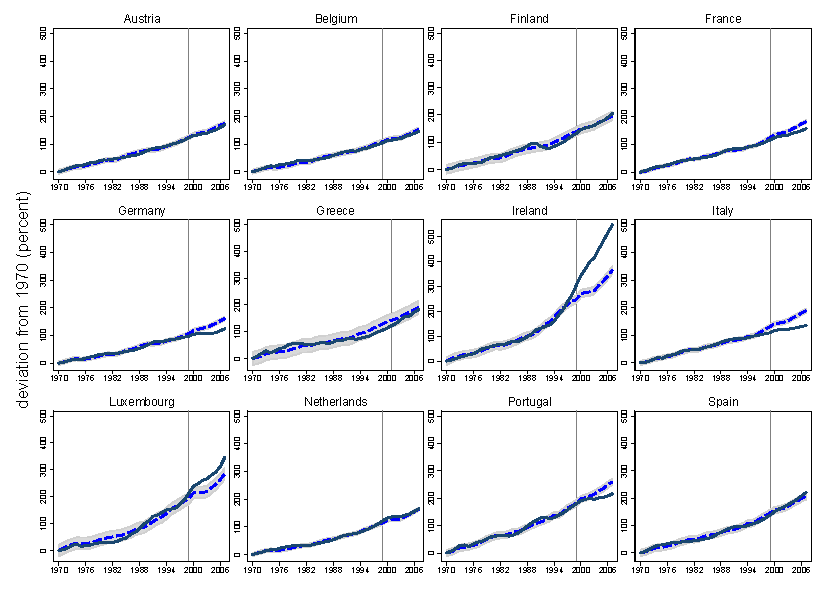
\includegraphics[scale=1.15]{SCM_gdp_Annual.pdf}
    \annote{In each graph, the dashed line represents the normalized real GDP for the synthetic country and the continuous line represents the series for the actual country. The shaded area corresponds to two standard deviations of the difference between the treated country and the doppelganger prior to the euro accession. The vertical line represents the treatment period - 1999 for all countries except for Greece which is 2001. For each country, the analysis starts in 1970 and ends in 2007.
    }
    \label{F_1}
\end{figure}

Figure \ref{F_1} displays the real GDP for each country (full black line) and doppelganger (dashed blue line) presented as the deviation from the first year of the sample in percent. The shaded area represents two standard deviations of the pre-treatment difference between the actual and the counterfactual series. When the doppelganger series deviates from the realized path in such a way that exceeds these bounds, it indicates that such deviation is non-standard compared to the pre-euro period.

A number of observations stand out. The pre-treatment paths for most countries and their doppelgangers are overlapping. Moreover, Figure \ref{F_1} shows some series embarking on a different growth trajectory relative to their counterfactuals only around the Eurozone creation. 

Table \ref{TA_Gap} presents the exact doppelganger gaps measured in euro per capita. Ireland benefited the most from the euro adoption. Its GDP per capita was 10,781 euro higher due to the common currency adoption. However, France, Germany, Italy, and Portugal would be better off by not participating in this currency union. Yet, Germany and Italy lost the most: \texteuro5,788 and \texteuro6,089 per capita respectively.

\begin{table}[h!]
\scriptsize
\caption{\label{TA_Gap} Doppelganger Output Gap}\centering
\begin{tabular}{lcccccccccccc} 
\toprule
 & \textbf{AUT}  & \textbf{BEL}  & \textbf{FIN}  & \textbf{FRA}  & \textbf{DEU}  & \textbf{GRC}  & \textbf{IRL}  & \textbf{ITA}  & \textbf{LUX}  & \textbf{NLD}  & \textbf{PRT}  & \textbf{ESP} \\
 \midrule  
\textbf{Gap} & \multirow{2}{*}{-682} & \multirow{2}{*}{-679} & \multirow{2}{*}{1,269} & \multirow{2}{*}{-2,843} & \multirow{2}{*}{-4,864} & \multirow{2}{*}{-153} & \multirow{2}{*}{10,961} & \multirow{2}{*}{-7,351} & \multirow{2}{*}{5,157} & \multirow{2}{*}{168} & \multirow{2}{*}{-3,706} & \multirow{2}{*}{1,539} \\
(\texteuro \ per capita) &  &  &  &  &  & &  & &  & &  &  \\
\bottomrule
\end{tabular}
\annote{This table presents the doppelganger output gap per capita in 2007. This measure is obtained by adjusting the real GDP gap for the population size and converting 2011 US dollars into 2011 euro. We use the conversion rate available from the PWT 9.1 for this year ($\approx 0.73$).}
\end{table}

\subsection{Causality \label{SS_Causality}}

A key assumption to study the impact of a policy intervention is that there is no reverse causality. In our context, this means that countries must not have adopted the euro due to economic considerations. This assumption is plausible because the Eurozone accession was driven mainly by political rather than economic factors \citep{Feldstein1997, Dyson1999, Willett2000, Spolaore2013}.\footnote{This argument holds even for the Greek case which had decided to join the euro before the single currency was a reality. According to the 1998 convergence report from the European Commission, Greece did not join the single currency in 1999 because it had not fulfilled any of the four convergence criteria. Notwithstanding, the decision to join was already made.} The adoption of the Euro was seen more as a political project aimed at deepening European integration; reducing the risks of conflict; and creating a stronger Europe on the global affair \citep{Eichengreen1993, James2012}. 

\cite{Feldstein1997} found that the economic impact of joining the EMU would be uncertain, with the possibility of some small gains in trade and investment, accompanied by larger unemployment and inflation. \cite{Fernandez2013} studies the mechanisms through which the adoption of the Euro delayed, rather than advanced, economic reforms in some Eurozone countries.

Moreover, the Euro area is not considered an optimal currency area (OCA), which casts doubt on the strength of the economic motivations behind its adoption. According to \citep{Mundell1961}, OCA have labor mobility, capital mobility, a risk-sharing system such as a fiscal transfer mechanism, and similar business cycles among the member countries. Labor mobility was limited by language and cultural barriers, and there was significant divergence in economic conditions and fiscal policies among the member states. Importantly, by not satisfying the requirements of an Optimum Currency Area, many economists believed that some countries adopting the euro would face economic losses \citep{Jonung2009}.

Even though there are expected gains in terms of real economic growth from adopting a fixed exchange regime, that is not expected for all countries alike; \cite{Arvai2023} provide evidence that countries with less credible monetary policy are the ones growing after pegging their currency to a more credible anchor.  

Sections \ref{SS_Implementation} and \ref{SS_Data} discussed the conditions under which the SCM provides suitable estimates of causal effects and this section addresses some of these requirements. To further back the notion that the doppelganger gap is indeed caused by the euro adoption, Sections \ref{SS_timeplacebo} and \ref{SS_spaceplacebo} provide two key placebo experiments. We can be confident that the synthetic control estimator captures the causal effect of an intervention as long as similar magnitudes are not estimated in cases where the intervention did not take place \citep{Born2018}. Finally, Section \ref{SS_stat} discusses the statistical significance of the results. 

%Argue that treatment is ``as good as random" and that there are no sources of reverse causality in our analysis. That is, countries must not have adopted the euro to stimulate economic growth. This assumption is plausible because the Eurozone accession was driven mainly by political rather than economic factors \citep{Eichengreen1993} and \cite{Feldstein1997}). This argument holds even for the Greek case which had decided to join the euro before the single currency was a reality.\footnote{According to the 1998 convergence report from the European Commission, Greece did not join the single currency in 1999 because it had not fulfil any of the four convergence criteria. Notwithstanding, the decision of joining was already made.}
%(From \cite{Puzzello2018}) A key assumption on which the identification of the synthetic estimator rests is that endogeneity is not due to reverse causation. In the context of our application, this is equivalent to ruling out the possibility that countries adopted the euro because they expected it would spur their future economic growth. If synthetic estimates of the intervention effect were affected by endogeneity, our estimated gaps in the cases when the treated unit does better than the synthetic unit would be upward biased, while all the remaining estimated gaps would be downward biased. Having said that, we are not overly concerned that endogeneity is an issue as the literature suggests that euro adopters gave up their national currencies mainly for political reasons. In fact, economic accounts of the costs and benefits of adopting the euro in the 1990s agree that the EMU was not an OCA, it would lead to economic losses for all countries involved and was to be understood mainly as a political phenomenon (Eichengreen and Frieden, 1993; Feldstein, 1997). In other words, even though economic considerations were part of the political discussions at the national level, they were not the main reasons behind the decision to adopt the euro for early adopters.



\subsubsection{In-Time Placebo Test: Anticipation Effects \label{SS_timeplacebo}}

On 7 February 1992, representatives from twelve countries signed the Maastricht Treaty  – Belgium, Denmark, France, Germany, Greece, Ireland, Italy, Luxembourg, Netherlands, Portugal, Spain, and the United Kingdom. Upon signing it, it was common knowledge that a monetary union, with a central banking system and a common currency, was to be created within the next years. It is, therefore, reasonable to think that countries experienced, at least partly, the Eurozone accession's impact before the euro was launched. 

To check for anticipation effects of the euro adoption, we perform in-time placebo tests by inspecting different intervention periods in our analysis. The date the Maastricht Treaty was signed is taken as the placebo treatment period. Figure \ref{F_Maastricht} suggests that the main conclusions from Figure \ref{F_1} remain unchanged.

We ran further time-placebo tests in which the placebo treatment date is set artificially to be every year from 1992 until 1998. For the sake of brevity, besides the Maastricht Treaty date 1992, we only report the tests for 1995 and 1998 in Figures \ref{F_1995} and \ref{F_1998}. Reassuringly, the results remain unaltered.\footnote{The remaining figures can be provided by the authors upon request.}

\begin{figure}[h!]
    \centering
    \caption{In-time Placebo Tests}
    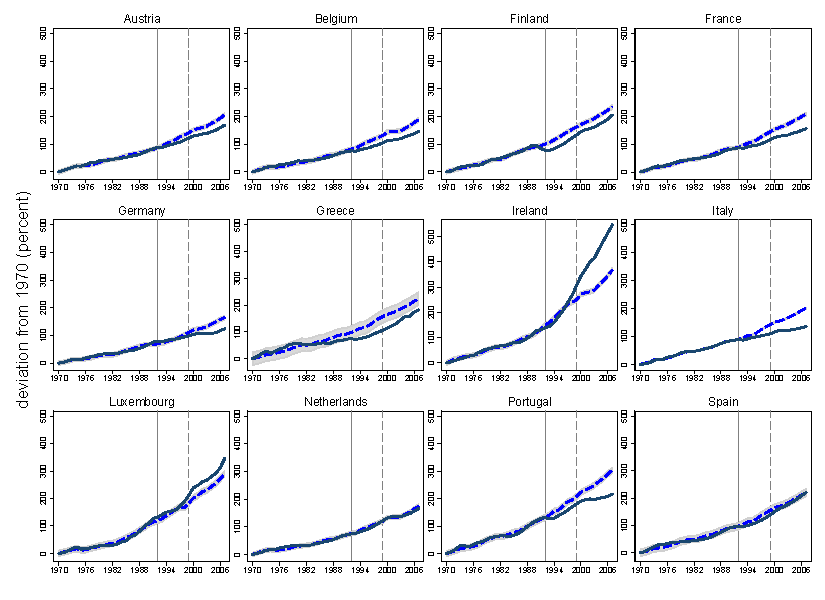
\includegraphics[scale=1.2]{Output/Figures/SCM_gdp_Rob_1992_Annual.pdf}
    \annote{In each graph, the blue dashed line represents the normalized real GDP for the synthetic country and the black full line represents the series for the actual country. The shaded area corresponds to two standard deviations of the difference between the treated country and the doppelganger prior to the euro accession. The vertical line depicts the placebo treatment period - 1992 for all countries. For all countries, the analysis starts in 1970 and ends in 2007. %The baseline specification has as predictors labor productivity growth, employment share, and GDP shares from PENN Tables 9.1 data. OECD restricted donor pool.
    }
    \label{F_Maastricht}
\end{figure}

Figure \ref{F_Maastricht} presents limited evidence in favor of the existence of anticipation effects. If anything, the gap between the actual and the synthetic series becomes wider than the one analyzed in Figure \ref{F_1}. Notwithstanding, the direction of the effect remains unchanged. Thus, ignoring possible anticipation effects in our baseline estimates may lead to a lower bound of the euro impact for countries like Austria, Belgium, France, and Italy.\footnote{The case for Greece is not worrisome given its bad pre-treatment fit and, therefore, its lack of significance.}

The absence of anticipation effects for the remaining countries may be due to two things. First, the key event representing a change for most European citizens was the irrevocable exchange rate fix on 31st December 1998 and the euro launch on the 1st of January 1999. Second, most of these countries had already experienced trade and economic gains from joining the European Union \citep{Campos2018}. Therefore, such effects lie in our pre-treatment sample and thus, are already being considered.\footnote{Add the fact that Italy dropped the exchange rate agreement and floated for a year 93-94. Add that Austria and Finland joined the EU in 1995. Add that most of the divide might come from austerity measures implemented in Austria, Belgium, Finland, France, Germany, Italy \citep{Alesina2019}. Gabriel et al. 2023 ReStat, show how recessionary were these spending based austerity shocks implemented, also following the Maastricht Treaty.}
%Still, these figures should be analysed carefully. For example, the plot for Greece shows some effect that starts even before the placebo treatment of 1992. This anticipated effect seems to be driven by the Greek European Union (EU) accession in 1981 and not from the Euro. 
%Furthermore, estimates for Austria and Finland must be interpreted carefully as these countries entered the EU exactly in 1995 and the placebo treatment effect may be biased. 


\subsubsection{In-Space Placebo Test \label{SS_spaceplacebo}}

Following \cite{Abadie2010}, \cite{Abadie2018}, and \cite{Firpo2018}, we employ the synthetic control methodology on the donor pool countries while exposing them to a placebo treatment in 1999. The idea is to sequentially ``re-assign" the treatment to all units in the donor pool and, for each of them, estimate a fictitious doppelganger using the remaining donor countries and the originally treated unit. We repeat this process for every treated country.

Next, we compare the post and pre-treatment behavior of these series and inspect the differences between treated and fictionally treated units. If our benchmark estimates for each Eurozone country are picking up the causal effect of the euro accession, these should dominate any possible impact of the fictitious event in the donor countries. On the other hand, if no difference is found, then most likely the actual intervention had no effect. Applying this idea to each country in the donor pool allows us to compare the estimated effect of the euro accession on Eurozone countries to the distribution of placebo effects obtained for the other countries \citep{Abadie2015}.

%Intuitively, this exercise allows us to examine whether or not the estimated effect of the euro adoption is large relative to the distribution of the effects estimated for the GDP of non-adopting countries.

\begin{figure}[h!]
		\centering
		\caption{In-Space Placebo Tests}	\label{F_Placebo}
	    \subfigure[Austria]{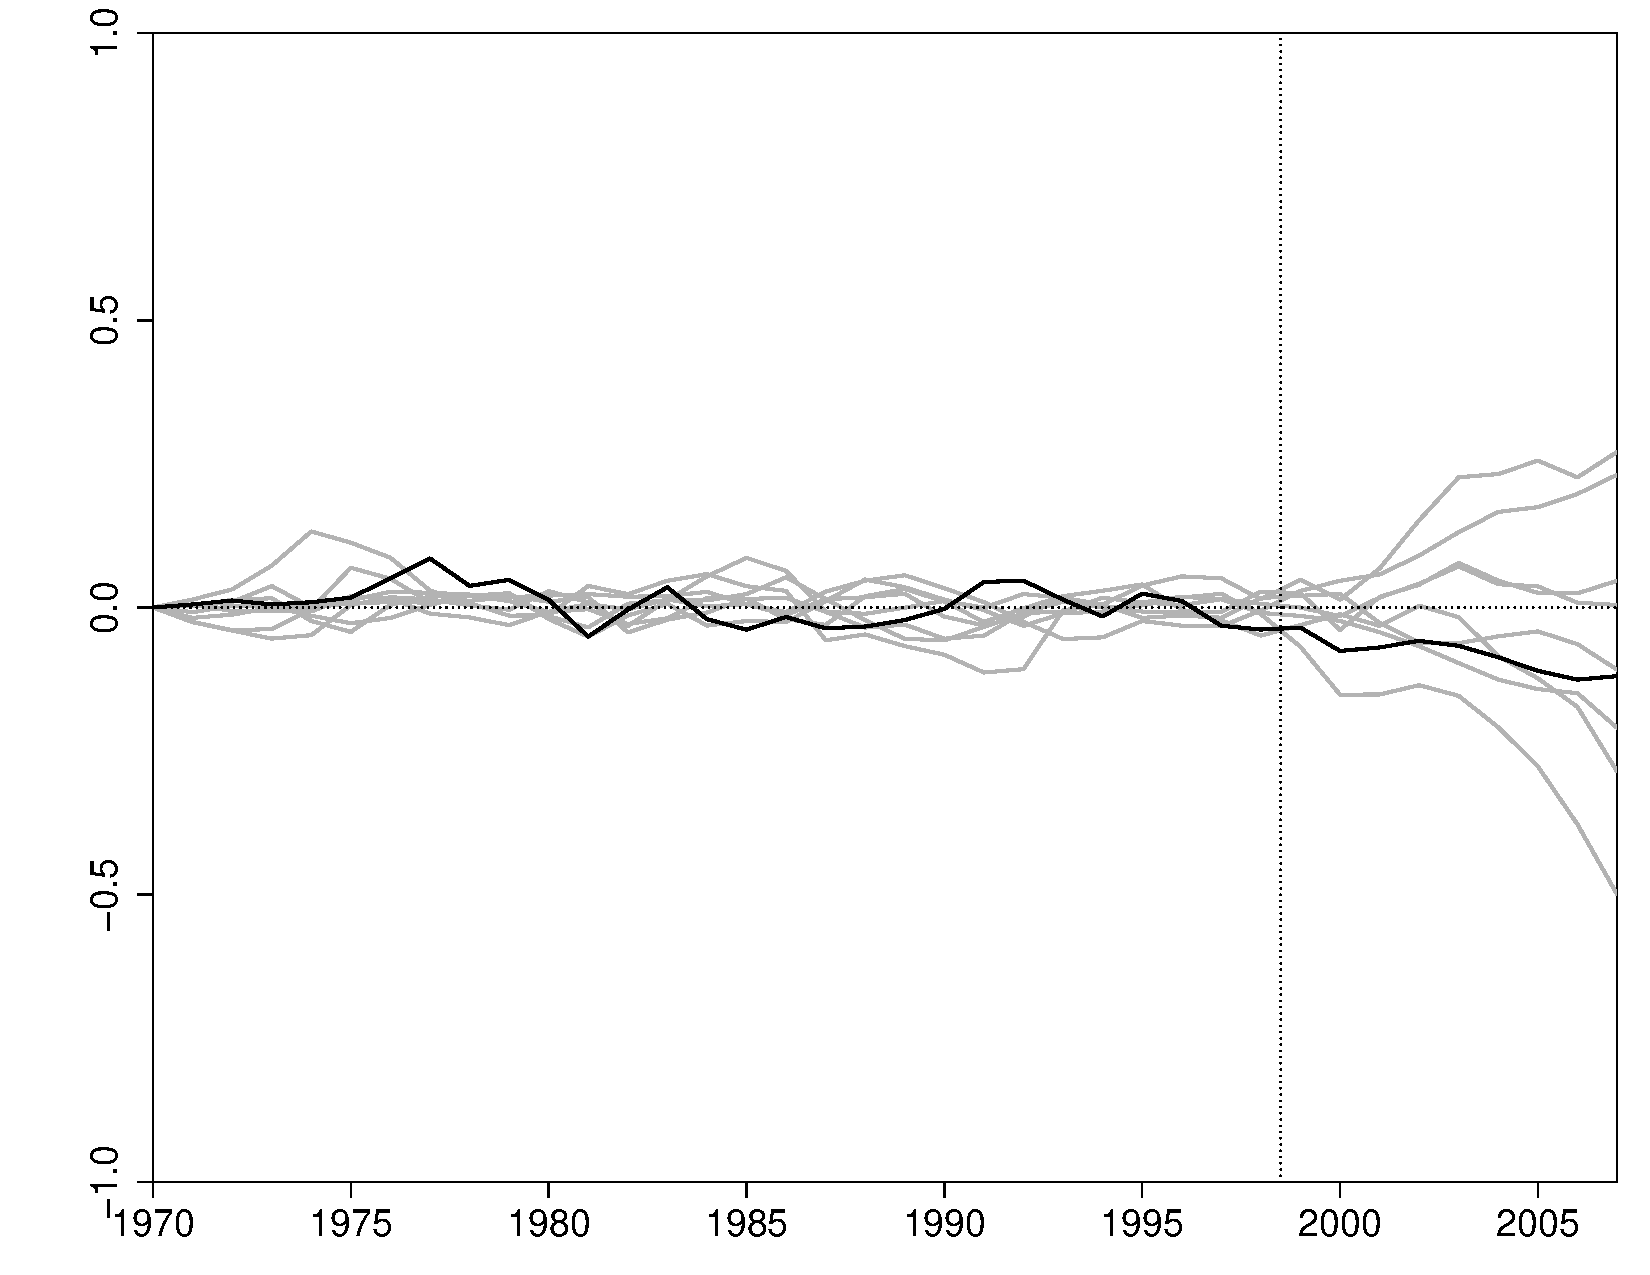
\includegraphics[width=5cm]{graph_placebo_effects_excluding_outliers_15.pdf}}
	    \subfigure[Belgium]{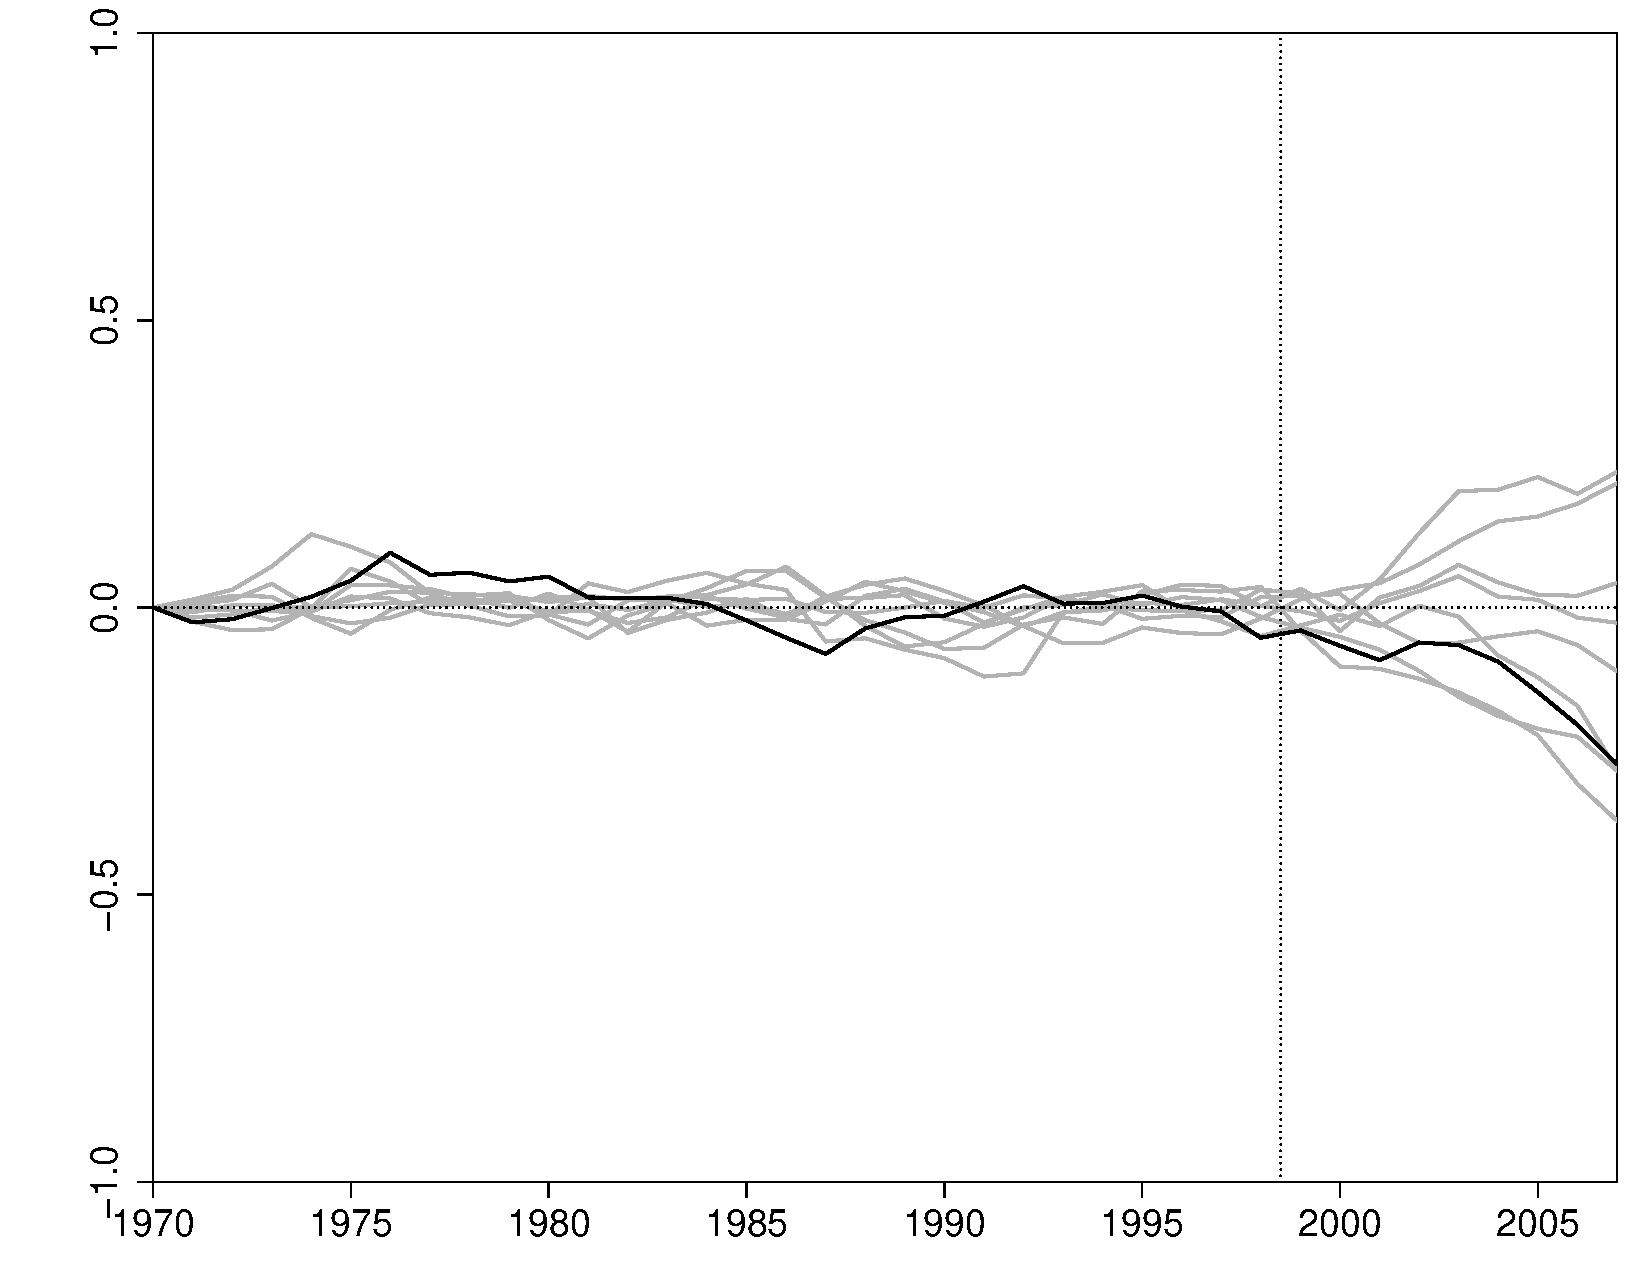
\includegraphics[width=5cm]{graph_placebo_effects_excluding_outliers_16.pdf}}
	    \subfigure[Finland]{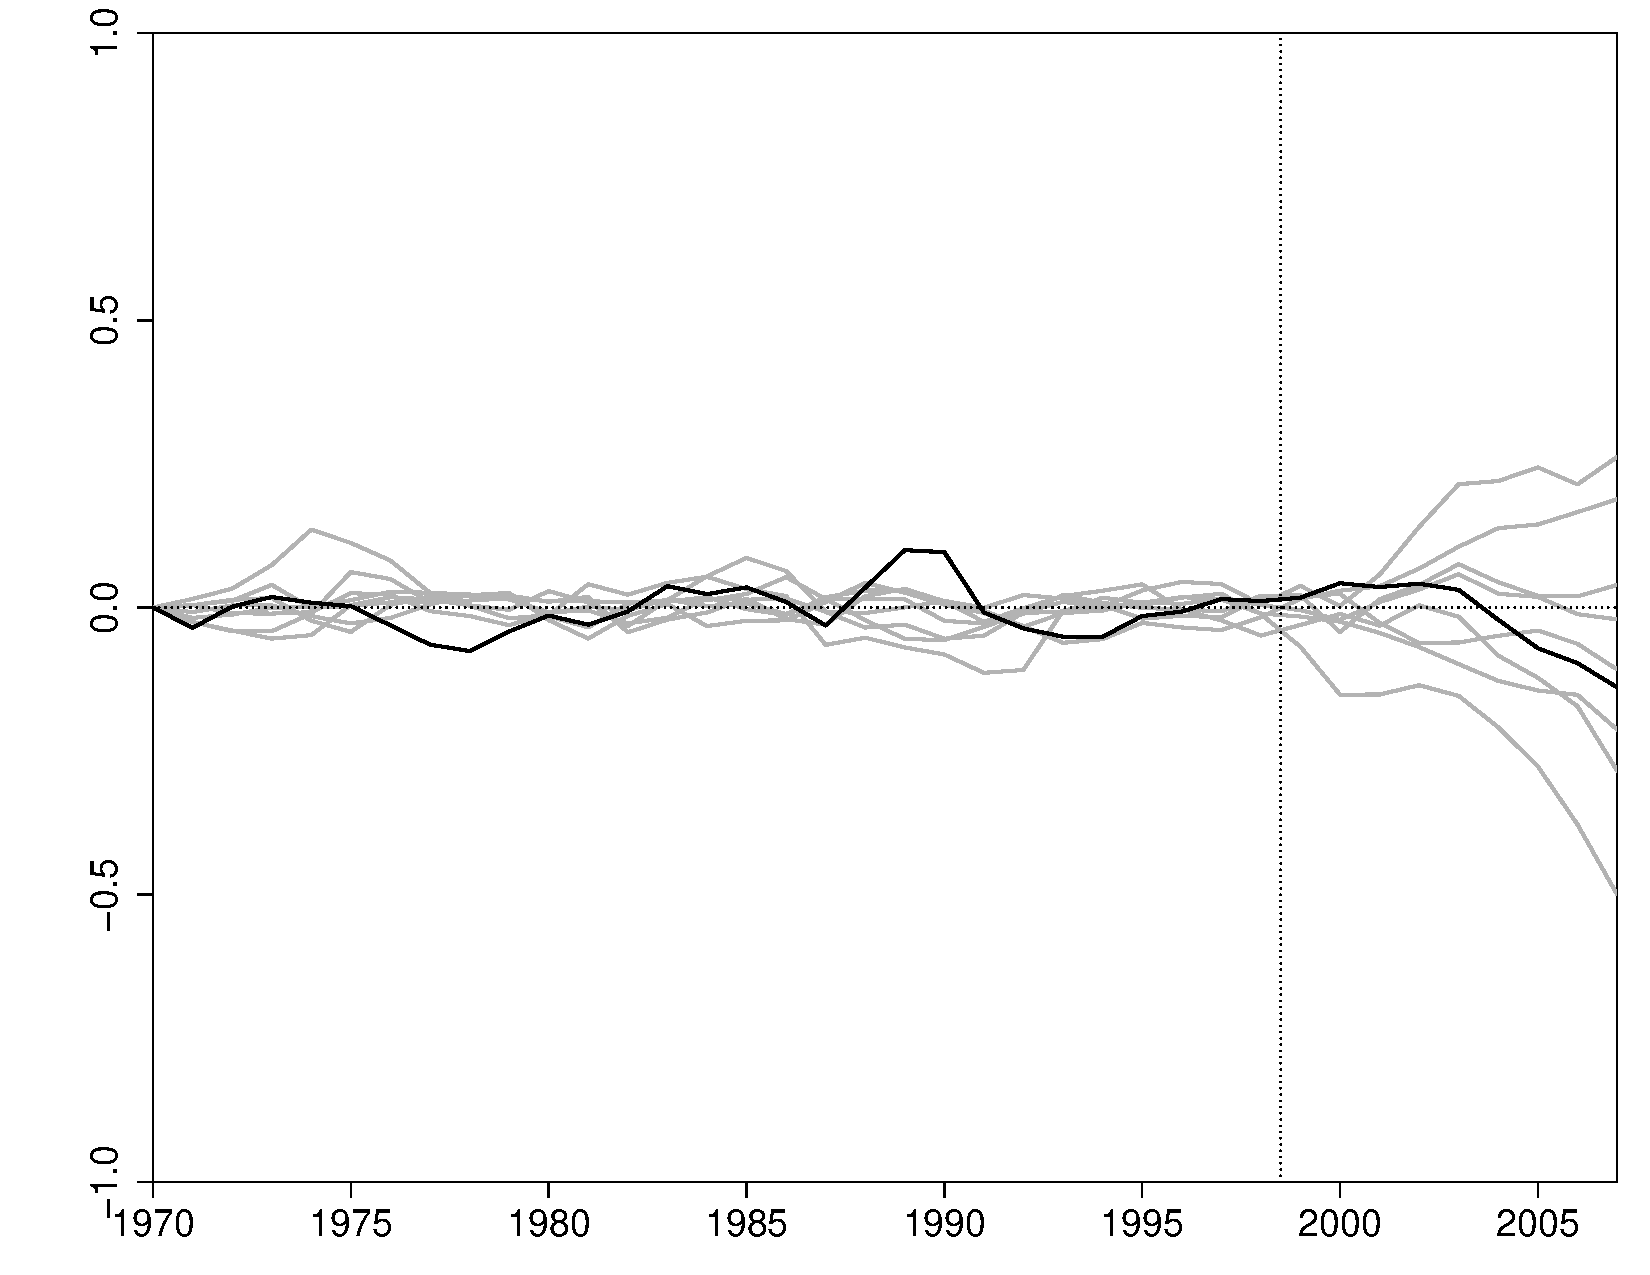
\includegraphics[width=5cm]{graph_placebo_effects_excluding_outliers_17.pdf}}		
		\subfigure[France]{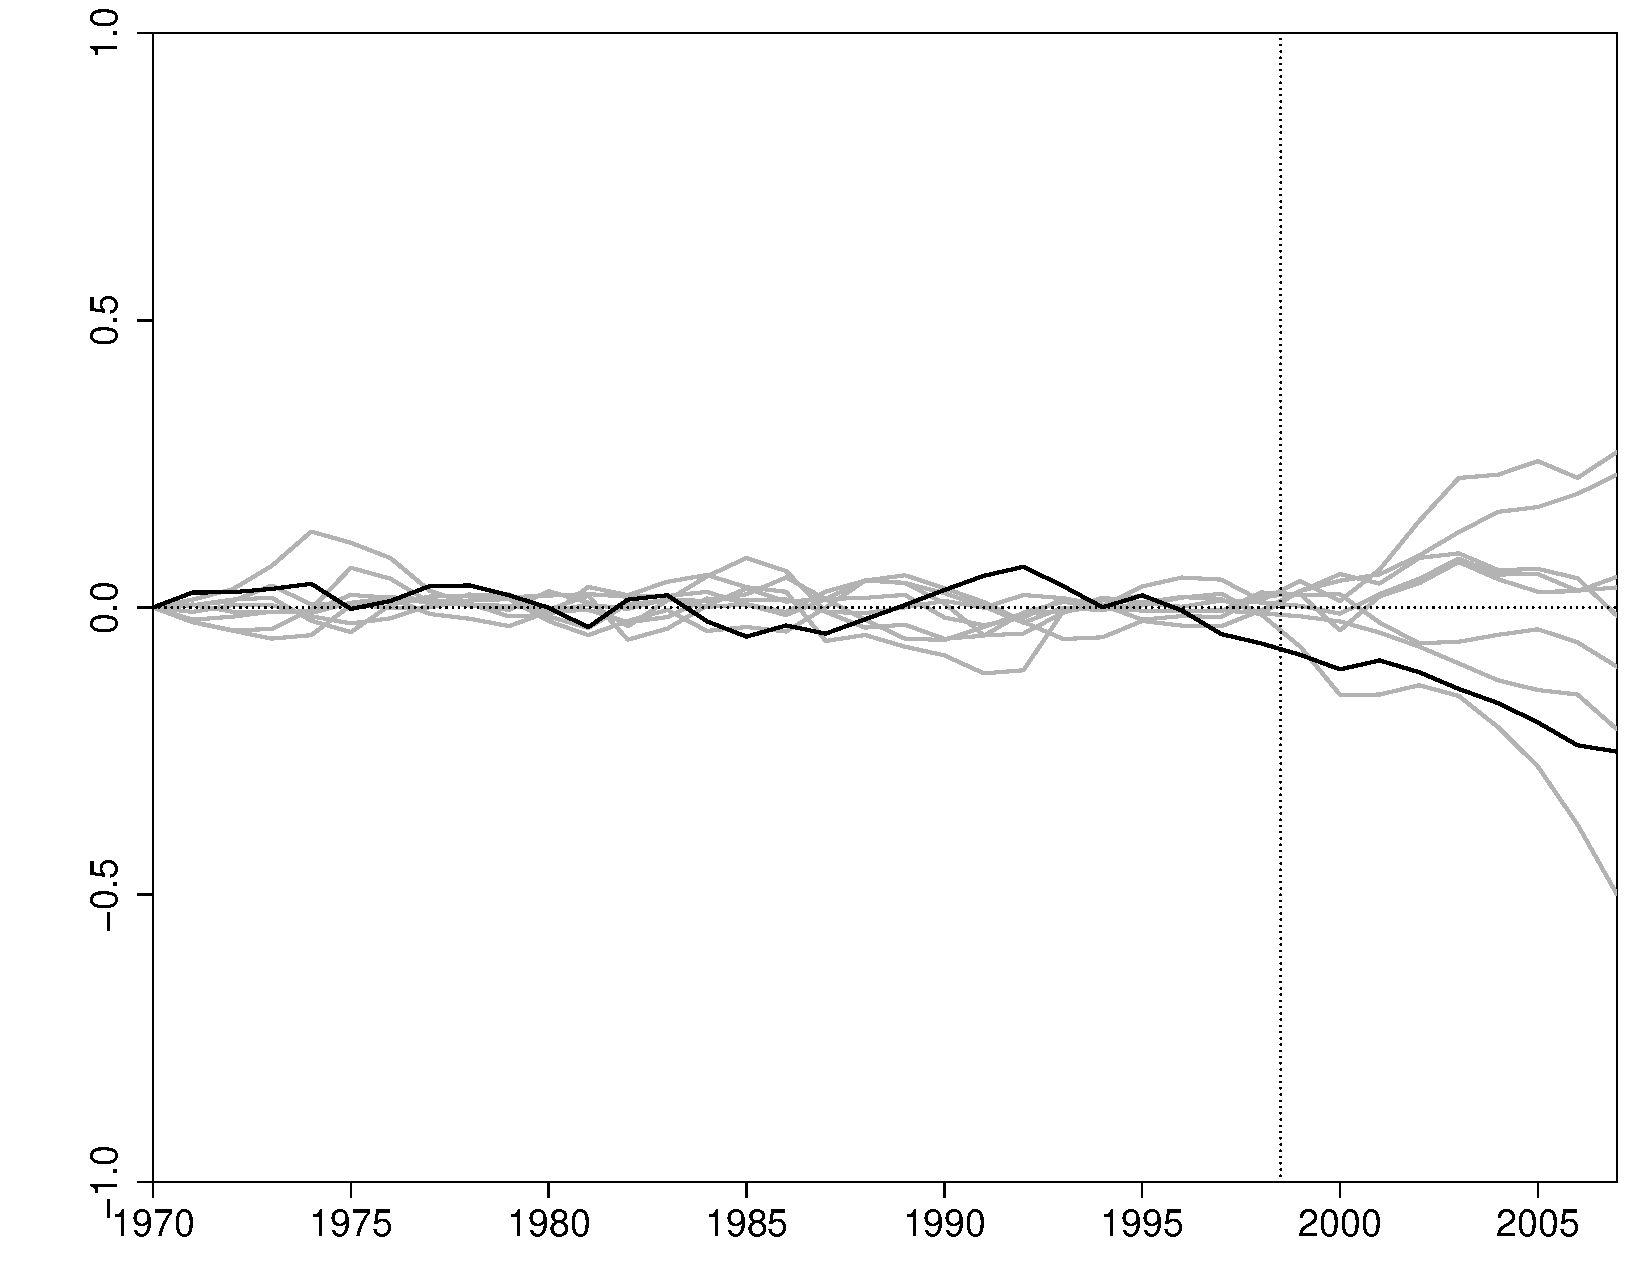
\includegraphics[width=5cm]{graph_placebo_effects_excluding_outliers_18.pdf}}
		\subfigure[Germany]{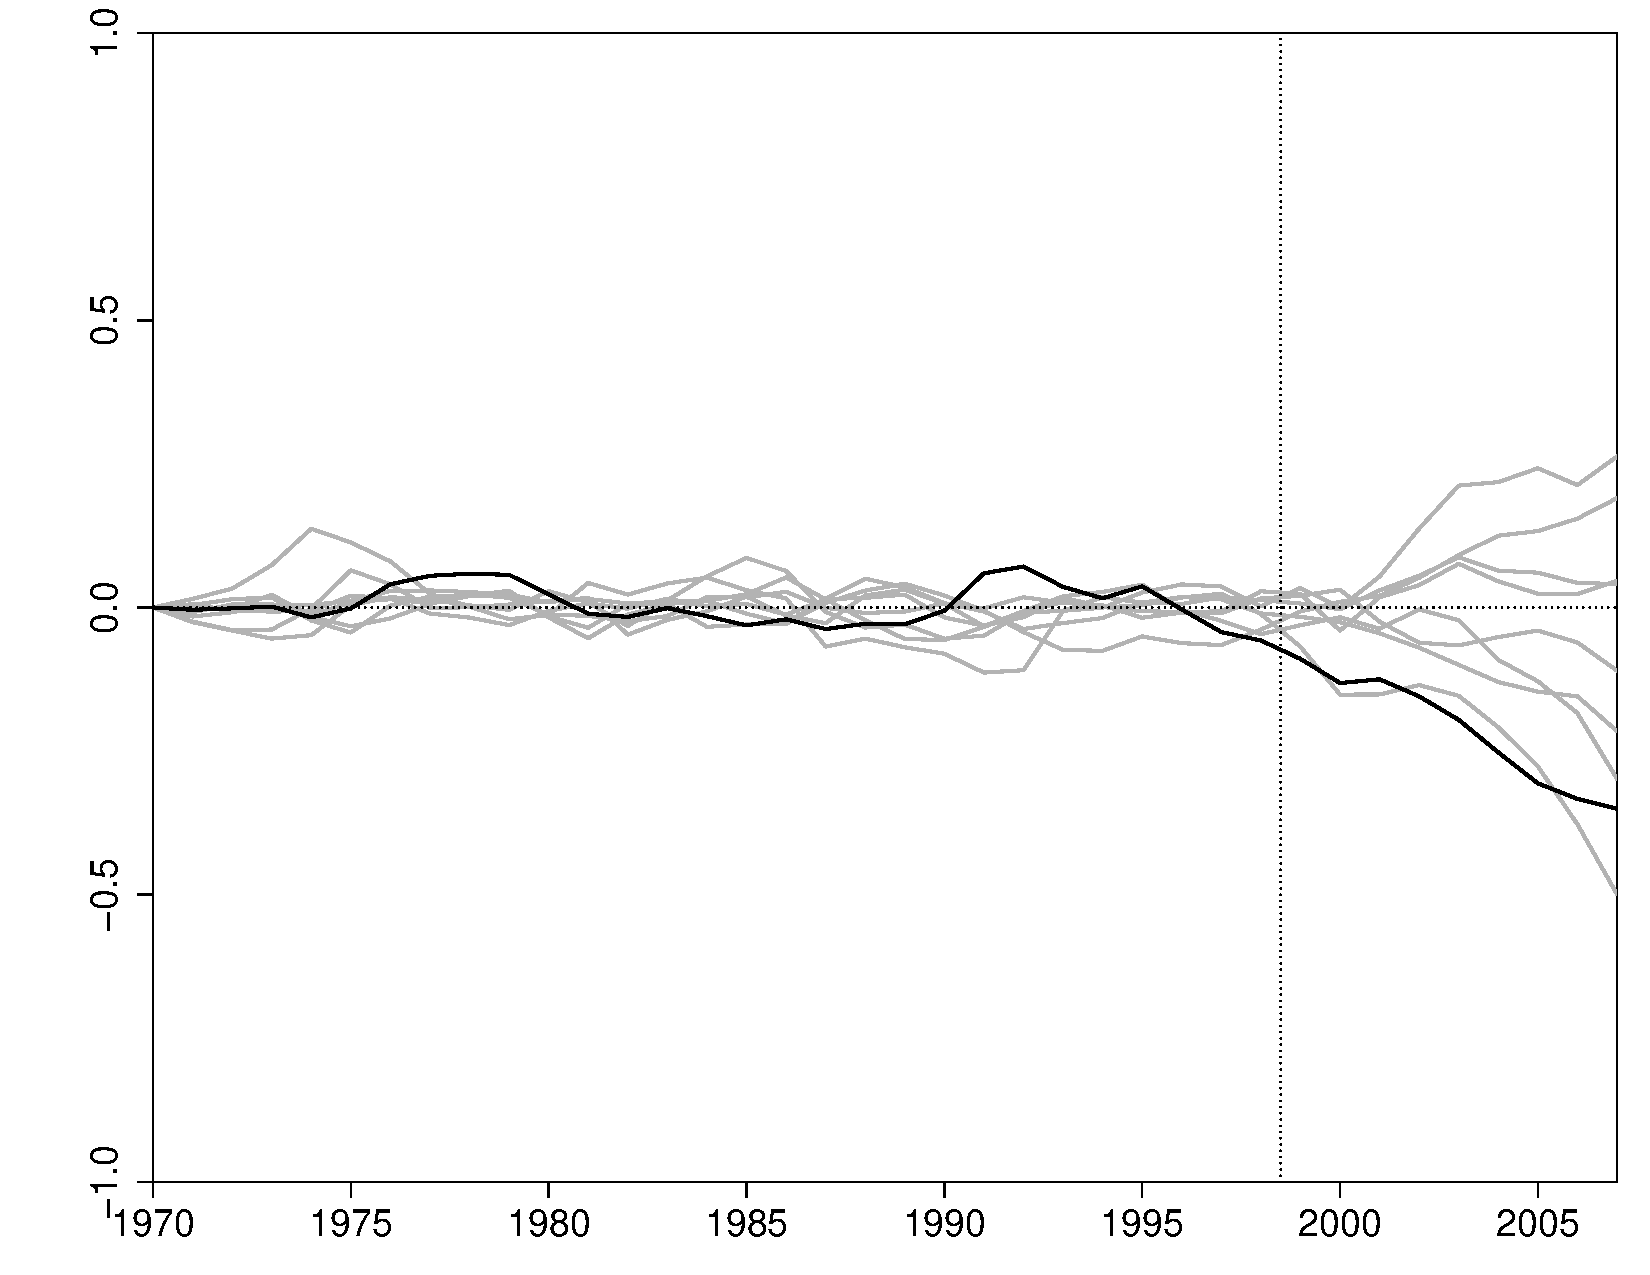
\includegraphics[width=5cm]{graph_placebo_effects_excluding_outliers_19.pdf}}
		\subfigure[Greece]{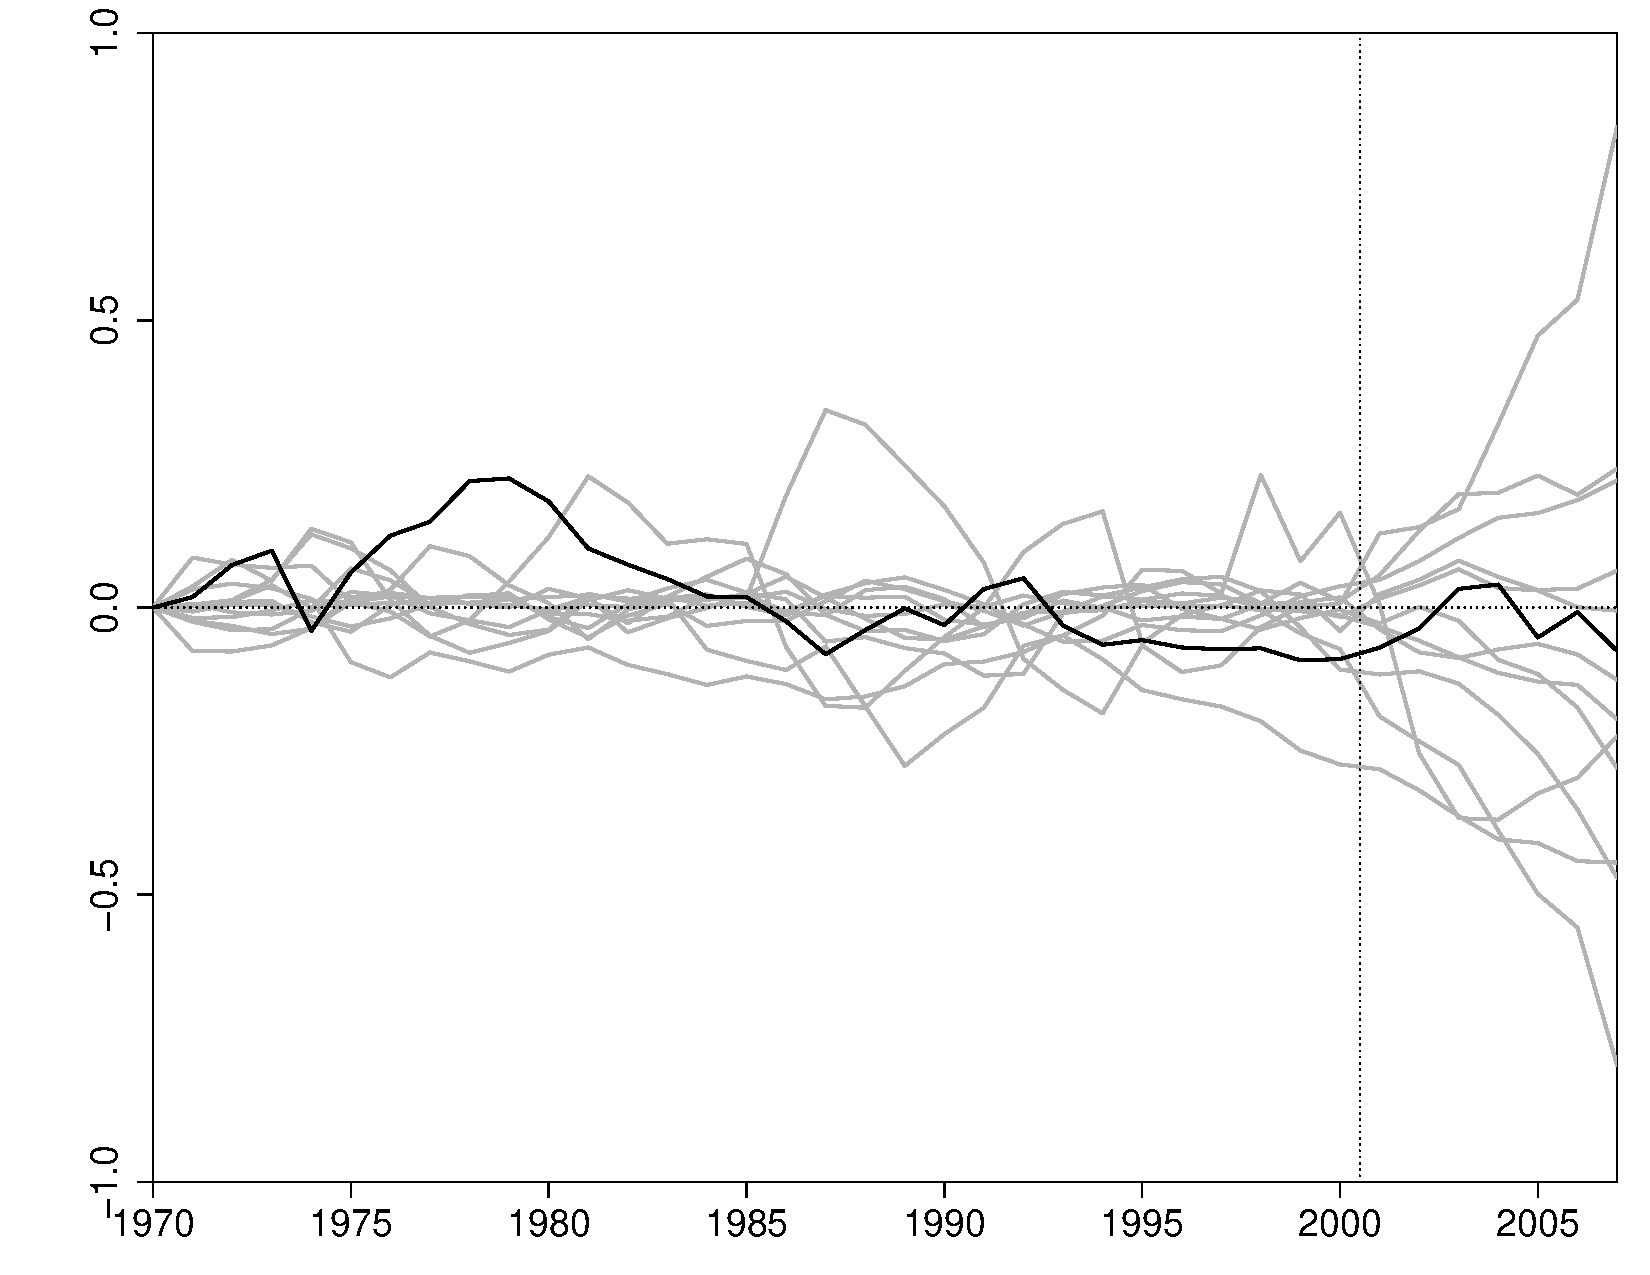
\includegraphics[width=5cm]{graph_placebo_effects_excluding_outliers_20.pdf}}
		\subfigure[Ireland]{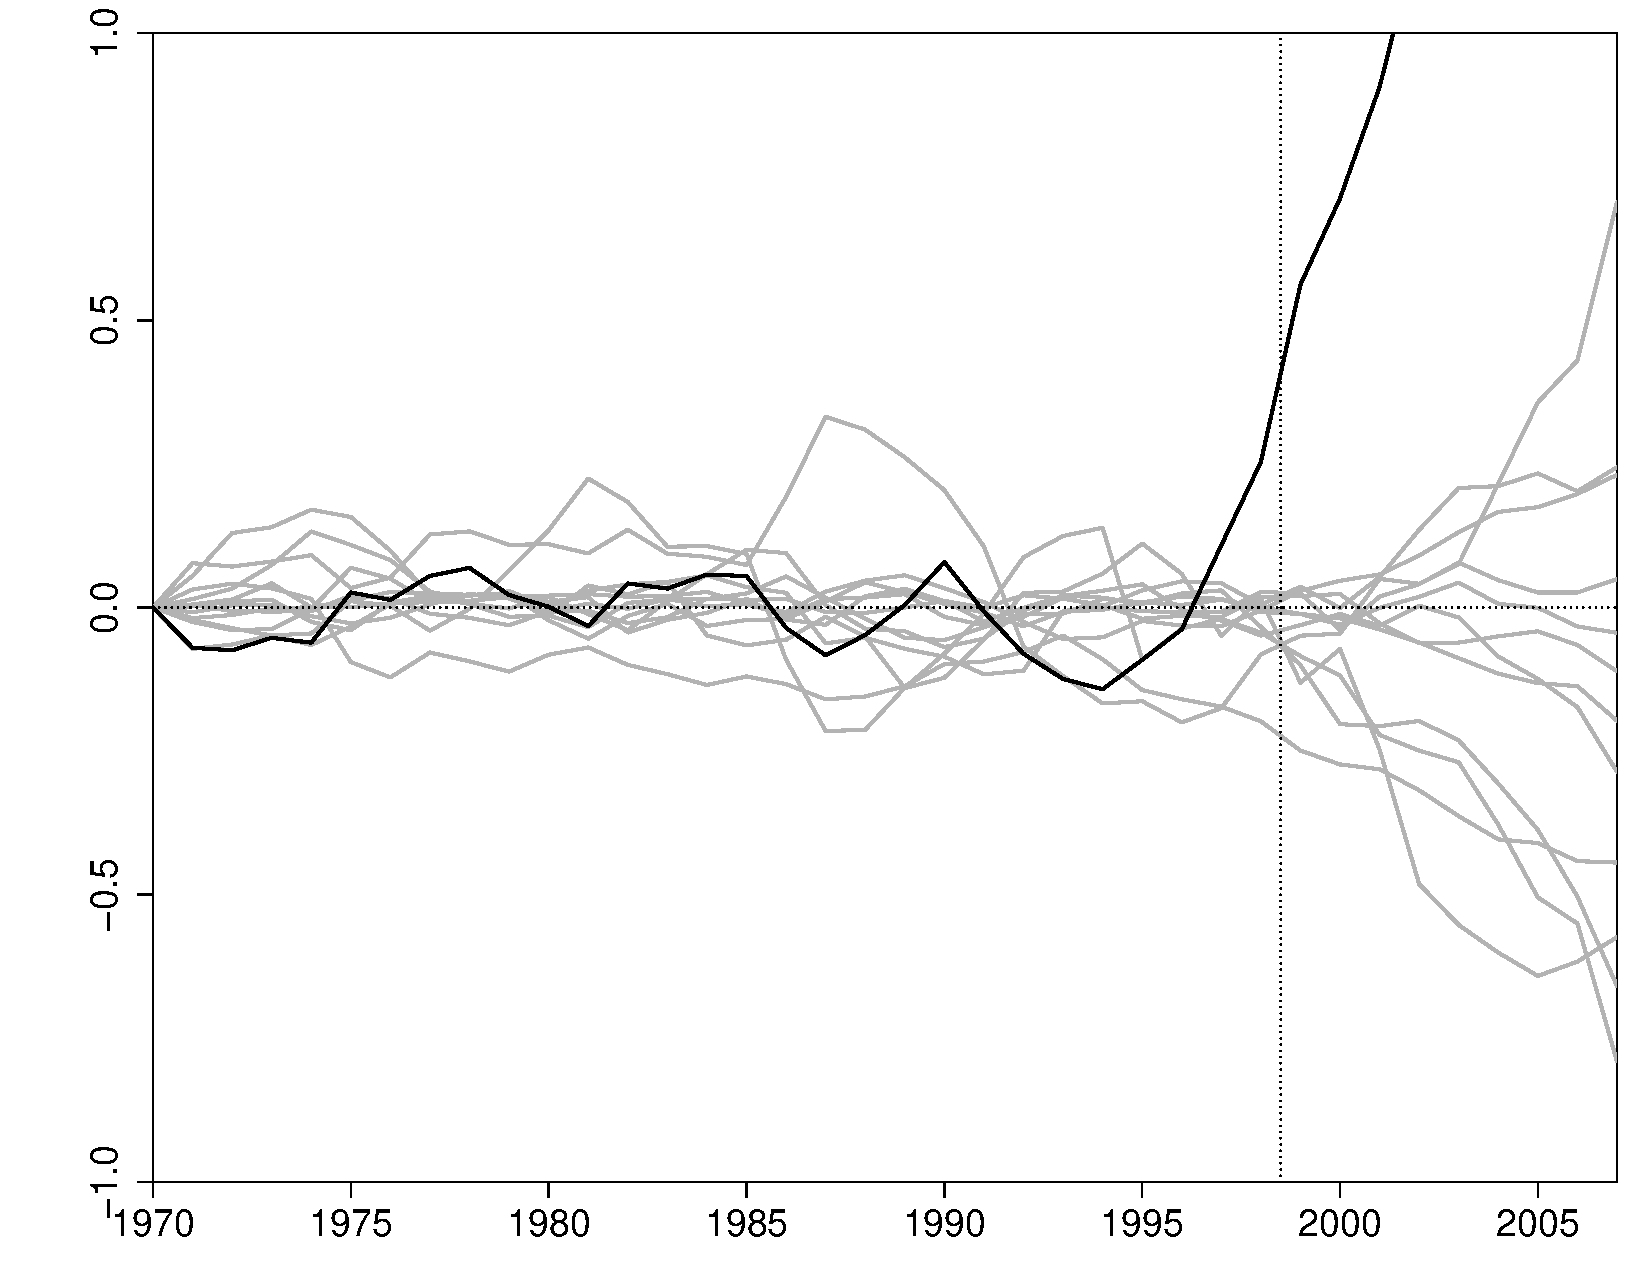
\includegraphics[width=5cm]{graph_placebo_effects_excluding_outliers_21.pdf}}
		\subfigure[Italy]{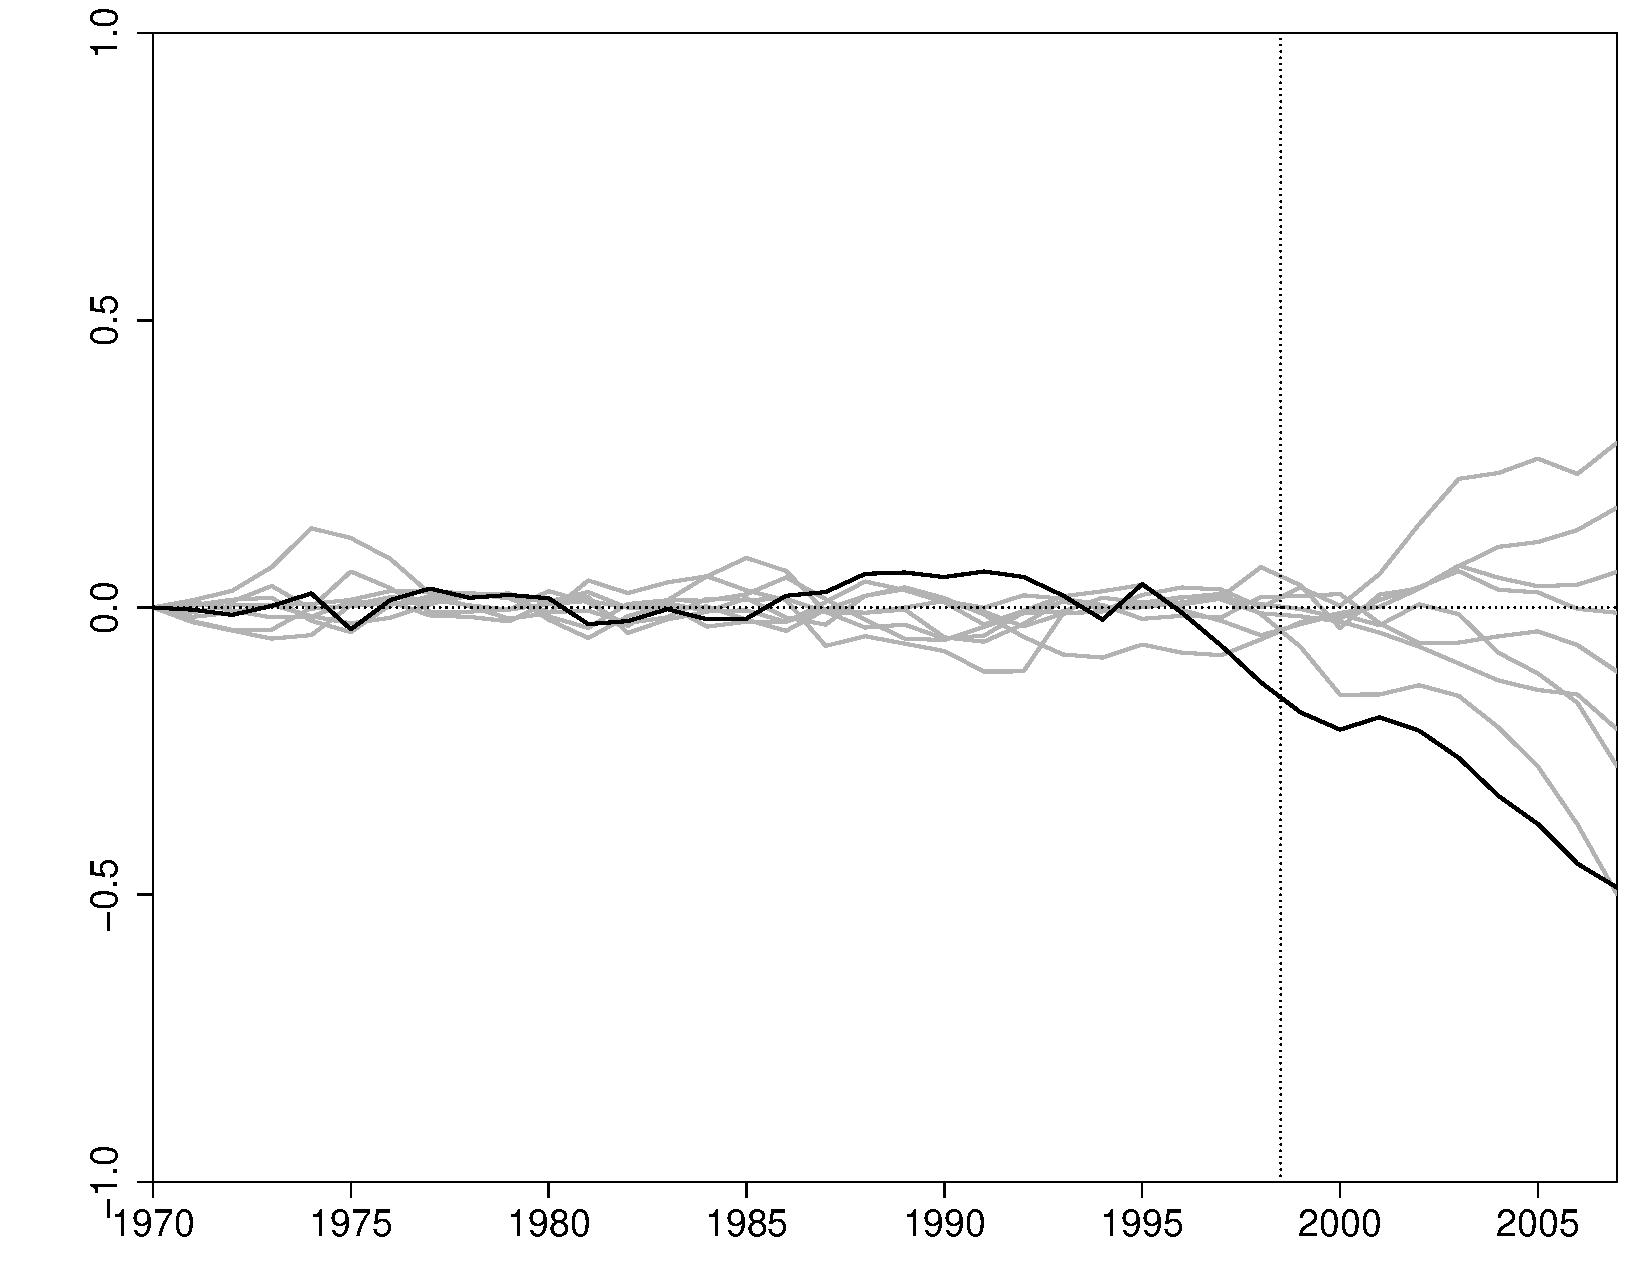
\includegraphics[width=5cm]{graph_placebo_effects_excluding_outliers_22.pdf}}
		\subfigure[Luxembourg]{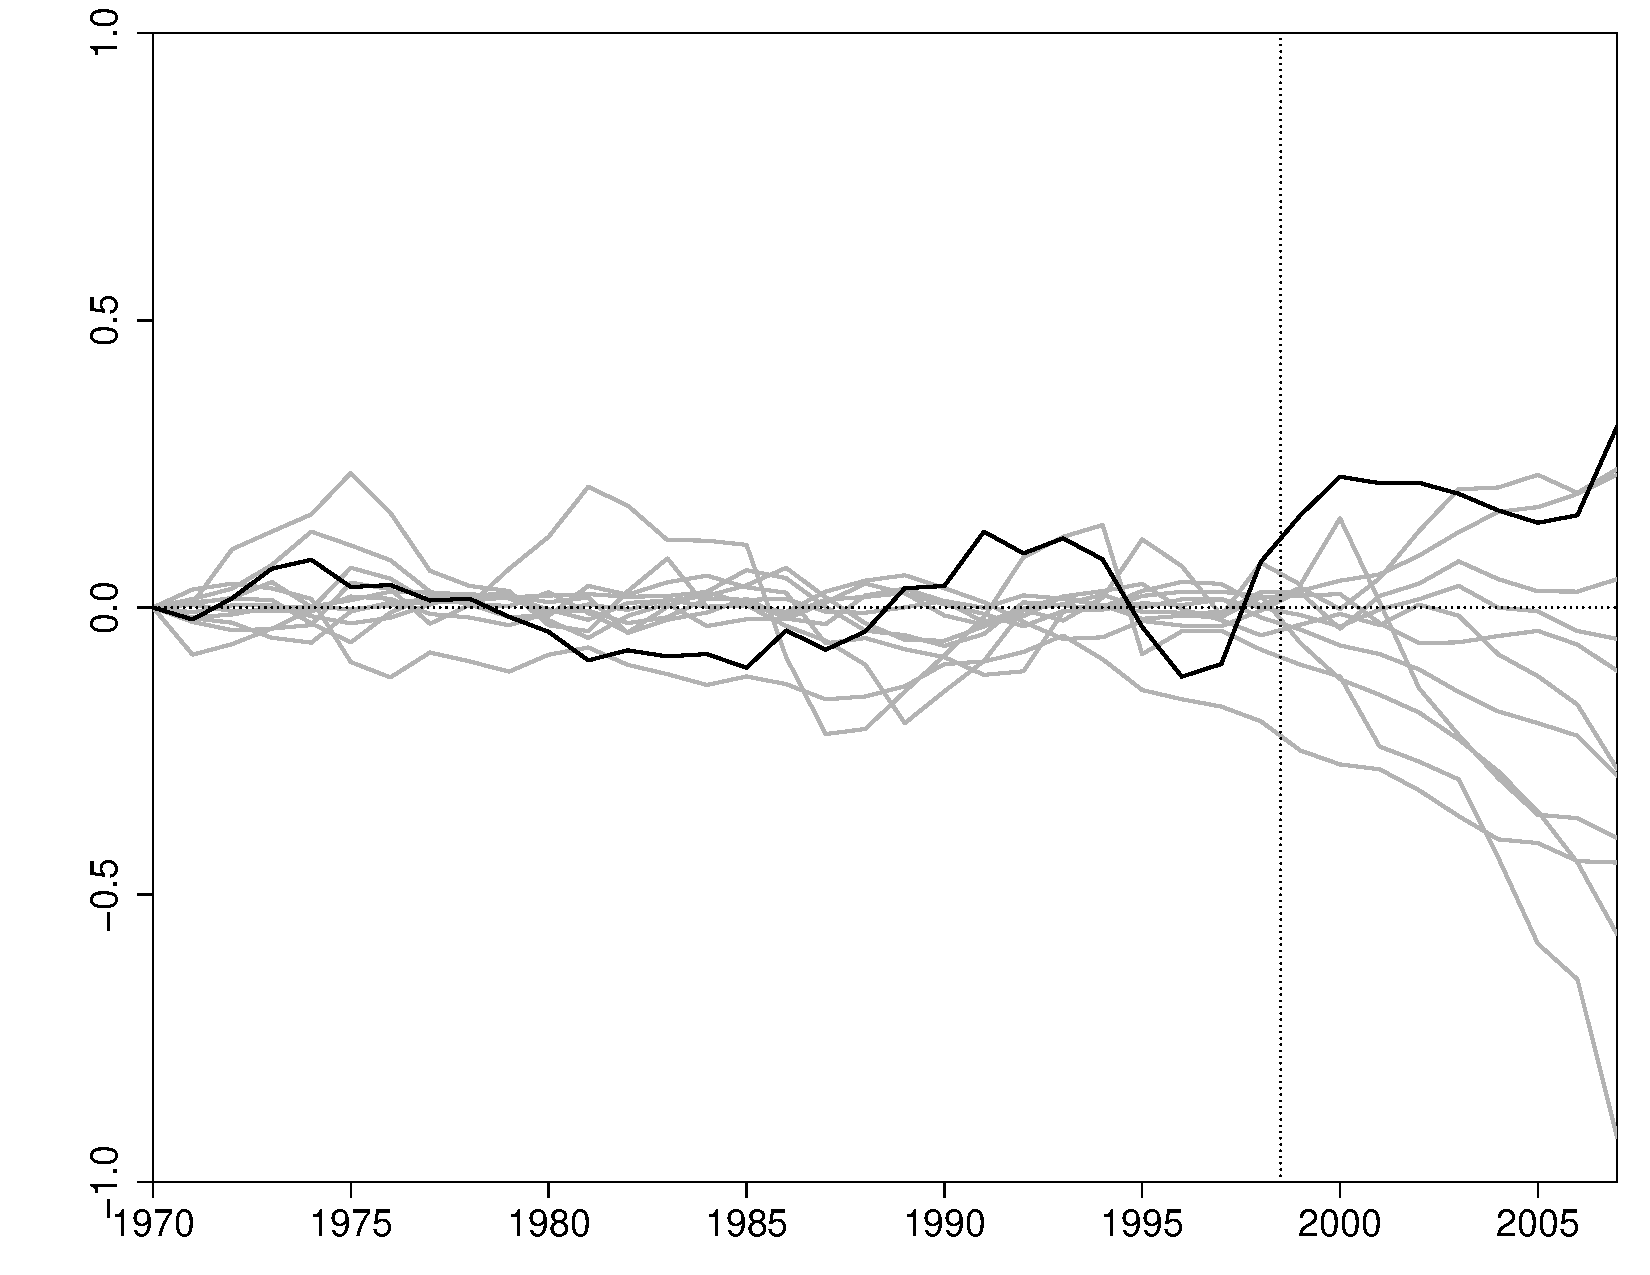
\includegraphics[width=5cm]{graph_placebo_effects_excluding_outliers_23.pdf}}
		\subfigure[The Netherlands]{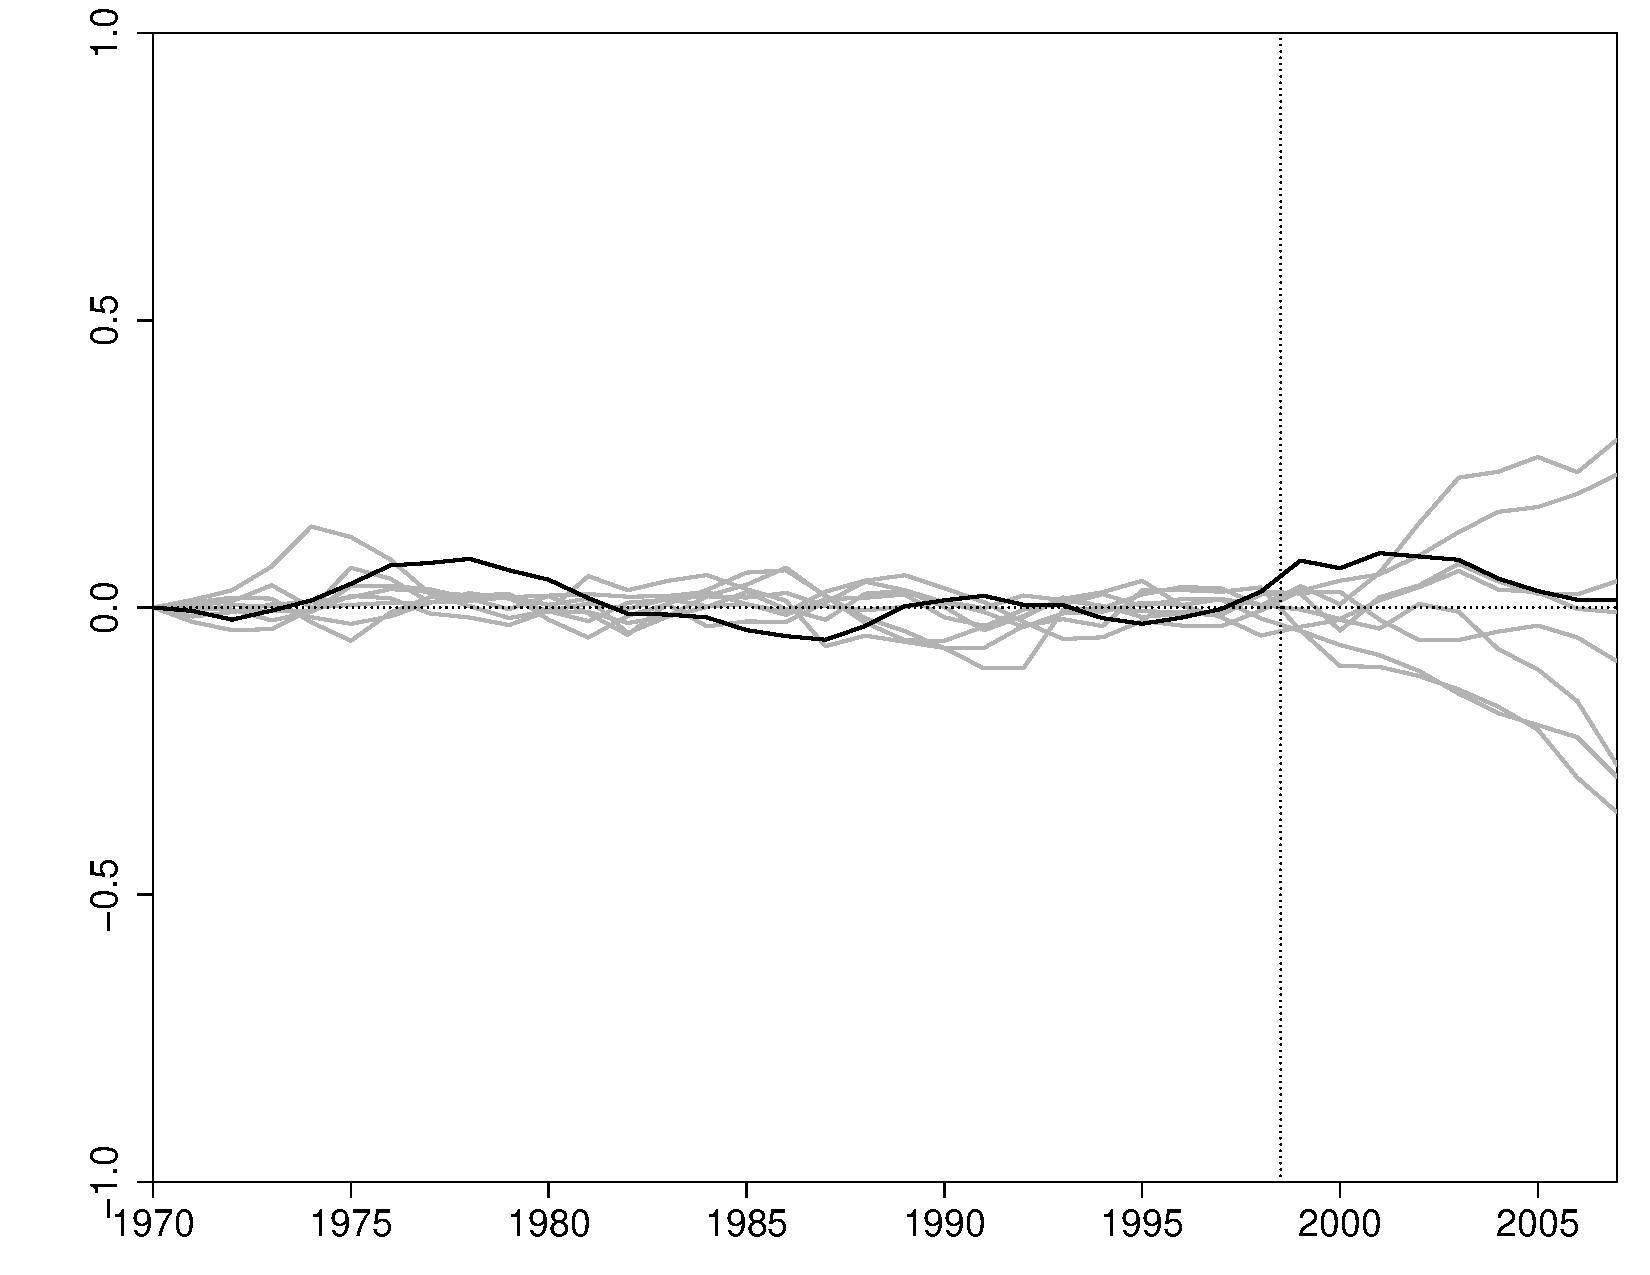
\includegraphics[width=5cm]{graph_placebo_effects_excluding_outliers_24.pdf}}
		\subfigure[Portugal]{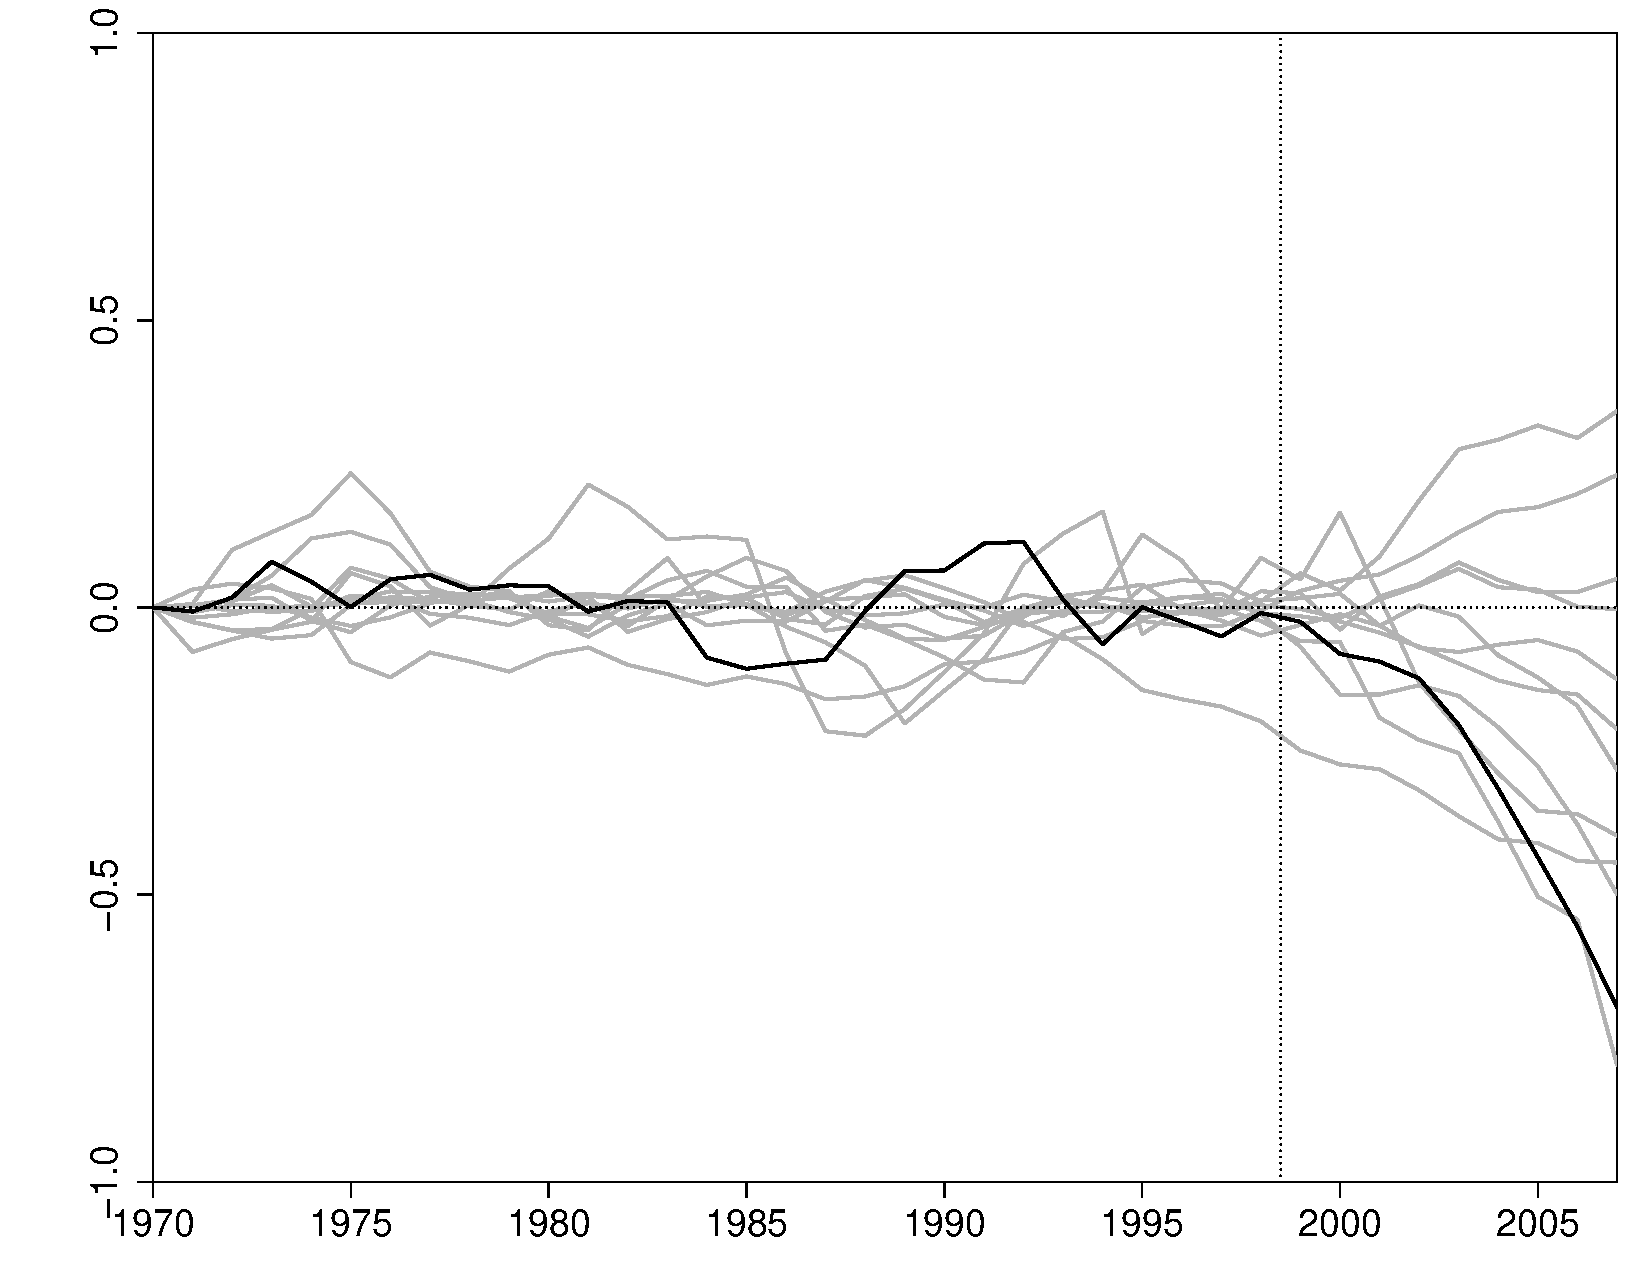
\includegraphics[width=5cm]{graph_placebo_effects_excluding_outliers_25.pdf}}
		\subfigure[Spain]{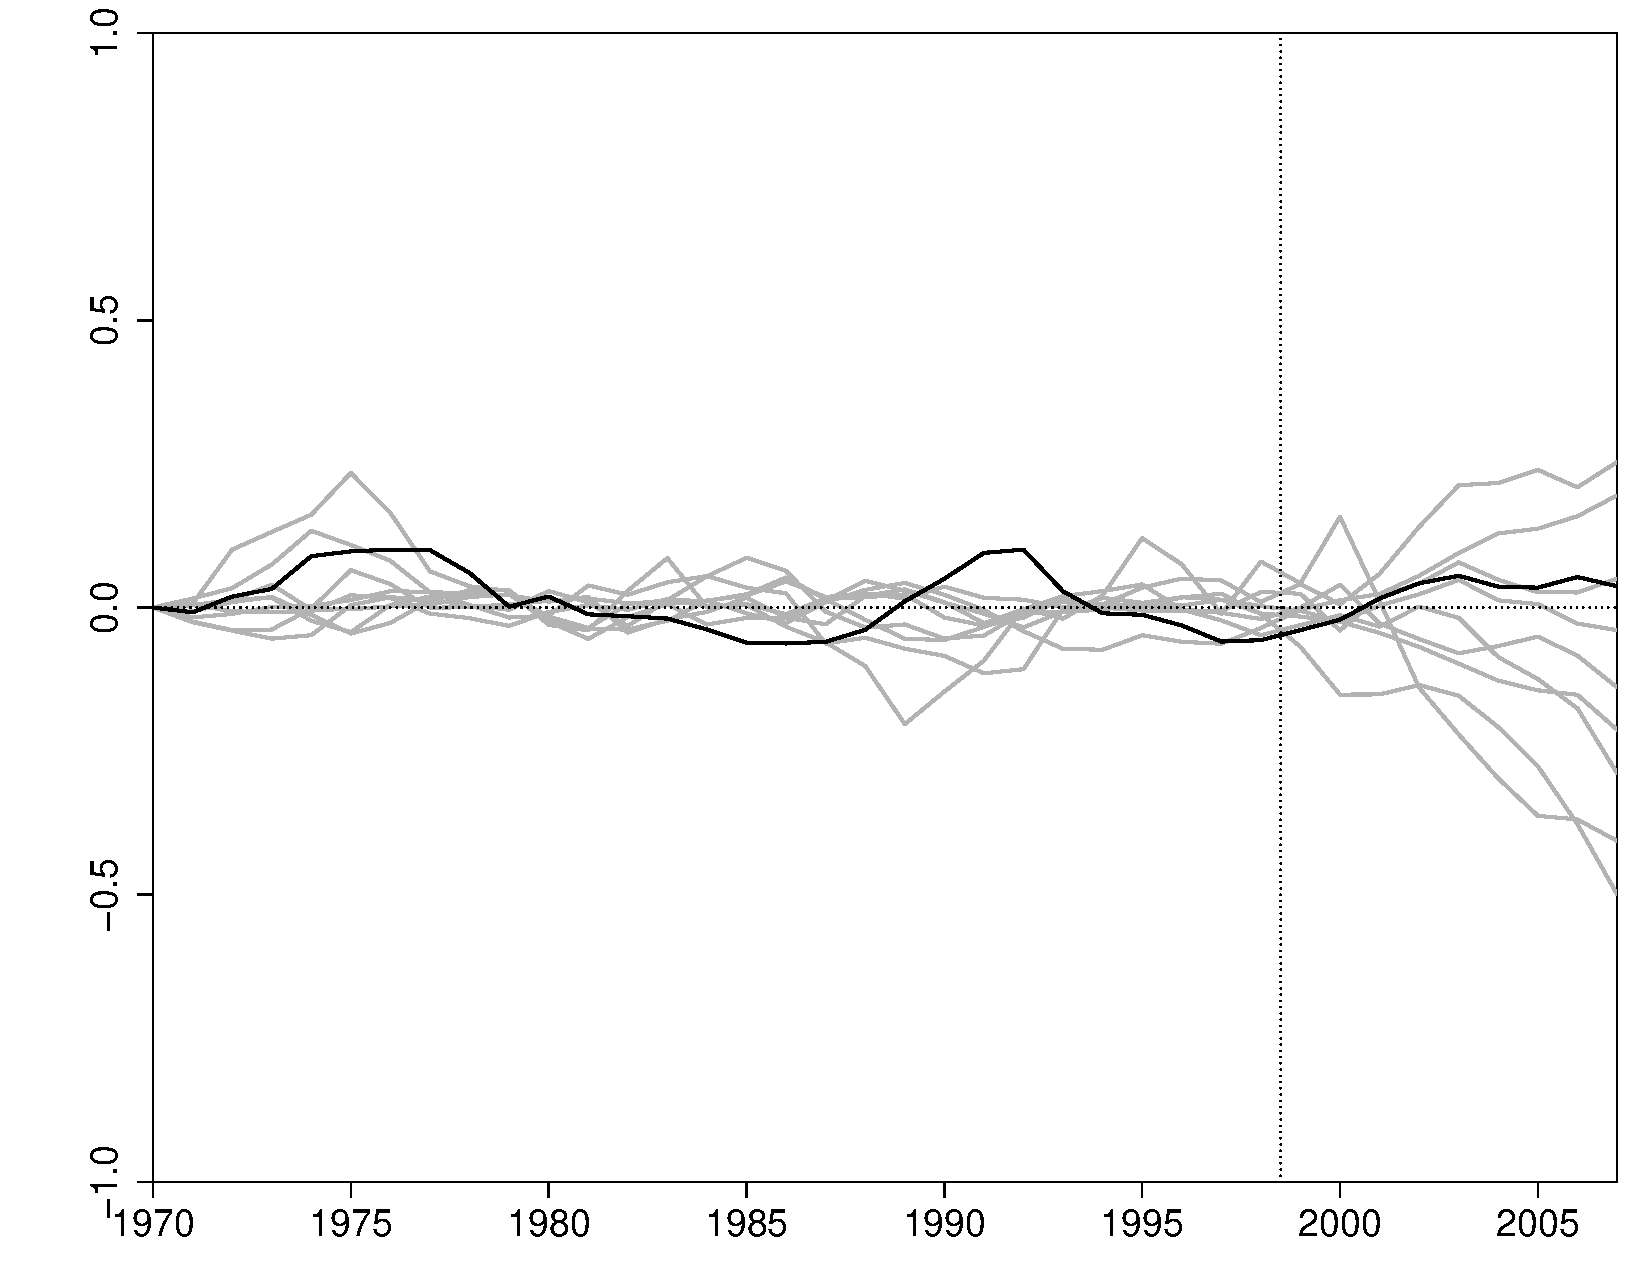
\includegraphics[width=5cm]{graph_placebo_effects_excluding_outliers_26.pdf}} \vspace{-1em}
		\annote{\footnotesize The plotted lines represent the prediction error for the treated country (black) and donor countries (grey) for which we impose a fictitious euro accession. We do not plot the donor countries whose pre-treatment MSPE was four times larger than the one of the treated country.}
\end{figure}

The plots from Figure \ref{F_Placebo} depict the doppelganger gaps for treated countries (black lines) and donor countries (grey lines), that is, the differences between each countries' normalized GDP and their doppelgangers' estimates. The smaller the gap for the pre-treatment period, the better the fit of the synthetic series to the outcome variable. Countries with a bad pre-intervention fit are excluded from the in-space placebo test because they are not suited to inform about the post-treatment effect.\footnote{We define a good pre-intervention fit following \cite{Firpo2018} when the pre-intervention MSPE of a donor country is at most four times greater than the Eurozone country’s pre-intervention MSPE being analyzed.} 

Visually, Figure \ref{F_Placebo} reinforces the findings in Figure \ref{F_1}. When comparing the full black lines from each Euro-adopter country to the grey lines of fictitious treated units, it is clear that,  for some countries, the post-treatment gap is unusually bigger. Specifically, it suggests a positive impact of the euro accession on Ireland and Luxembourg and a negative impact, if any, on France, Germany, Italy, and Portugal.

%Following \cite{Firpo2018}, I might add graphs with confidence intervals built based on this placebo test for all 12 countries.  \textbf{Figure here!}\\

\subsubsection{Statistical Significance \label{SS_stat}}

To evaluate the statistical significance of our estimates and following \cite{Abadie2010, Abadie2018}, we use a test based on the classic framework for permutation inference which builds on the computations presented in the previous section.
%\footnote{As \cite{Abadie2010} discuss, this approach produces classical randomisation inference if the intervention is indeed randomly allocated across units as we argue. If this is not the case, the approach is best interpreted as a series of placebo checks that examine whether the estimated treatment effect is large compared to the placebo effects for other flows that we would not expect to be affected by the euro adoption.} 

Given our estimates of all fictional treatment effects in the previous section, we can evaluate the statistical significance by computing a p-value associated with the treatment. First, we compute the ratio of root mean squared prediction errors (RMSPE) in the post-intervention period relative to the pre-intervention period for treated and fictitiously treated units as follows:

\begin{equation}
    \label{EQ_test}
    \chi \equiv \frac{RMSPE_{post}}{RMSPE_{pre}}  \equiv \frac{\sqrt{\frac{1}{T-T_0+1} \sum\limits_{t=T_0}^{T} (x_{1,t} - \vec{x_{0,t}} \vec{w})^2}}{\sqrt{\frac{1}{T_0-1} \sum\limits_{t=1}^{T_0-1} (x_{1,t} - \vec{x_{0,t}} \vec{w})^2}}
\end{equation}

where $x_{1,t}$ denotes the GDP of the treated country at period t; $\vec{x_{0,t}}$ denotes a vector of observations of GDP for the donor countries in period t; $\vec{w}$ denotes a vector of weights for the donor countries, $T$ denotes the total number of periods, and $T_0$ denotes the treatment date. 

This statistic already allows a quantitative analysis of the treatment effect taking into account the quality of the match produced by the SCM. A small pre-treatment RMSPE implies a good fit of the synthetic series to the actual series and a large post-treatment RMSPE suggests, for the treated units, a large intervention impact. Therefore, obtaining a larger ratio for the treated unit than for the placebo-treated units would entail a significant treatment effect.\footnote{A large post-intervention RMSPE per se is not indicative of a large effect of the intervention. It depends on whether the synthetic control can reproduce closely the outcome of interest prior to the intervention \cite{Abadie2019}.}

Figure \ref{F_RMSPE} depicts this relative measure for the Eurozone countries (black diamonds) and its donors (grey circles). Ireland clearly stands out as the country with the highest RMSPE ratio with a post-intervention gap about 16 times larger than its pre-intervention gap. 

\begin{figure}[h!]
    \centering
    \caption{\label{F_RMSPE} Ratio between the Post- and Pre-Treatment RMSPE}
    \includegraphics[scale=0.7]{RMSPE.eps}
    \annote{The plots show the ratio between the post- and the pre-intervention RMSPE for the treated units (in black diamonds) and all donor countries (in grey circles).}
\end{figure}

We deem the effect of the euro adoption significant if the estimated effect for the treated units is unusually large relative to the distribution of the placebo effects - which is the case for Germany, France, Ireland, Italy, and Portugal. To test this in practice, we follow \cite{Abadie2015} and compute a p-value which compares the value of the RMSPE for the treated country to that of all other units as follows:

\begin{equation}
\label{EQ_test2}
    \rho_1 = \sum\limits_{i=1}^{N+1} I(\chi_i \geq \chi_1) \ / \ (N+1)
\end{equation}

where $I(.)$ denotes the indicator function, $N$ the number of donor countries, $\chi_1$ the RMSPE ratio for the treated unit and $\chi_i$ is the RMSPE ratio for country \textit{i} which can be a donor or the treated country. 

Adding the information from Figure \ref{F_RMSPE} to this test definition, if one were to pick a country at random for the Irish case, the chances of obtaining a ratio as high as the Irish one would be 1 out of 15. The exact same interpretation holds for Italy. For Germany, France, and Portugal the chances of obtaining a ratio as high as their own would be 2 out of 15, which is also a sizeable effect.\footnote{For completeness, Table \ref{TA_RMSPE} presents the RMSPE ratios, ($\chi$), for all countries in the baseline analysis and the correspondent p-values for the treated units.}

\subsection{Further Robustness Checks} 

\subsubsection{Changes to Donor Pool \label{SS_donor}}

This section addresses two concerns. First, some countries in the control group may have opted out of the treatment. This would suggest a reverse causality problem and raise doubts about the credibility of the results presented. As discussed at the beginning of Section \ref{SS_Causality}, countries used in the analysis must not have opted in or out due to economic considerations. 

In fact, the UK, Sweden, and Denmark belonged to the European Union at the time but did not adopt the common currency. Even though they did opt out due to political reasons, we still address this issue by excluding these countries altogether from the donor pool.\footnote{Removing all European countries, or middle-income OECD countries like Mexico and Chile instead do not qualitatively change the robustness of the exercise.} We redo our analysis with this new pool and the results are presented in Figure \ref{F_donor}. The main conclusions remain unchanged, in particular, for the ones whose doppelgangers' construction highly relied on this trio - Austria, Belgium, France, Germany, Italy, and Portugal.
%with Ireland exhibiting a large economic gain from the euro accession.

%\footnote{According to Table 2 in \cite{Campos2018}, Sweden was not even significantly affected by joining the EU in 1995 and thus, it is not problematic to use this country in our analysis.}

\begin{figure}[h!]
    \centering
    \caption{Impact of the Euro Accession with a Change in the Donor Pool \label{F_donor}}
    \includegraphics[scale=1.2]{SCM_withoutGBRSWEDNK.eps}
    \annote{In each graph, the blue dashed line represents the normalized real GDP for the synthetic country and the black full line represents the series for the actual country. The shaded area corresponds to two standard deviations of the difference between the treated country and the doppelganger prior to the euro accession. The vertical line depicts the treatment period - 2001 for Greece and 1999 for the remaining countries. For all countries the analysis starts in 1970 and ends in 2007. Relative to the baseline analysis, the donor pool now excludes Denmark, Sweden and the United Kingdom. Table \ref{TA_weights_placebo} show the weights used to construct these results.}
\end{figure}

Second, there might have been spillover effects of the treatment on the donor countries. We address this issue by iteratively re-estimating our baseline estimate for each Eurozone country excluding in each iteration one of the countries with positive weight \citep{Abadie2015}. Moreover, this robustness check also tests the hypothesis that a single country in the donor pool biased the results. If the exclusion of a single unit from the donor pool has a large effect on results--without a discernible change in pre-intervention fit--the estimated results might be caused by other interventions or by particularly idiosyncratic shocks on the outcome of the excluded untreated unit.

We display this robustness check for countries that weighted, at least, 10\% in the construction of, at least, 2 countries' counterfactuals in Appendix \ref{SS_donor_appendix}. This exercise shows that no particular donor country is driving the main conclusions. So, it is unlikely that there were spillover effects of the treatment on the donors or that one specific country in the donor pool is driving the results.\footnote{The robustness of SCM comes exactly from having similar results using different donors, even if the estimated weights change.}
%\footnote{For the sake of brevity, the figures for all the remaining countries are not reported, but they can be provided by the authors upon request. The results remain qualitatively unchanged.} So, it is unlikely that spillover effects nor one specific country in the donor pool are driving the results.

\subsubsection{Changes in the Sample Period \label{SS_start}}

The credibility of the SCM results severely depends on whether the requirements specified in Section \ref{SS_Implementation} are satisfied. One of these requirements was that countries should not experience differentiated shocks during the sample period. Several analysed countries joined the European Union during the pre-treatment period may concern the most attentive reader. 

For countries that joined the EU at least 10 years before the Eurozone creation, we re-do the estimates using their accession data as the start of our sample, that is, Ireland (1973), Greece (1981), Portugal, and Spain (1986). From Figure \ref{F_Start}, it is possible to conclude that the results from the baseline analysis are robust.

\begin{figure}[h!]
	\centering
	\caption{The Impact of the Euro Accession with a Change in the Sample Period}	
	\label{F_Start}
    \subfigure{\includegraphics[width=7cm]{Ireland_1973.eps}}
    \subfigure{\includegraphics[width=7cm]{Greece_1981.eps}}
    \subfigure{\includegraphics[width=7cm]{Portugal_1986.eps}}
    \subfigure{\includegraphics[width=7cm]{Spain_1986.eps}}
    \vspace{-1em}
	\annote{In each graph, the blue dashed line represents the normalized real GDP for the synthetic country and the black full line represents the series for the actual country. The shaded area corresponds to two standard deviations of the difference between the treated country and the doppelganger prior to the euro accession. The vertical line depicts the treatment period - 1999 for Ireland, Greece, and Portugal and 2001 for Greece. The analysis starts in 1973 for Ireland, 1981 for Greece, and 1986 for Portugal and Spain. For all countries, the analysis ends in 2007.
    }
\end{figure}

Unfortunately, it is not possible to re-estimate the results for Austria and Finland because they joined the EU in 1995. Yet, according to \cite{Campos2018}, Austria and Finland were not significantly affected by the EU accession and thus we believe that this does not pose a problem to our analysis.


\section{Unpacking the GDP gap \label{S_Components}}

In this section, we take one step further and inspect the results presented in Figure \ref{F_1} by decomposing the euro accession response of GDP into the response of its components. First, we compute the series for each GDP component for both countries and corresponding counterfactuals. Then, we uncover which components were positively or negatively affected and account for the output gains and losses from the accession. 

This analysis begins by constructing the synthetic shares of GDP components using the weights estimated in Section \ref{S_Doppelganger} and the data from the donor countries. We use the weights previously computed to be able to directly decompose the GDP and also to avoid over-fitting when using this method.

Similarly to the construction of the synthetic GDP series, we now compute the synthetic shares of each GDP component as a weighted average of the shares of GDP components for the donor countries. To be precise, we thus obtain GDP shares of private consumption, investment, government consumption, exports, and imports. Then, we use each component share and the GDP series to compute the five GDP components series for both countries and doppelgangers. In Appendix \ref{SS_Components}, we present these series as a deviation from the 1970 value in percent.

It is important to highlight that comparing the actual and the synthetic series from Appendix \ref{SS_Components} also indicates whether the doppelganger can really mimic the behaviour of each country prior to the euro accession. We must recall that the construction of the doppelganger in Section \ref{S_Doppelganger} only targets the average and not the time path of GDP components and thus, a good fit in this regard can not be taken for granted. Overall, the figures from Appendix \ref{SS_Components} reassure us of the good fit of our estimates with the majority of the series lying inside the two standard deviations band in the pre-treatment period. 

%\subsection{What explains the cumulative doppelganger gap?}

Next, we compute the contribution of each GDP component for the output gap generated by the treatment. In section \ref{SS_Method}, Equation \ref{EQ_objective} defines the doppelganger gap as the difference in the outcome variable (here, real GDP) between the treated and the synthetic country. The cumulative treatment effect can be estimated by computing the doppelganger gap for $t=2007$, the last year of our analysis.
%In this section, we compute doppelganger gaps for the GDP $ = GDP_{t,c}-GDP_{t,c}^{dop} = x_{1,t} - \vec{x_{0,t}} \vec{w} $.     

Here, we proceed in four steps. Analogously to Equation \ref{EQ_objective}, we start by computing doppelganger gaps for each GDP component. Then, we compute the relative weight of each component $z$ on the output doppelganger gap in the following way:

\begin{equation}
\label{equation2}
\text{weight of \textit{z}}_{c,t}= \frac{z_{c,t} - z_{c,t}^{dop}}{GDP_{c,t} - GDP_{c,t}^{dop}}
\end{equation}

where \textit{z} is either private consumption, government consumption, investment, exports, or imports, the subscript \textit{c} stands for one of the twelve treated countries, and the subscript \textit{t} represents the time period. Thereafter, we calculate the \textbf{percent} doppelganger gap for GDP as follows:

\begin{equation}
\label{equation3}
\text{percent output doppelganger gap }_{c,t}= \frac{GDP_{c,t}-GDP_{c,t}^{dop}}{GDP_{c,t}^{dop}}
\end{equation}

Showing the treatment effect in percent terms allows a direct interpretation of how much larger/smaller the GDP is due to the euro accession. Finally, we multiply the relative weight of each doppelganger gap $z_{c,t}$ by the percent output doppelganger gap. This allows us to understand the direct contribution of each channel to the treatment effect.

Figure \ref{F_Decomposition} depicts, for each country, the percent GDP gap in 2007 and its decomposition. It clearly shows that countries experienced the euro accession heterogeneously.\footnote{See Table \ref{T_Decomposition} for the exact values depicted in Figure \ref{F_Decomposition}.}  

%Then, Figure \ref{} shows the whole evolution of the percent output gap and respective component contributions. 
\begin{figure}[h!]
    \centering
    \caption{Doppelganger Gaps and GDP Components}
    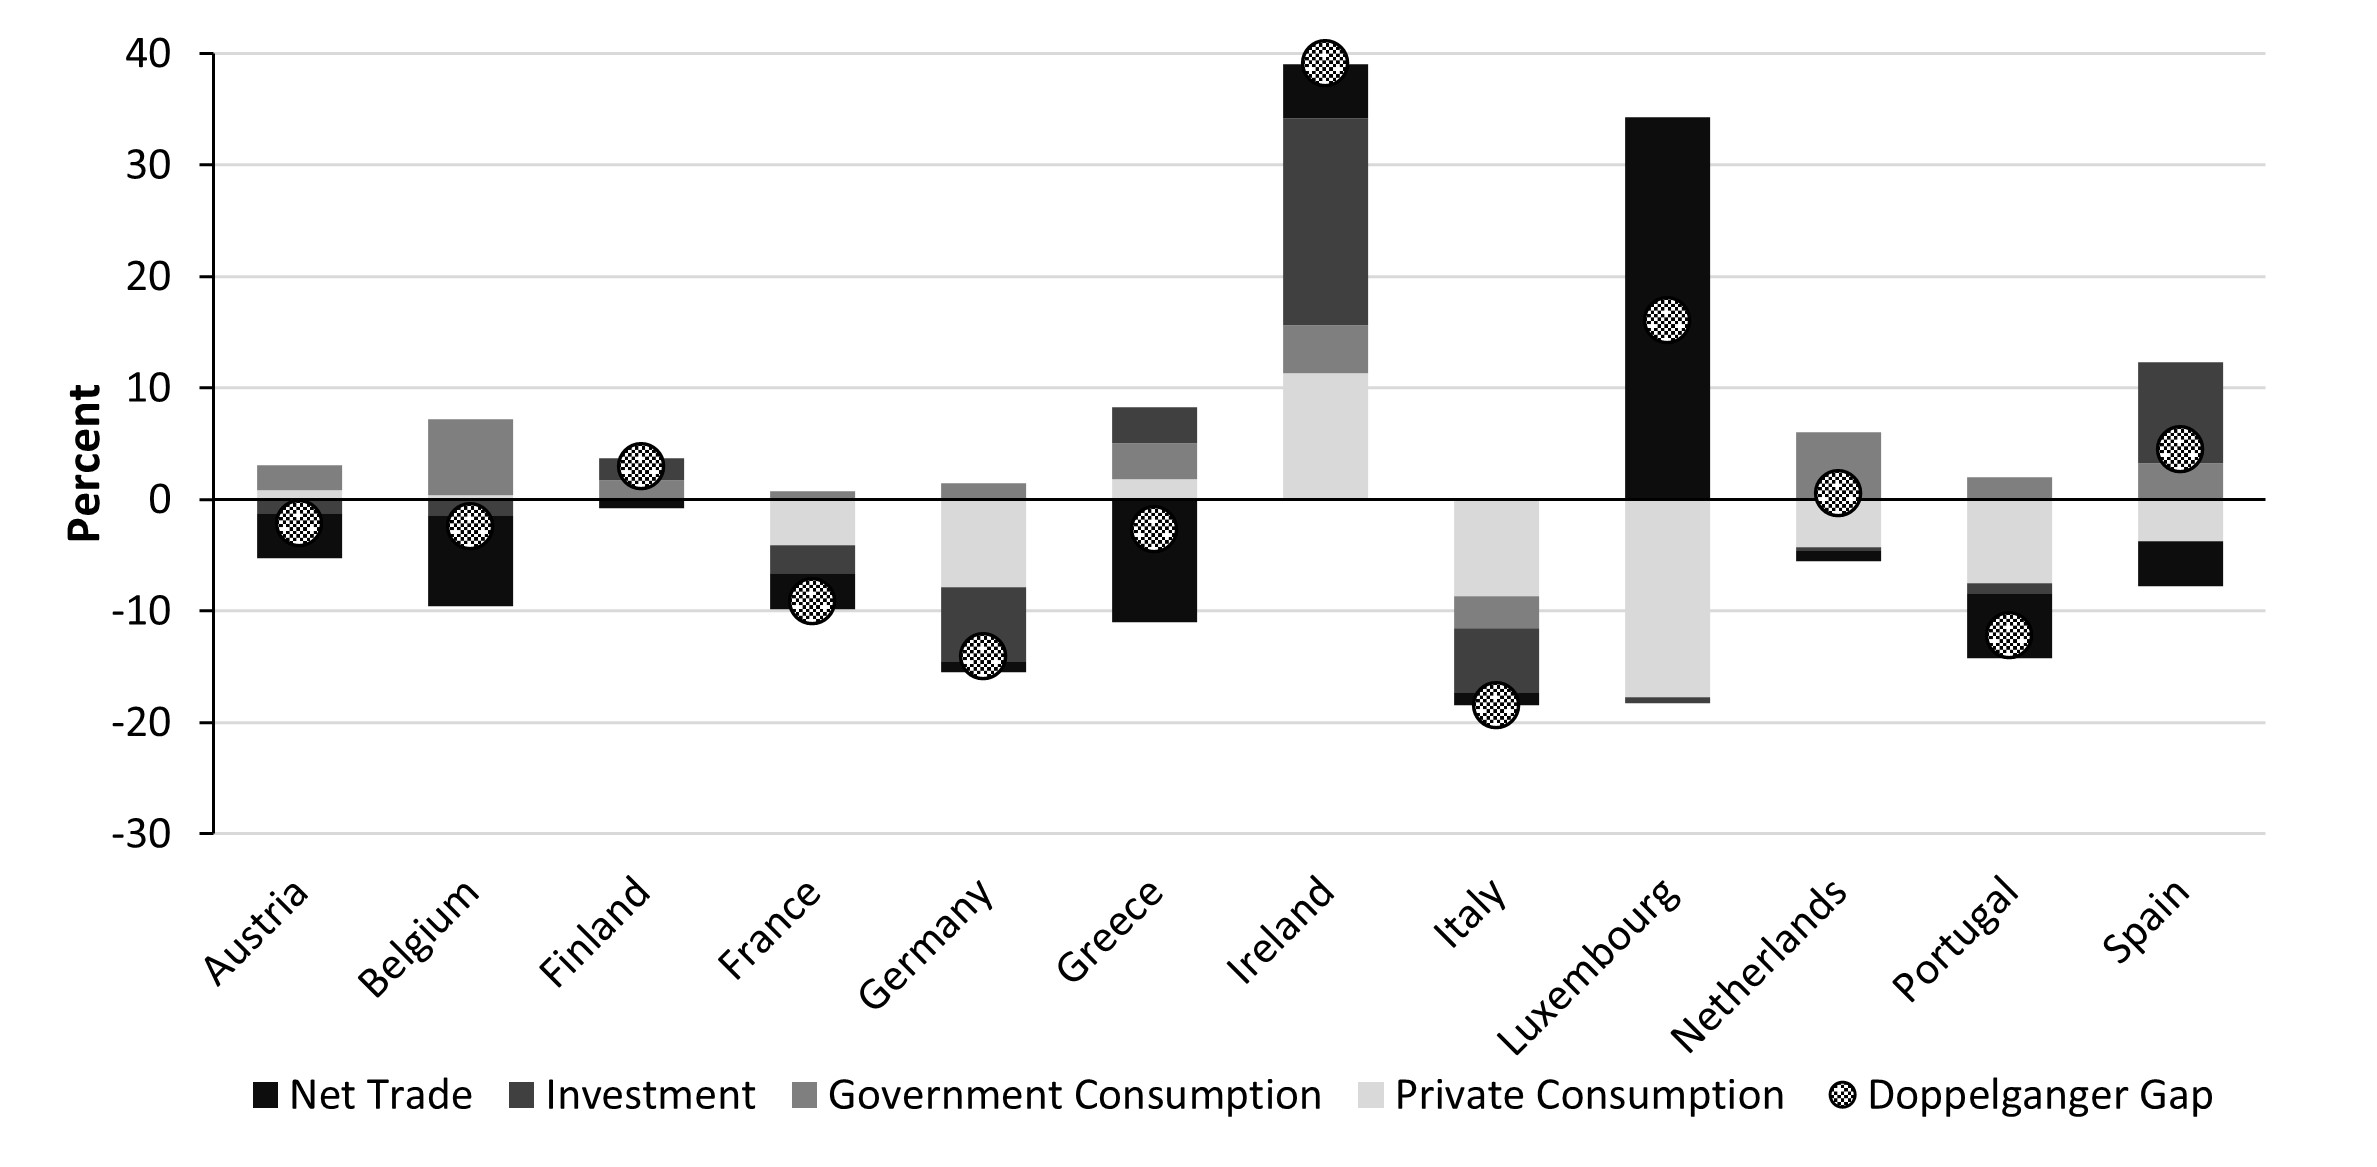
\includegraphics[scale=0.8]{Decomposition.jpg}
    \annote{The dot depicts, for each country, the percent  doppelganger gap of output computed as in Equation \ref{equation3}. The stacked bars represent the contribution of each GDP component for these gaps. The values for GDP component sum up the percent doppelganger gap for each treated unit. The values represent the cumulative effect of the euro accession since they are computed for 2007, the last year of the analysis.}
    \label{F_Decomposition}
\end{figure}

\textbf{Countries that implemented spending-based austerity measures between 1992 and 1998} Austria, Belgium, Germany, Spain, Finland, France, Italy

\textbf{Countries that did not implement spending-based austerity measures between 1999 and 2007} Austria, Belgium, Spain, Finland, France,

Italy and Portugal did implement strong austerity measures between 2004 and 2006 accounting for more than 3\% of GDP in total for each country.

We now take a deeper look into the countries which were significantly affected as argued in Section \ref{SS_Causality}. For Ireland, joining the Eurozone boosted GDP by 39\%. Even though all GDP components contribute positively to this result, the private consumption and investment together can explain almost 80\% of the total output gain from the treatment.

Table \ref{T_Decomposition} also shows that the reasons behind the economic slowdown experienced by some countries at the euro accession differ from country to country. We find that for France and Portugal, the private consumption and the net exports accounted for a large share of the GDP gap. For Germany and Italy, it is the doppelganger difference in private consumption alongside investment that better explains the negative economic impact of the euro on GDP.

For most countries, government consumption is one of the components with a positive contribution. On the one hand, this is a puzzling finding given the Eurozone countries were operating under the fiscal rules of the Stability and Growth Pact (SGP) during the post-treatment period.\footnote{Nevertheless, according to \cite{Bofinger2003}, the correlation between the average real growth rate of government consumption and fiscal deficits between 1999 and 2002 was negative, meaning that the low deficit rules did not necessarily imply less government spending.} 

On the other hand, before the Euro accession, there were stringent Maastricht convergence criteria which might have restricted government consumption, creating then more fiscal space after 1999. There seems to be indeed a strong negative relationship between the fiscal spending before and after the Euro adoption. Most countries in the sample, like Finland and Spain, implemented spending-based austerity measures after the Maastricht Treaty in line with the Stability and Growth Pact (SGP) \citep{Alesina2019}.\footnote{Countries that implemented spending-based austerity measures between 1992 and 1998 were Austria, Belgium, Germany, Spain, Finland, France, and Italy. Countries that did not implement spending-based austerity measures between 1999 and 2007 were Austria, Belgium, Spain, Finland, and France.} This has likely created fiscal space which together with access to cheaper credit promoted an increase in government consumption beyond what would have happened absent the Euro adoption. Other countries, such as Portugal, that did not consolidate spending before the Euro accession, also did not boost government consumption afterwards. 

Before the Euro, the need to exchange local currencies implied extra transaction costs and exchange rate risk. The single currency was expected to boost cross-border trade and investment between the member states since doing business in the Eurozone would be more cost-efficient and less risky \cite{DeGrauwe2020}. For third parties, the Eurozone would be an attractive place to invest as well. Consumers would benefit from price transparency and stability. Therefore, it would be expected an increase in investment, exports, and imports but it is not clear in which direction the trade balance would go.

Table \ref{T_Decomposition_NX} indeed reveals that, except for France and Italy, all countries had a higher trade volume than if they had not adopted the common currency. This result is in accordance with \cite{Baldwin2008} and \cite{Schmitz2011} who argue that the euro has significantly promoted trade in the Eurozone countries. Yet, net exports changed differently across countries. Only Germany and Ireland experienced significant net trade benefits from the euro accession. We corroborate the negative impact on net exports in most cases as documented in \cite{Hope2016}. 

Moreover, even though the common currency was expected to attract foreign investment for the whole Eurozone, Ireland stands out from the remaining member countries. Investment in Ireland increased significantly because of the euro adoption. Therefore, country-specific characteristics have significantly shaped the impact across member states.   

% \subsection{What happened after the Maastricht Treaty might help us understand some of the dynamics we see after the Euro adoption.}

% \begin{figure}[h!]
%     \centering
%     \caption{Doppelganger Gaps and GDP Components}
%     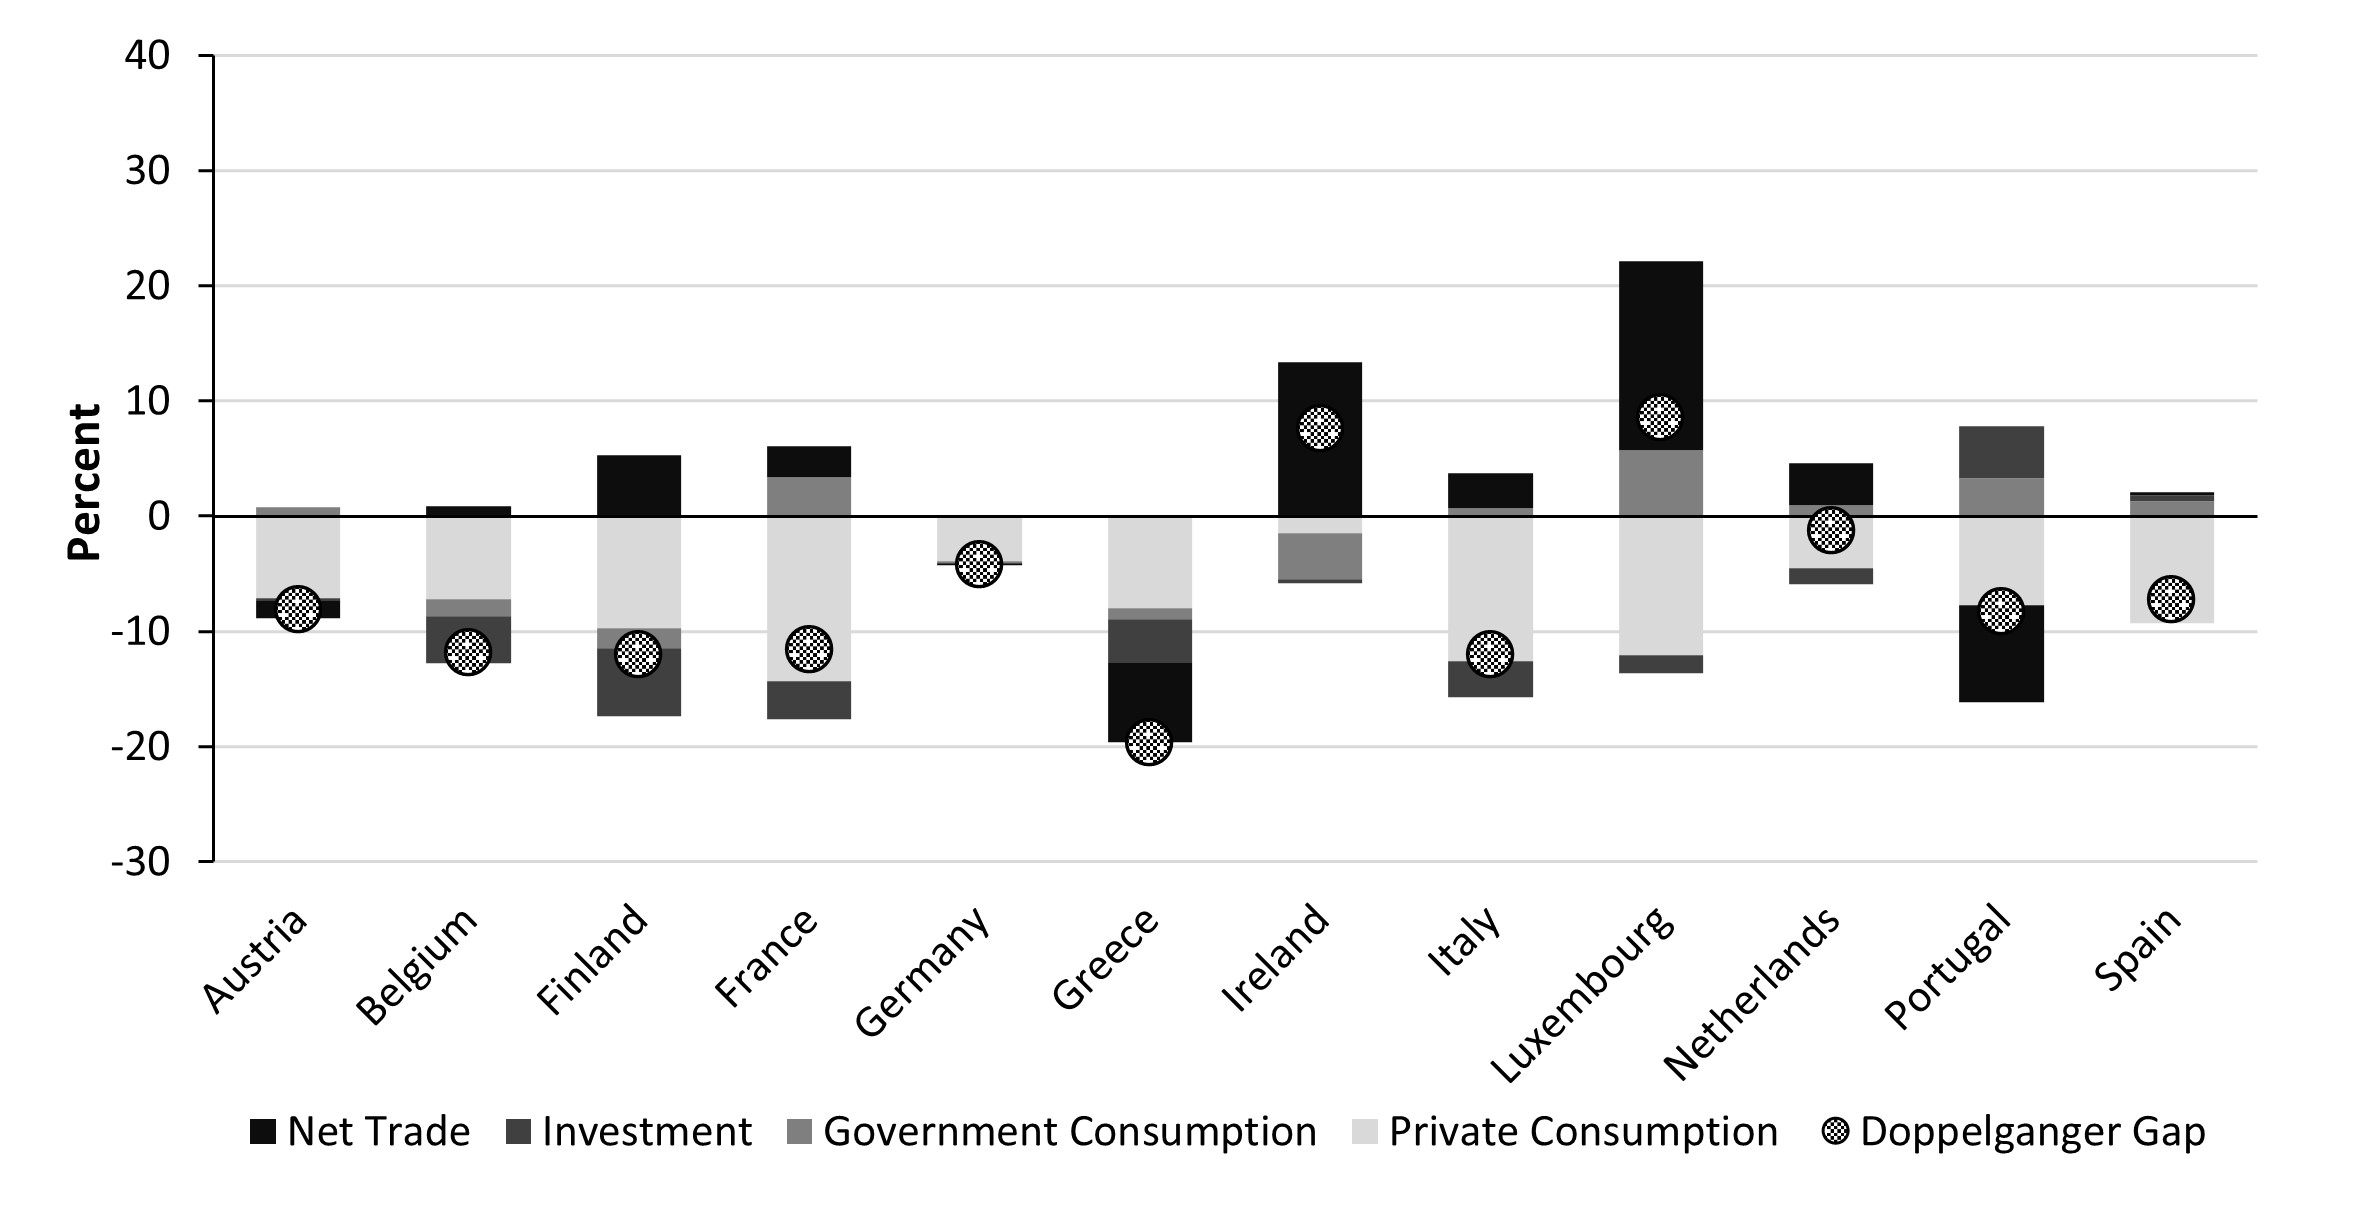
\includegraphics[scale=0.8]{Decomposition_1999.jpg}
%     \annote{The dot depicts, for each country, the percent doppelganger gap of output computed as in Equation \ref{equation3}. The stacked bars represent the contribution of each GDP component for these gaps. The values for GDP component sum up the percent doppelganger gap for each treated unit. The values represent the cumulative effect of the euro accession since they are computed for 2007, the last year of the analysis.}
%     \label{F_Decomposition_1999}
% \end{figure}

\section{Did Euro Area Nationals Gain with the Euro Adoption? \label{S_GNI}}

GDP and Gross National Income (GNI) are both important measures to gauge the economic performance of a country. GDP measures the total value of all goods and services produced in a country, focusing on the output generated by the factors of production within the country, regardless of the nationality of the owners. It thus includes the output of foreign-owned firms operating within the country's borders but excludes the output of domestic-owned firms operating abroad. GNI, on the other hand, measures the total income earned by a country's residents, regardless of where they are located geographically. It includes GDP plus any income earned from abroad by residents of the country, excluding income earned domestically by foreign residents. 

Given the important role of profits and income earned by foreign companies operating domestically for some Euro adopters (e.g., Ireland), we extend the analysis to use GNI as an outcome variable. Figure \ref{F_GNI} shows the results.\footnote{Due to data limitations, Greece and some donor countries are excluded from this exercise.} Ireland's economic gains from the Euro adoption are still positive when measured by GNI, meaning that total income earned by residents increased amid the Euro adoption. However, the gains are considerably smaller than when using GDP. For other countries, results remained broadly unchanged albeit with poor pre-treatment fit. 

Ireland has become an attractive destination for high-growth companies and global corporations due to its favorable corporate tax environment, skilled workforce, and membership in the European Union.\footnote{Following the Government's announcement in July 1998 to introduce a standard rate of corporation tax of 12.5\% for trading income with effect from 1st January 2003, the Government has commenced the process of reducing the existing standard rate of corporation tax. Ireland's corporate tax rate of 12.5\% is among the lowest in Europe, which has been a significant factor in attracting multinational companies.}
While the activities of these multinational corporations contribute significantly to Ireland's GDP through production and services rendered within the country, a large portion of the profits are repatriated to foreign investors or parent companies. This implies that although these profits count towards Ireland's GDP, they do not contribute to Ireland's GNI.



\begin{figure}[h!]
    \centering
    \caption{The Impact of the Eurozone Accession - Gross National Income per capita}
    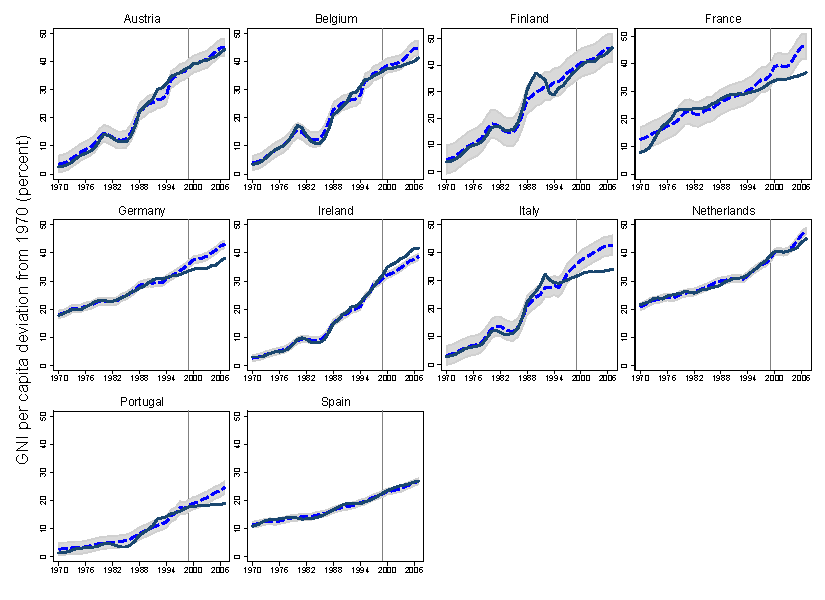
\includegraphics[width=\textwidth]{Output/Figures/SCM_gnipc_Annual.pdf}
    \annote{In each graph, the dashed line represents the inflation rate for the synthetic country and the continuous line represents the series for the actual country. The shaded area corresponds to two standard deviations of the difference between the treated country and the doppelganger before the euro accession. The vertical line represents the treatment period - 1999 for all countries except for Greece which is 2001. For each country, the analysis starts in 1970 and ends in 2007.}
    \label{F_GNI}
\end{figure}


\section{Conclusion \label{S_Conclusion}}
In this paper, we study the impact of the EMU accession on the macroeconomic performance of the first twelve member states. We use the synthetic control method to construct a counterfactual of these countries' GDP. This method allows building a doppelganger that should represent the economic activity of these countries in the absence of the euro adoption. 

Our findings suggest that there are mild losers (France, Germany, Italy, and Portugal) and a clear winner (Ireland). Notwithstanding, the drivers of such estimates are heterogeneous.  First, Ireland's economic gains are more modest when excluding profits and income earned by foreigners, while the results remain unchanged for other countries. Second,  our GDP decomposition analysis indicates that for the majority of Eurozone countries, the euro spurred government consumption, while deterring investment and private consumption. The common currency also stimulated trade in most cases but only Germany, Luxembourg, and Ireland bear positive net trade benefits.  

This evidence points out the importance of analyzing in detail the heterogeneous responses of GDP components and their implications. For example, given the different responses of investment and government consumption across member states, it is natural to ask if the effectiveness of national fiscal policies has changed. This could be especially interesting given that, with the common currency adoption, countries forgo important policy instruments.


%\section*{Declaration}
%On behalf of all authors, the corresponding author states that there is no conflict of interest.

%\section*{Acknowledgements}
%We thank Benjamin Born, Evi Pappa, David Hope, Donghai Zhang, Laura Puzzello, Martin Kornejew, Moritz Schularick, Pedro Gomis-Porqueras, Vitor Possebom as well as Paola Boel and the remaining research division members at the Sveriges Riksbank for their feedback and discussions. We likewise thank seminar participants at the University of Bonn and participants of the $13^{th}$ Annual Meeting of the Portuguese Economic Journal. We would like to thank the Sveriges Riksbank for hosting us while conducting part of the research that led to this paper. We acknowledge financial support from from the Fundação para a Ciência e Tecnologia [projects references SFRH/BD/144581/2019 and SFRH/BD/144820/2019] the Deutsche Forschungsgemeinschaft (German Research Foundation) under Germany's Excellence Strategy [EXC 2126/1 - 390838866] and under the RTG 2281 - The Macroeconomics of Inequality.

\clearpage
\singlespace
\bibliographystyle{chicago}
\bibliography{Bibliography}

\clearpage

\begin{appendices}

\setcounter{page}{1}
\setcounter{table}{0}
\setcounter{figure}{0}
\renewcommand{\thepage}{\roman{page}}
\renewcommand{\thetable}{\Alph{section}.\arabic{table}}
\renewcommand{\thefigure}{\Alph{section}.\arabic{figure}}
\renewcommand{\theEquation}{\Alph{section}.\arabic{Equation}}

\begin{titlepage}

\begin{center}
\textbf{\huge{Adopting the Euro: a Synthetic Control Approach}}\\

\vspace{4em}

\textbf{\huge{Online Appendix}}\\

\end{center}

\thispagestyle{empty}
%\maketitle

\end{titlepage}


\section{Appendix}
\subsection{Variables Description and Source}
\begin{table}[!htbp] 
\centering
\footnotesize
\caption{\label{TA_Description} Variables Description}\centering\medskip
\begin{tabular}{p{2cm}p{9cm}p{3.5cm}}
\hline
%rgdpna rconna rdana rnna wa_pop_s emp pop
 Variable code & Description & Source \\ 
 \hline \hline
 rgdpna & Real gross domestic product at constant 2011 national prices in million 2011 US dollars normalized to unity in 1970. & PWT 9.1 \\ \hline
 %rconna & Real consumption at constant 2011 national prices in million 2011 US dollars.  & PWT 9.1 \\ \hline
 %rdana & Real domestic absorption at constant 2011 national prices in million 2011 US dollars.  & PWT 9.1 \\ \hline
 %rinvna & Investment at constant 2011 national prices in million 2011 US dollars computed by subtracting rconna to rdana. & PWT 9.1 \\ \hline
 %rnxna & Net exports of goods and services at constant 2011 national prices in million 2011 US dollars computed by subtracting rdana to rgdpna & PWT 9.1 \\ \hline
 %rgovna & Real government consumption at constant 2011 national prices in million 2011 US dollars. In order to compute this variable one needs to use the share of government consumption in current PPPs (csh\_g) to obtain a series for government consumption in current PPPS cgovn=((csh\_g/(csh\_g+csh\_c))*ccon). Then, in order to adjust for constant PPPs obtain the deflator of total consumption (rconna/ccon) and multiply it by cgovn. & PWT 9.1 \\ \hline
 pop & Total population in millions. & PWT 9.1  \\ \hline
 rgdpnapc & Per head real gross domestic product at constant 2011 national prices in 2011 US dollars computed by dividing rgdpna by pop normalized to unity in 1970. & PWT 9.1 \\ \hline
 rgdpepc & Per head (expenditure side) real gross domestic product at chained PPPs 2011 US dollars computed by dividing rgdpe by pop normalized to unity in 1970. & PWT 9.1 \\ \hline
 emp & Total employment - number of persons engaged in millions. & PWT 9.1\\ \hline
 csh\_prod & Labor productivity growth computed by taking the log-difference between real gdp and total employment & PWT 9.1 \\ \hline
 csh\_emp & Employment share - ratio between total employment and total population & PWT 9.1 \\ \hline
 csh\_c & Private consumption expenditure (\% of GDP) obtained by subtracting general government final consumption expenditure to the series of final consumption expenditure & World Bank \\ \hline
 csh\_g & General government final consumption expenditure (\% of GDP) & World Bank \\ \hline
 csh\_i & Gross fixed capital formation (\% of GDP) & World Bank \\ \hline
 csh\_x & Exports of goods and services (\% of GDP) & World Bank \\ \hline
 csh\_m & Imports of goods and services (\% of GDP) & World Bank \\ \hline
 gnipc &  Gross national income per capita & World Bank \\ \hline
 inflation & Inflation rate (\%), Counsumer Price Index of All Commodities& IMF IFS \\ \hline
 Bonds & Long-Term Government Bond Yields, Percent per annum & \cite{Arvai2023} \\ \hline
 %unemp  & Unemployment Rate (\%)                    & World Bank \\ \hline
 
 \hline 
\end{tabular}
\annote{All variables collected directly from the Penn World Table are from version 9.1 (PWT 9.1) \cite{Feenstra2015}. All level variables are in real terms and at annual frequency spanning the year 1970 until 2007. GDP components were collected from the World Bank database in shares of GDP. IMF IFS stands for the International Monetary Fund, International Financial Statistics (IFS) database.}
\end{table}

\clearpage
%\subsection{Descriptive Statistics}
\subsection{Comparison Tables}

\vspace{-1.5em}

\begin{center}
\footnotesize
\begin{longtable}{lcc}
\caption{\label{TA_comp} Predictors' Means (in \%) during Pre-Treatment Period}\\
\hline  
\hline  
 \multicolumn{1}{c}{\textbf{Variable Names}}   & \textbf{Country}  & \textbf{Doppelganger}  \\
\hline 
 \endfirsthead
\multicolumn{3}{l}{\emph{... table \thetable{} continued}} \\
\hline \hline 
 \multicolumn{1}{c}{\textbf{Variable Names}}   & \textbf{Country}  & \textbf{Doppelganger}  \\
\hline
\endhead
\hline
\multicolumn{3}{r}{\emph{Continued on next page...}}\\
\endfoot
\endlastfoot
\textbf{Austria} &  &  \\  
Share of Priv. Consumption &     56.27 &     54.58 \\  
Share of Investment &     26.53 &     26.02 \\  
Share of Gov. Consumption &     17.91 &     17.39 \\  
Share of Imports &     32.57 &     35.93 \\  
Share of Exports &     31.85 &     33.92 \\  
Employment Share &     45.16 &     48.31 \\  
Labor productivity growth &      2.32 &      1.35 \\  
Inflation Rate &      4.24 &      5.16 \\    \hline
\textbf{Belgium} &  &  \\  
Share of Priv. Consumption &     54.14 &     54.45 \\  
Share of Investment &     22.87 &     28.49 \\  
Share of Gov. Consumption &     21.41 &     14.42 \\  
Share of Imports &     53.80 &     41.32 \\  
Share of Exports &     55.39 &     38.67 \\  
Employment Share &     38.01 &     50.64 \\  
Labor productivity growth &      2.19 &      1.46 \\  
Inflation Rate &      4.85 &      4.84 \\  \hline
\textbf{Finland} &  &  \\  
Share of Priv. Consumption &     52.51 &     50.11 \\  
Share of Investment &     26.66 &     26.39 \\  
Share of Gov. Consumption &     19.38 &     21.69 \\  
Share of Imports &     26.57 &     33.64 \\  
Share of Exports &     28.02 &     31.84 \\  
Employment Share &     47.26 &     48.27 \\  
Labor productivity growth &      2.99 &      2.16 \\  
Inflation Rate &      6.73 &      6.72 \\    \hline
\textbf{France} &  &  \\  
Share of Priv. Consumption &     55.16 &     55.17 \\  
Share of Investment &     23.11 &     23.08 \\  
Share of Gov. Consumption &     21.24 &     20.72 \\  
Share of Imports &     20.54 &     24.69 \\  
Share of Exports &     21.03 &     23.66 \\  
Employment Share &     40.49 &     44.51 \\  
Labor productivity growth &      2.11 &      1.15 \\  
Inflation Rate &      6.22 &     11.59 \\   \hline
\textbf{Germany} &  &  \\  
Share of Priv. Consumption &     57.15 &     58.33 \\  
Share of Investment &     24.50 &     25.60 \\  
Share of Gov. Consumption &     19.68 &     14.79 \\  
Share of Imports &     21.40 &     31.43 \\  
Share of Exports &     20.06 &     30.15 \\  
Employment Share &     48.36 &     49.07 \\  
Labor productivity growth &      2.35 &      1.03 \\  
Inflation Rate &      3.54 &      4.54 \\  \hline
\textbf{Greece} &  &  \\  
Share of Priv. Consumption &     63.06 &     62.61 \\  
Share of Investment &     26.46 &     22.01 \\  
Share of Gov. Consumption &     16.75 &     15.77 \\  
Share of Imports &     21.77 &     23.49 \\  
Share of Exports &     15.50 &     23.87 \\  
Employment Share &     38.77 &     41.82 \\  
Labor productivity growth &      1.44 &      0.97 \\  
Inflation Rate &     14.70 &     15.28 \\    \hline
\textbf{Ireland} &  &  \\  
Share of Priv. Consumption &     61.17 &     55.84 \\  
Share of Investment &     21.65 &     25.10 \\  
Share of Gov. Consumption &     18.72 &     19.06 \\  
Share of Imports &     52.85 &     32.05 \\  
Share of Exports &     51.30 &     32.05 \\  
Employment Share &     35.36 &     40.78 \\  
Labor productivity growth &      3.44 &      2.28 \\  
Inflation Rate &      8.36 &     33.46 \\   \hline
\textbf{Italy} &  &  \\  
Share of Priv. Consumption &     59.00 &     62.10 \\  
Share of Investment &     22.87 &     22.38 \\  
Share of Gov. Consumption &     17.55 &     16.95 \\  
Share of Imports &     19.28 &     19.64 \\  
Share of Exports &     19.86 &     21.07 \\  
Employment Share &     38.25 &     42.35 \\  
Labor productivity growth &      2.16 &      1.56 \\  
Inflation Rate &      9.48 &     11.20 \\  \hline
\textbf{Luxembourg} &  &  \\  
Share of Priv. Consumption &     48.16 &     57.18 \\  
Share of Investment &     22.57 &     28.27 \\  
Share of Gov. Consumption &     15.33 &     14.76 \\  
Share of Imports &     81.83 &     39.39 \\  
Share of Exports &     95.78 &     39.60 \\  
Employment Share &     46.63 &     49.28 \\  
Labor productivity growth &      1.91 &      1.42 \\  
Inflation Rate &      4.61 &     14.66 \\   \hline
\textbf{The Netherlands} &  &  \\  
Share of Priv. Consumption &     50.90 &     54.78 \\  
Share of Investment &     22.62 &     26.16 \\  
Share of Gov. Consumption &     21.94 &     18.40 \\  
Share of Imports &     47.47 &     38.27 \\  
Share of Exports &     52.01 &     37.62 \\  
Employment Share &     43.78 &     49.70 \\  
Labor productivity growth &      1.45 &      1.40 \\  
Inflation Rate &      4.18 &     12.26  \\  \hline
\textbf{Portugal} &  &  \\  
Share of Priv. Consumption &     66.93 &     64.53 \\  
Share of Investment &     26.93 &     21.90 \\  
Share of Gov. Consumption &     14.03 &     15.06 \\  
Share of Imports &     31.16 &     22.84 \\  
Share of Exports &     23.27 &     24.34 \\  
Employment Share &     41.81 &     41.35 \\  
Labor productivity growth &      1.95 &      1.75 \\  
Inflation Rate &     14.14 &     14.12 \\   \hline
\textbf{Spain} &  &  \\  
Share of Priv. Consumption &     63.12 &     65.77 \\  
Share of Investment &     23.78 &     20.50 \\  
Share of Gov. Consumption &     14.51 &     15.36 \\  
Share of Imports &     18.55 &     20.84 \\  
Share of Exports &     17.13 &     22.47 \\  
Employment Share &     35.38 &     39.80 \\  
Labor productivity growth &      2.55 &      1.44 \\  
Inflation Rate &      9.87 &     16.90 \\  \hline
\hline \hline 
\end{longtable} 
\annote{Predictors' means for each country and its doppelgangers during the pre-treatment period. The doppelganger column corresponds to a simple (non-weighted) average and thus some discrepancies may arise because of that. All numbers are in percent. Variables definitions can be found in Table \ref{TA_Description}.}
\end{center}



\clearpage
\begin{landscape}
\subsection{Weights Table}
\begin{table}[htbp]
\scriptsize
\caption{\label{TA_weights} Composition of the Doppelgangers: Country Weights (in \%)}\centering\medskip
\begin{tabular}{lcccccccccccc} \toprule
\textit{Donor countries} & Austria  & Belgium  & Finland  & France  & Germany  & Greece  & Ireland  & Italy  & Luxembourg  & Netherlands  & Portugal  & Spain  \\  \midrule
Australia &       $<0.1$ &       $<0.1$ &       $<0.1$ &       $<0.1$ &       $<0.1$ &       $<0.1$ &       $<0.1$ &       26.7 &       $<0.1$ &       $<0.1$ &       $<0.1$ &       $<0.1$ \\  
Canada &       36.5 &       $<0.1$ &       $<0.1$ &       30.7 &       25.5 &       $<0.1$ &       $<0.1$ &       8.7 &       $<0.1$ &       $<0.1$ &       $<0.1$ &       $<0.1$ \\  
Chile &        $<0.1$ &       $<0.1$ &       $<0.1$ &       $<0.1$ &       $<0.1$ &       0.4 &      29.0 &       $<0.1$ &       $<0.1$ &      $<0.1$ &       $<0.1$ &       $<0.1$ \\  
Denmark &       $<0.1$ &       $<0.1$ &       $<0.1$ &       $<0.1$ &      $<0.1$ &       $<0.1$ &       $<0.1$ &       $<0.1$ &       $<0.1$ &       26.4 &       $<0.1$ &       $<0.1$ \\  
Iceland &       $<0.1$ &       $<0.1$ &       $<0.1$ &       $<0.1$ &       $<0.1$ &       $<0.1$ &       $<0.1$ &       $<0.1$ &       $<0.1$ &       $<0.1$ &       $<0.1$ &       $<0.1$ \\  
Israel &       $<0.1$ &       $<0.1$ &       $<0.1$ &       $<0.1$ &       $<0.1$ &       $<0.1$ &      15.1 &       $<0.1$ &       18.6 &       13.5 &      $<0.1$ &       $<0.1$ \\  
Korea &      $<0.1$ &       $<0.1$ &       $<0.1$ &       $<0.1$ &       1.1 &       $<0.1$ &       4.4 &       $<0.1$ &      9.3 &       $<0.1$ &      6.9&   0.4 \\  
Mexico &      $<0.1$ &      $<0.1$ &      $<0.1$ &     18.5 &       $<0.1$ &      24.2 &     $<0.1$ &     13.9 &       $<0.1$ &    $<0.1$ &      23.3 &      32.5 \\  
New Zealand &       $<0.1$ &       $<0.1$ &       $<0.1$ &       $<0.1$ &       $<0.1$ &      52.1 &       $<0.1$ &       $<0.1$ &       $<0.1$ &       $<0.1$ &       $<0.1$ &       $<0.1$ \\  
Norway &       29.5 &       41.9 &      53.2 &       $<0.1$ &       $<0.1$ &       $<0.1$ &     51.4 &       $<0.1$ &       $<0.1$ &      13.0 &       $<0.1$ &       $<0.1$ \\  
Sweden &        $<0.1$ &       $<0.1$ &      41.3 &     44.6 &     $<0.1$ &       $<0.1$ &       $<0.1$ &      $<0.1$ &       $<0.1$ &       $<0.1$ &       $<0.1$ &       $<0.1$ \\  
Switzerland &       34.1 &      58.1 &     $<0.1$ &       $<0.1$ &     51.3 &       $<0.1$ &       $<0.1$ &      $<0.1$ &      72.1 &      47.1 &      7.4 &      $<0.1$ \\  
United Kingdom &      $<0.1$ &       $<0.1$ &       5.5 &       $<0.1$ &       $<0.1$ &      23.3 &       $<0.1$ &       45.2 &       $<0.1$ &       $<0.1$ &      59.6 &       67.1 \\  
United States &        $<0.1$ &       $<0.1$ &     $<0.1$ &     6.2 &      22.1 &      $<0.1$ &       $<0.1$ &     5.6 &       $<0.1$ &       $<0.1$ &       2.8 &     $<0.1$ \\
\bottomrule
\end{tabular}
\annote{This table summarizes the weights in percent attributed to each donor country to construct the synthetic treated units. These weights are used in the baseline analysis.}
\end{table}
\end{landscape}
\clearpage

\subsection{GDP per capita}

\begin{figure}[h!]
    \centering
    \caption{The Impact of the Eurozone Accession - Real GDP per capita}
    \label{F_rgdpnapc}
    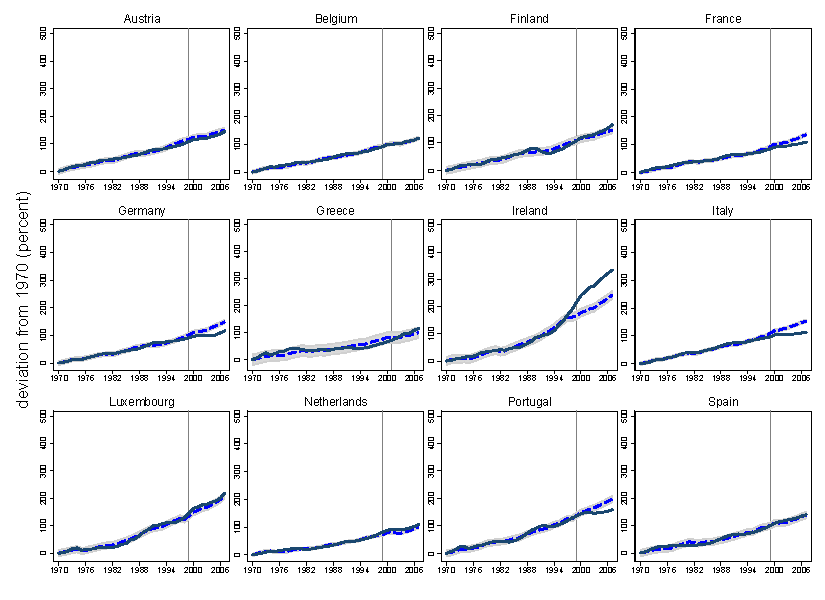
\includegraphics[width=\textwidth]{Output/Figures/images/SCM_normgdppc_Annual.pdf}
    \annote{In each graph, the dashed line represents the normalized real GDP per capita for the synthetic country and the continuous line represents the series for the actual country. The shaded area corresponds to two standard deviations of the difference between the treated country and the doppelganger before the euro accession. The vertical line represents the treatment period - 1999 for all countries except for Greece which is 2001. For each country, the analysis starts in 1970 and ends in 2007. }
    \label{F_normgdppc}
\end{figure}


\clearpage
\begin{landscape}
\subsection{RMSPE}
\begin{table}[htbp]
\scriptsize
\caption{\label{TA_RMSPE} Relative RMSPE of the Pre- and Post-Treatment Doppelganger gaps.}\centering\medskip
\begin{tabular}{cccccccccccccccc|c} \toprule
                      & \textit{\textbf{AUS}} & \textit{\textbf{CAN}} & \textit{\textbf{CHL}} & \textit{\textbf{DNK}} & \textit{\textbf{ISL}} & \textit{\textbf{ISR}}  & \textit{\textbf{KOR}} & \textit{\textbf{MEX}} & \textit{\textbf{NZL}} & \textit{\textbf{NOR}} & \textit{\textbf{SWE}} & \textit{\textbf{CHE}} & \textit{\textbf{GBR}} & \textit{\textbf{USA}} & \textit{\textbf{Treated}} & \textit{\textbf{P-Value ($\rho$)}} \\ \midrule
\textit{\textbf{AUT}} & 2.98 & 5.00 & 2.85 & 4.50 & 1.73 & 1.25 & 2.93 & 4.35 & 3.10 & 7.64 & 4.41 & 3.24 & 1.16 & 3.97 & 3.20  & 0.533  \\
\textit{\textbf{BEL}} & 2.86 & 4.57 & 2.85 & 5.97 & 3.01 & 1.79 & 2.93 & 4.35 & 3.28 & 5.66 & 4.41 & 3.24 & 1.51 & 5.19 & 3.40  & 0.467 \\
\textit{\textbf{FIN}} & 2.61 & 5.28 & 2.85 & 4.42 & 2.89 & 1.25 & 2.93 & 4.35 & 3.30 & 7.65 & 3.64 & 3.24 & 1.33 & 3.88 & 1.78  & 0.867 \\
\textit{\textbf{FRA}} & 2.99 & 2.49 & 2.85 & 4.34 & 1.61 & 1.25 & 2.93 & 4.35 & 3.14 & 7.37 & 2.47 & 3.24 & 1.54 & 4.04 & 4.97  & \textbf{0.133} \\
\textit{\textbf{DEU}} & 2.80 & 4.74 & 2.85 & 4.98 & 2.88 & 1.25 & 2.93 & 4.35 & 3.30 & 7.65 & 4.40 & 3.24 & 1.22 & 2.86 & 5.98  & \textbf{0.133} \\
\textit{\textbf{GRC}} & 2.81 & 3.83 & 2.59 & 4.83 & 3.49 & 2.38 & 2.74 & 5.15 & 3.63 & 5.93 & 4.66 & 3.04 & 1.33 & 5.21 & 0.48  & 1.000\\
\textit{\textbf{IRL}} & 2.81 & 5.34 & 1.04 & 4.37 & 2.00 & 8.16 & 2.93 & 4.35 & 2.81 & 8.77 & 4.40 & 3.24 & 1.82 & 5.19 & 15.51 & \textbf{0.067} \\
\textit{\textbf{ITA}} & 1.95 & 3.65 & 2.85 & 4.82 & 1.82 & 1.25 & 2.93 & 3.52 & 3.16 & 7.65 & 4.40 & 3.24 & 1.17 & 5.38 & 7.88  & \textbf{0.067} \\
\textit{\textbf{LUX}} & 2.70 & 5.69 & 2.85 & 5.90 & 1.97 & 1.25 & 2.93 & 4.35 & 2.71 & 7.35 & 4.40 & 3.24 & 2.43 & 3.88 & 3.69  & 0.467  \\
\textit{\textbf{NLD}} & 2.95 & 5.74 & 2.85 & 7.06 & 2.56 & 1.25 & 2.93 & 4.35 & 2.55 & 7.45 & 4.41 & 3.24 & 1.61 & 3.87 & 1.79  & 0.867  \\
\textit{\textbf{PRT}} & 3.02 & 5.23 & 2.85 & 4.70 & 3.01 & 1.27 & 2.93 & 3.66 & 2.88 & 7.50 & 4.40 & 3.24 & 1.85 & 3.86 & 6.26  & \textbf{0.133} \\
\textit{\textbf{ESP}} & 1.95 & 4.84 & 2.85 & 4.81 & 1.77 & 1.25 & 2.93 & 4.35 & 3.24 & 7.65 & 4.40 & 3.24 & 1.77 & 3.92 & 1.45  & 0.933 \\
\bottomrule
\end{tabular} 
\annote{The column \textit{Treated} displays the RMSPE ratio for each country, $\chi$ in equation \ref{EQ_test}. The column \textit{P-Value} tell us the chances of obtaining a ratio as high as the treated country if one were to pick a country at random from the sample including also the treated country (equivalent to $\rho$ in equation \ref{EQ_test2}). Given the small number of donor countries, we consider the results sizeable if there at most 2 countries with a higher RMSPE ratio.}
\end{table}

\end{landscape}

\clearpage

\subsection{In-Time Placebo Test}
\begin{figure}[h!]
    \centering
    \caption{In-Time Placebo Test - 1995 \label{F_1995}}
    \includegraphics[scale=1.2]{Maastricht_1995.eps}
    \annote{In each graph, the blue dashed line represents the normalized real GDP for the synthetic country and the black full line represents the series for the actual country. The shaded area corresponds to two standard deviations of the difference between the treated country and the doppelganger prior to the euro accession. The vertical line depicts the placebo treatment period - 1995 for all countries. For all countries the analysis starts in 1970 and ends in 2007. 
    %This date is particularly useful to analyze because it is the one used by \cite{Puzzello2018}. The reasons on why we do not use it are explained in the main text with the most compelling being that Austria and Finland are being analyzed in our work but they joined the EU in 1995. %The baseline specification has as predictors labor productivity growth, employment share, and GDP shares from PENN Tables 9.1 data. OECD restricted donor pool.
    }
\end{figure}
\clearpage 
\begin{figure}[h!]
    \centering
    \caption{In-Time Placebo Test - 1998 \label{F_1998}}
    \includegraphics[scale=1.2]{Maastricht_1998.eps}
    \annote{In each graph, the blue dashed line represents the normalized real GDP for the synthetic country and the black full line represents the series for the actual country. The shaded area corresponds to two standard deviations of the difference between the treated country and the doppelganger prior to the euro accession. The vertical line depicts the placebo treatment period - 1998 for all countries. For all countries the analysis starts in 1970 and ends in 2007.
    }
\end{figure}


\subsection{Changing Donor Pool \label{SS_donor_appendix}}
In each of the following set of graphs, the blue dashed line represents the normalized real GDP for the synthetic country and the black full line represents the series for the actual country. The vertical line depicts the treatment period. For all countries the analysis starts in 1970 and ends in 2007. We iteratively exclude different countries from the donor pool as argued in Section \ref{SS_donor}.

\begin{figure}[h!]
    \centering
    \label{F_AUS}
    \caption{SCM without Australia}
    \includegraphics[scale=0.7]{SCM_without_AUS.eps}
     \annote{In each graph, the blue dashed line represents the normalized real GDP for the synthetic country and the black full line represents the series for the actual country. The shaded area corresponds to two standard deviations of the difference between the treated country and the doppelganger prior to the euro accession. The vertical line depicts the placebo treatment period - 2001 for Greece and 1999 for all other countries. For all countries the analysis starts in 1970 and ends in 2007. Australia is excluded from the donor pool. }
\end{figure}

\begin{figure}[h!]
    \centering
    \label{F_AUS}
    \caption{SCM without Australia}
    \includegraphics[scale=0.7]{SCM_without_AUS.eps}
     \annote{In each graph, the blue dashed line represents the normalized real GDP for the synthetic country and the black full line represents the series for the actual country. The shaded area corresponds to two standard deviations of the difference between the treated country and the doppelganger prior to the euro accession. The vertical line depicts the placebo treatment period - 2001 for Greece and 1999 for all other countries. For all countries the analysis starts in 1970 and ends in 2007. Australia is excluded from the donor pool. }
\end{figure}

\begin{figure}[h!]
    \centering
    \label{F_ISR}
    \caption{SCM without Israel}
    \includegraphics[scale=0.7]{SCM_without_ISR.eps}
         \annote{In each graph, the blue dashed line represents the normalized real GDP for the synthetic country and the black full line represents the series for the actual country. The shaded area corresponds to two standard deviations of the difference between the treated country and the doppelganger prior to the euro accession. The vertical line depicts the placebo treatment period - 2001 for Greece and 1999 for all other countries. For all countries the analysis starts in 1970 and ends in 2007. Israel is excluded from the donor pool. }
\end{figure}

\begin{figure}[h!]
    \centering
    \label{F_MEX}
    \caption{SCM without Mexico}
    \includegraphics[scale=0.7]{SCM_without_MEX.eps}
         \annote{In each graph, the blue dashed line represents the normalized real GDP for the synthetic country and the black full line represents the series for the actual country. The shaded area corresponds to two standard deviations of the difference between the treated country and the doppelganger prior to the euro accession. The vertical line depicts the placebo treatment period - 2001 for Greece and 1999 for all other countries. For all countries the analysis starts in 1970 and ends in 2007. Mexico is excluded from the donor pool. }
\end{figure}

\begin{figure}[h!]
    \centering
    \label{F_NOR}
    \caption{SCM without Norway}
    \includegraphics[scale=0.7]{SCM_without_NOR.eps}
         \annote{In each graph, the blue dashed line represents the normalized real GDP for the synthetic country and the black full line represents the series for the actual country. The shaded area corresponds to two standard deviations of the difference between the treated country and the doppelganger prior to the euro accession. The vertical line depicts the placebo treatment period - 2001 for Greece and 1999 for all other countries. For all countries the analysis starts in 1970 and ends in 2007. Norway is excluded from the donor pool. }
\end{figure}

\begin{figure}[h!]
    \centering
    \label{F_CHE}
    \caption{SCM without Switzerland}
    \includegraphics[scale=0.7]{SCM_without_CHE.eps}
         \annote{In each graph, the blue dashed line represents the normalized real GDP for the synthetic country and the black full line represents the series for the actual country. The shaded area corresponds to two standard deviations of the difference between the treated country and the doppelganger prior to the euro accession. The vertical line depicts the placebo treatment period - 2001 for Greece and 1999 for all other countries. For all countries the analysis starts in 1970 and ends in 2007. Switzerland is excluded from the donor pool. }
\end{figure}

\begin{figure}[h!]
    \centering
    \label{F_USA}
    \caption{SCM without the United States}
    \includegraphics[scale=0.7]{SCM_without_USA.eps}
             \annote{In each graph, the blue dashed line represents the normalized real GDP for the synthetic country and the black full line represents the series for the actual country. The shaded area corresponds to two standard deviations of the difference between the treated country and the doppelganger prior to the euro accession. The vertical line depicts the placebo treatment period - 2001 for Greece and 1999 for all other countries. For all countries the analysis starts in 1970 and ends in 2007. The United States is excluded from the donor pool. }
\end{figure}

\section{\label{SS_Components} Components Analysis}

\begin{figure}[h!]
    \centering
    \caption{\label{F_Components_AUT} Components of Austria's GDP}
    \subfigure[Private Consumption]{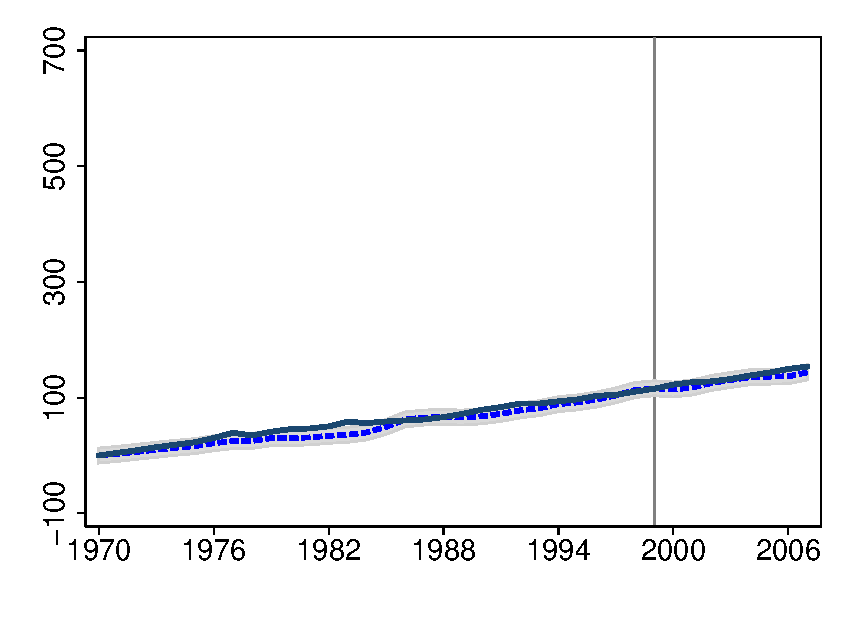
\includegraphics[width=8cm]{Composition/SCM_csh_c_1_Annual.eps}}
    \subfigure[Government Consumption]{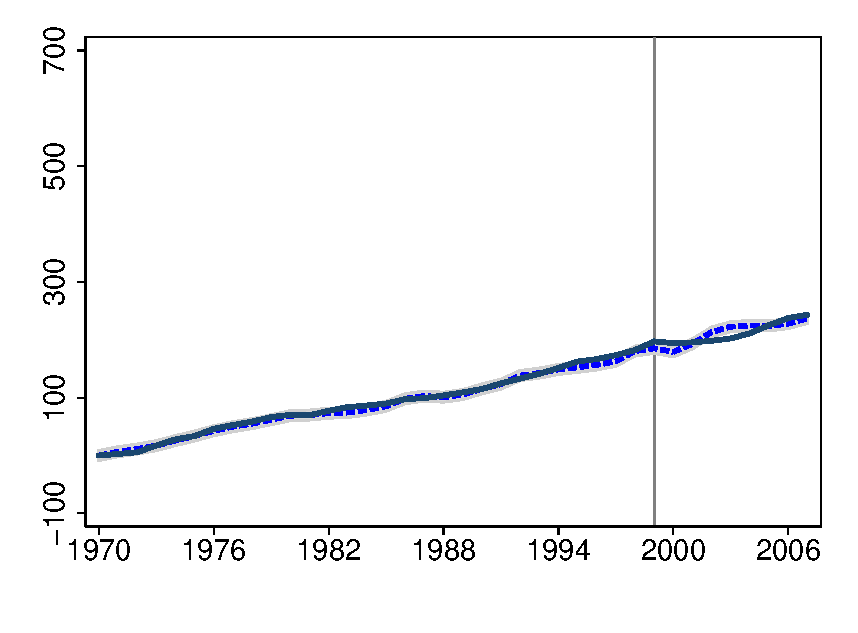
\includegraphics[width=8cm]{Composition/SCM_csh_g_1_Annual.eps}}
    \subfigure[Investment]{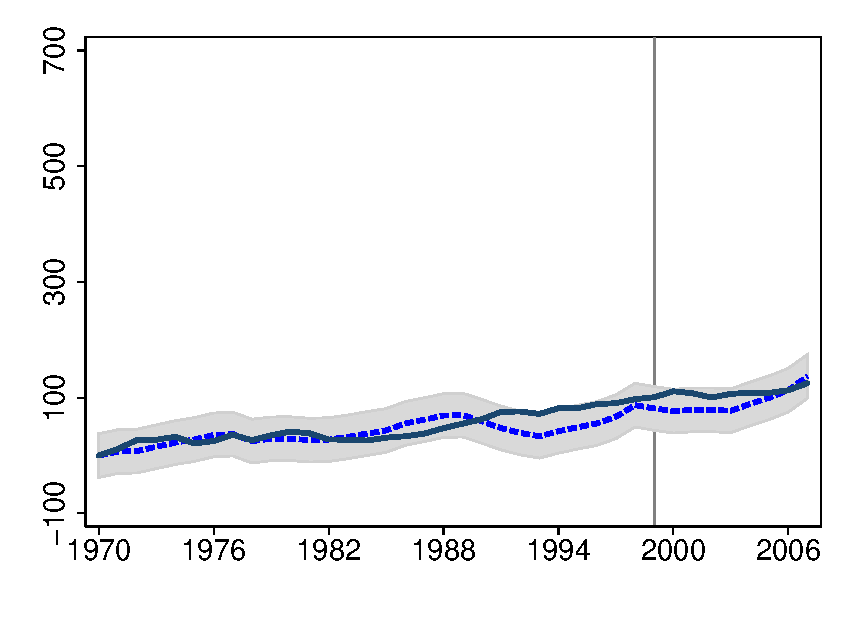
\includegraphics[width=8cm]{Composition/SCM_csh_i_1_Annual.eps}}
    \subfigure[Exports]{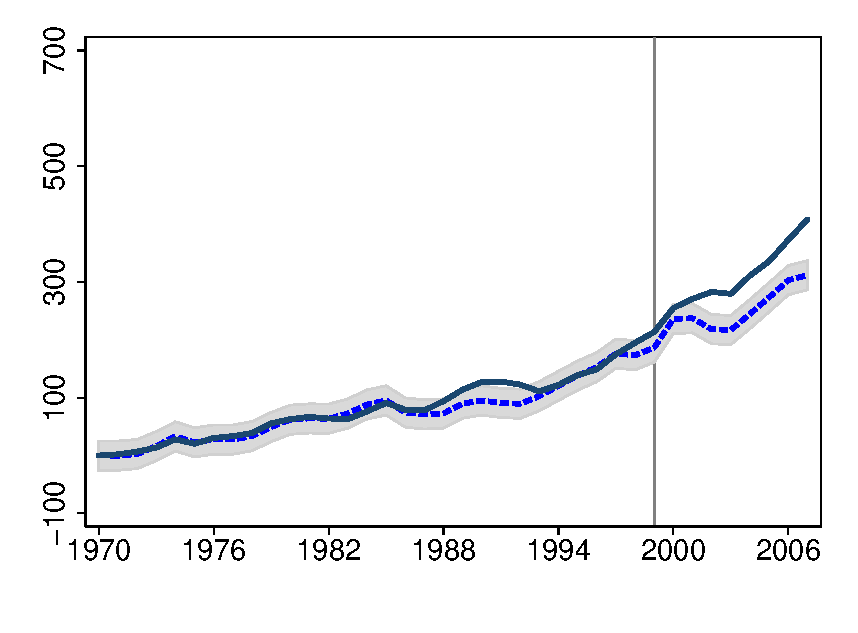
\includegraphics[width=8cm]{Composition/SCM_csh_x_1_Annual.eps}}
    \subfigure[Imports]{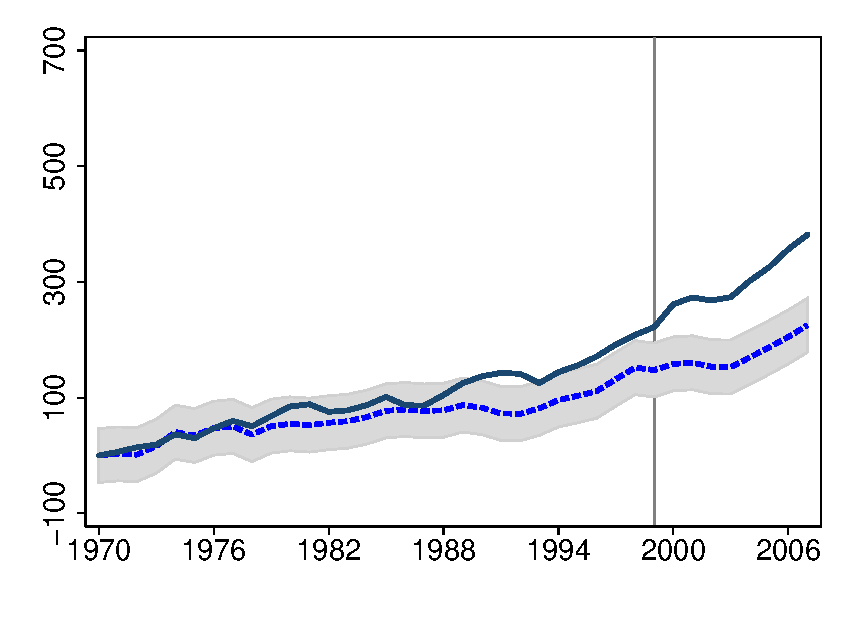
\includegraphics[width=8cm]{Composition/SCM_csh_m_1_Annual.eps}}
    \subfigure[Net Exports]{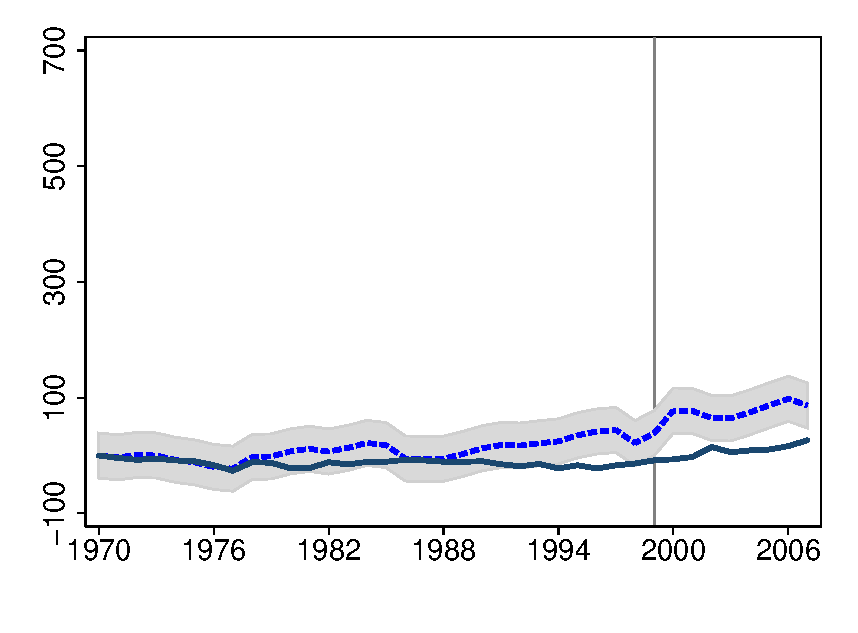
\includegraphics[width=8cm]{Composition/SCM_csh_nx_1_Annual.eps}}
    \annote{The plots depict, for each GDP component, the deviation in percent from the value of 1970. The blue dashed lines represents the synthetic Austria computed in section \ref{S_Doppelganger}. The full black lines stand for the actual Austrian series. The shaded area corresponds to two standard deviations of the difference between the treated country and the doppelganger prior to the euro accession.}
\end{figure}

\begin{figure}[h!]
    \centering
    \caption{\label{F_Components_BEL} Components of Belgium's GDP}
    \subfigure[Private Consumption]{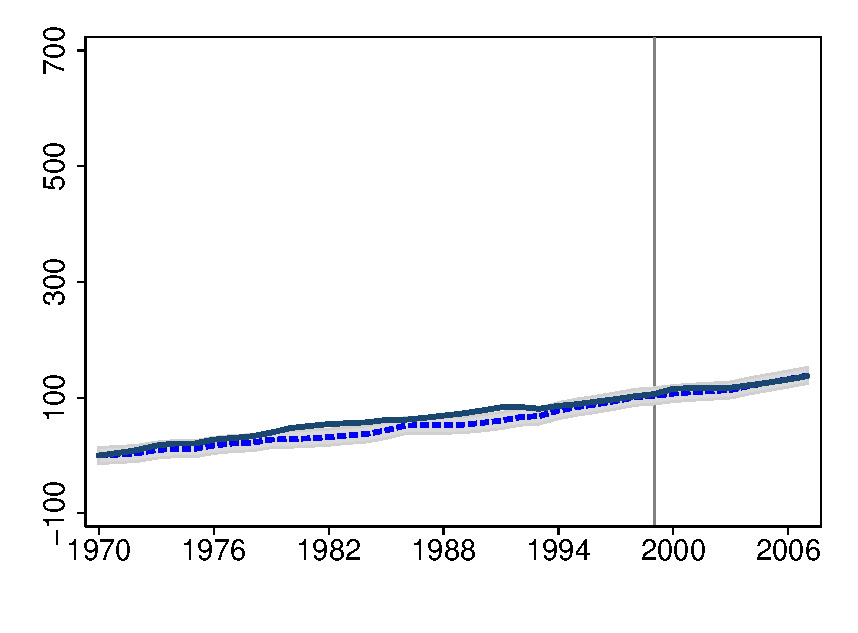
\includegraphics[width=8cm]{Composition/SCM_csh_c_3_Annual.eps}}
    \subfigure[Government Consumption]{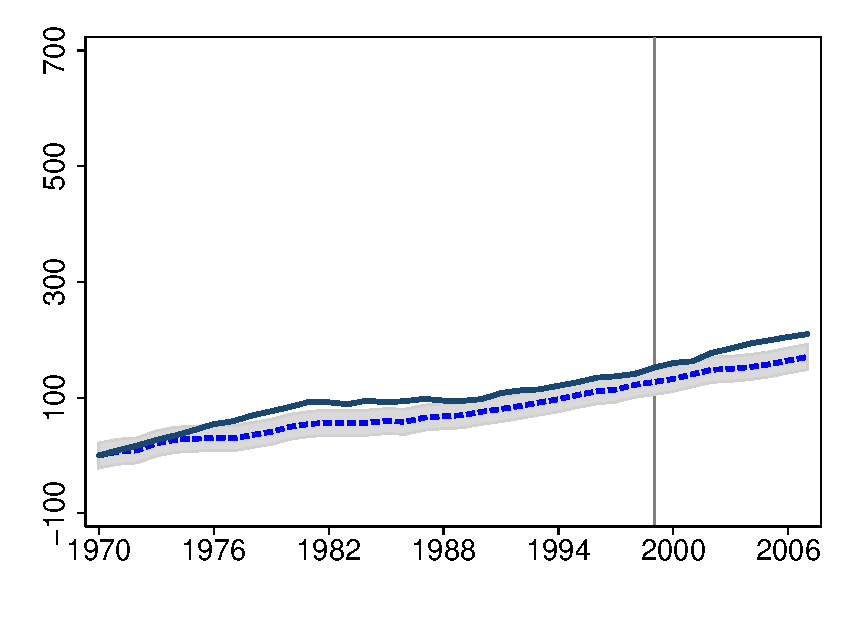
\includegraphics[width=8cm]{Composition/SCM_csh_g_3_Annual.eps}}
    \subfigure[Investment]{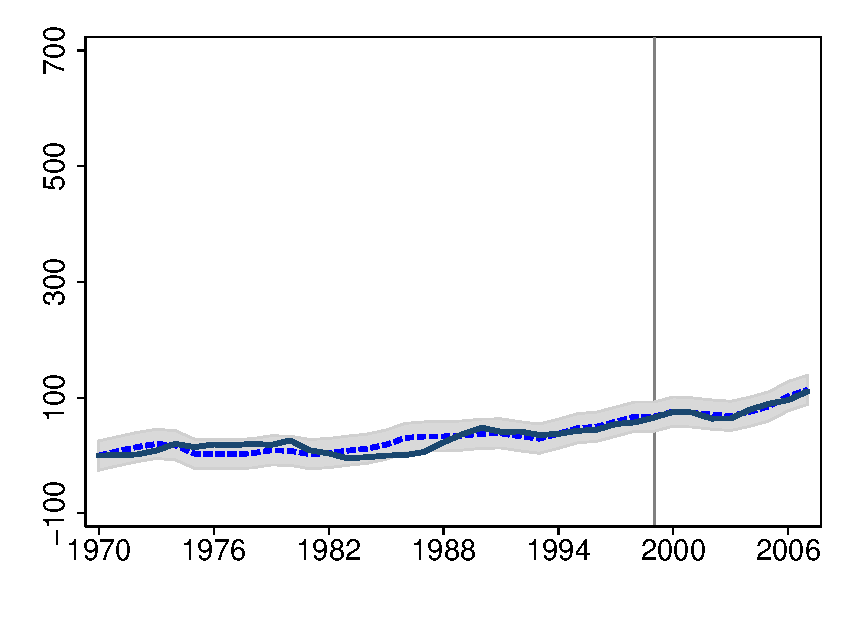
\includegraphics[width=8cm]{Composition/SCM_csh_i_3_Annual.eps}}
    \subfigure[Exports]{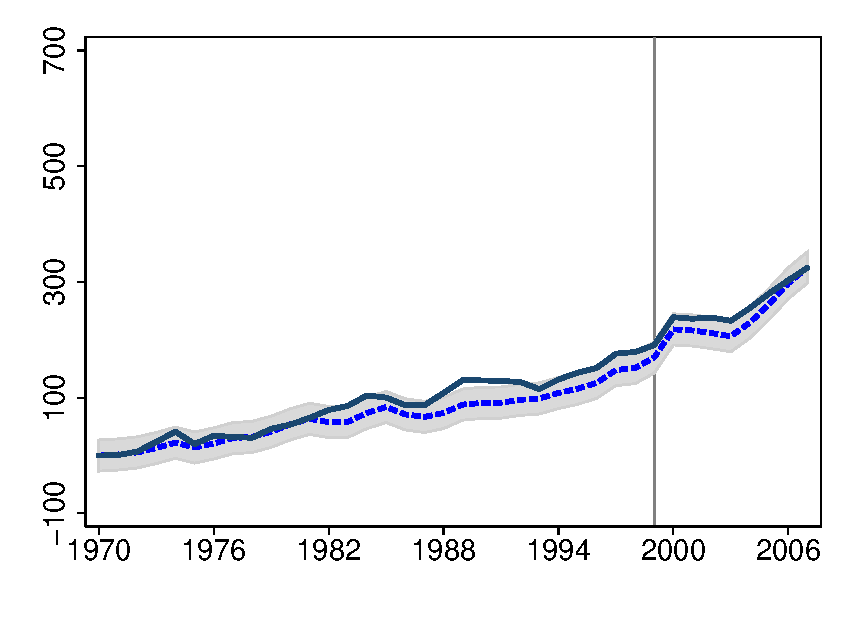
\includegraphics[width=8cm]{Composition/SCM_csh_x_3_Annual.eps}}
    \subfigure[Imports]{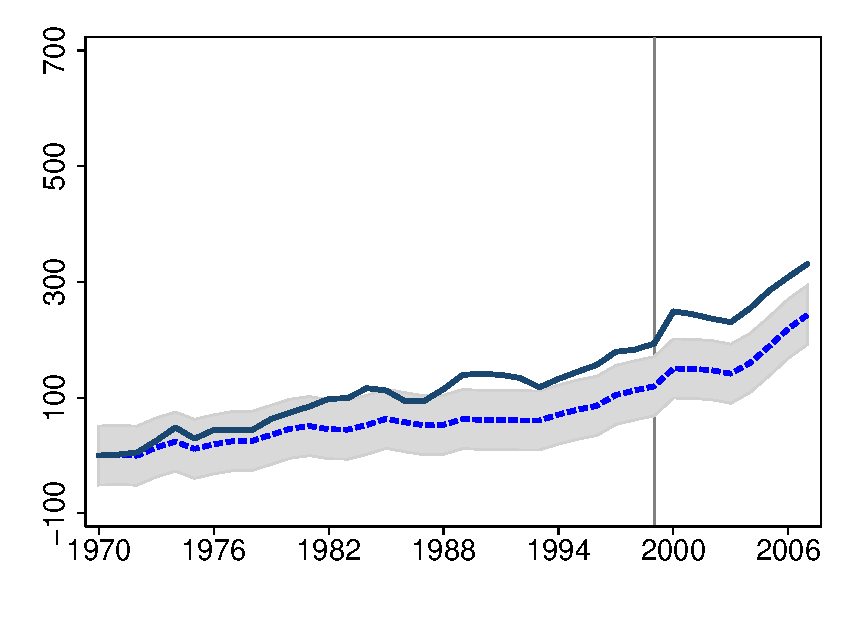
\includegraphics[width=8cm]{Composition/SCM_csh_m_3_Annual.eps}}
    \subfigure[Net Exports]{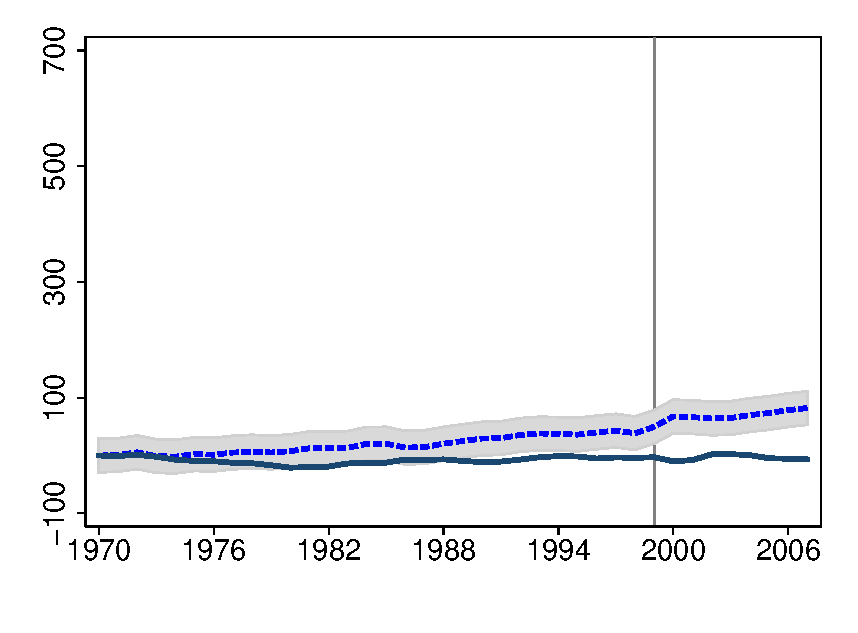
\includegraphics[width=8cm]{Composition/SCM_csh_nx_3_Annual.eps}}
    \annote{The plots depict, for each GDP component, the deviation in percent from the value of 1970. The blue dashed lines represents the synthetic Austria computed in section \ref{S_Doppelganger}. The full black lines stand for the actual Belgian series. The shaded area corresponds to two standard deviations of the difference between the treated country and the doppelganger prior to the euro accession. }
\end{figure}

\begin{figure}[h!]
    \centering
    \caption{\label{F_Components_FIN} Components of Finland's GDP}
    \subfigure[Private Consumption]{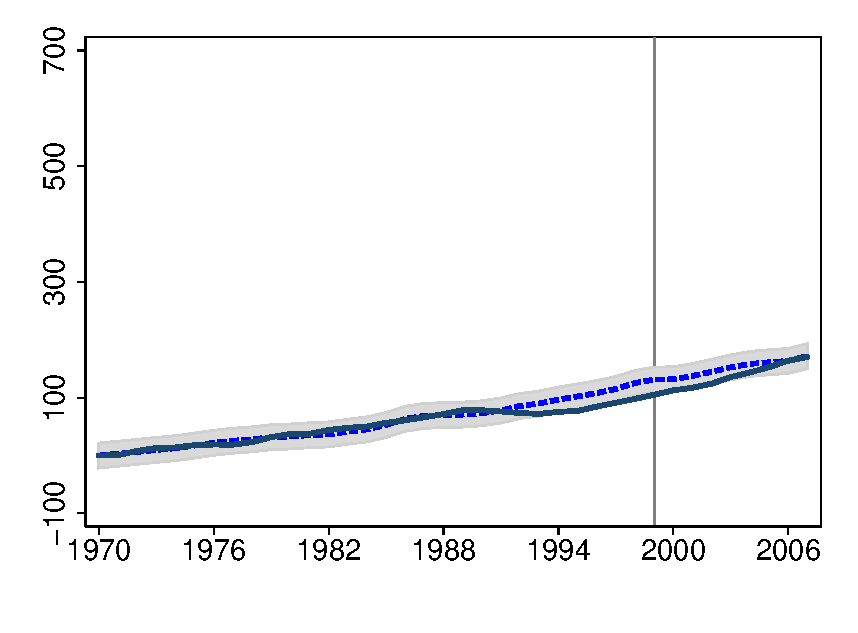
\includegraphics[width=8cm]{Composition/SCM_csh_c_7_Annual.eps}}
    \subfigure[Government Consumption]{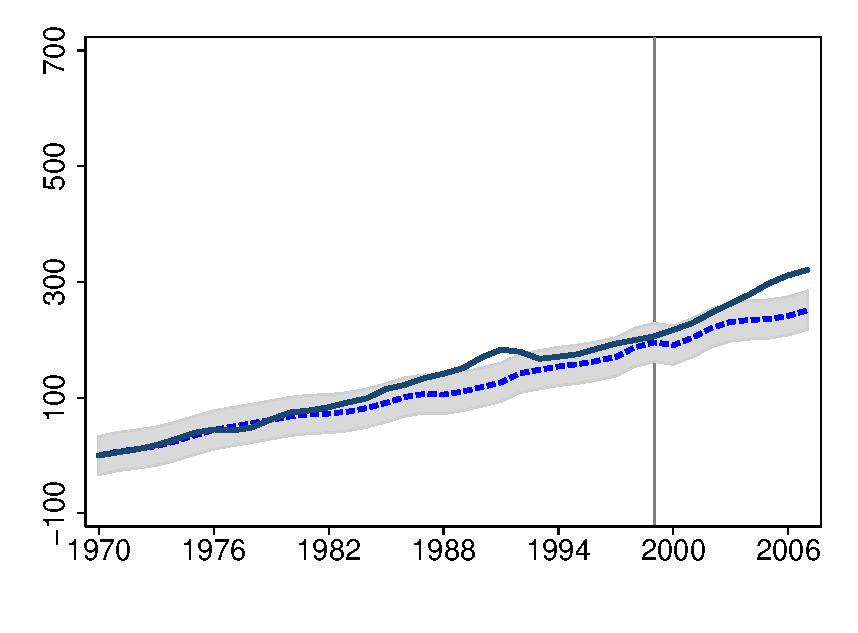
\includegraphics[width=8cm]{Composition/SCM_csh_g_7_Annual.eps}}
    \subfigure[Investment]{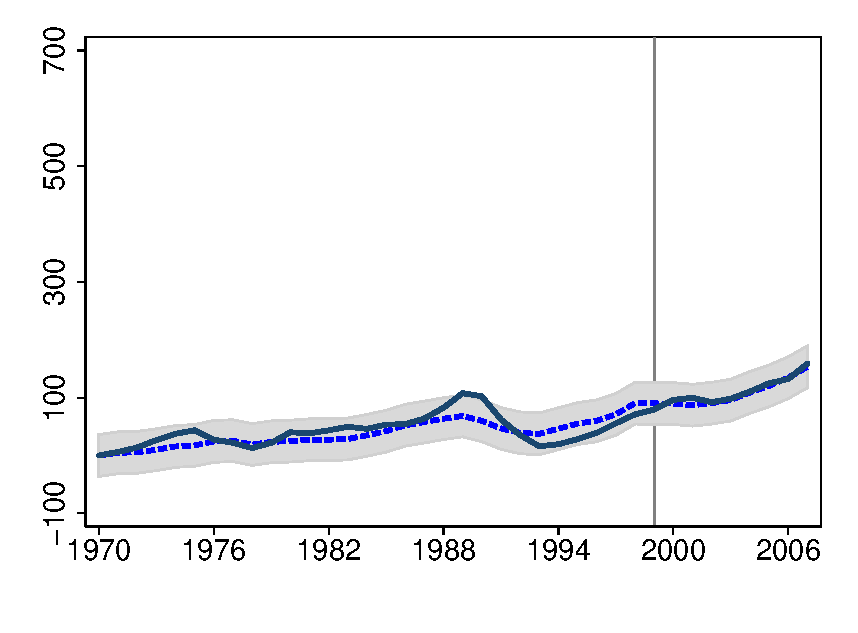
\includegraphics[width=8cm]{Composition/SCM_csh_i_7_Annual.eps}}
    \subfigure[Exports]{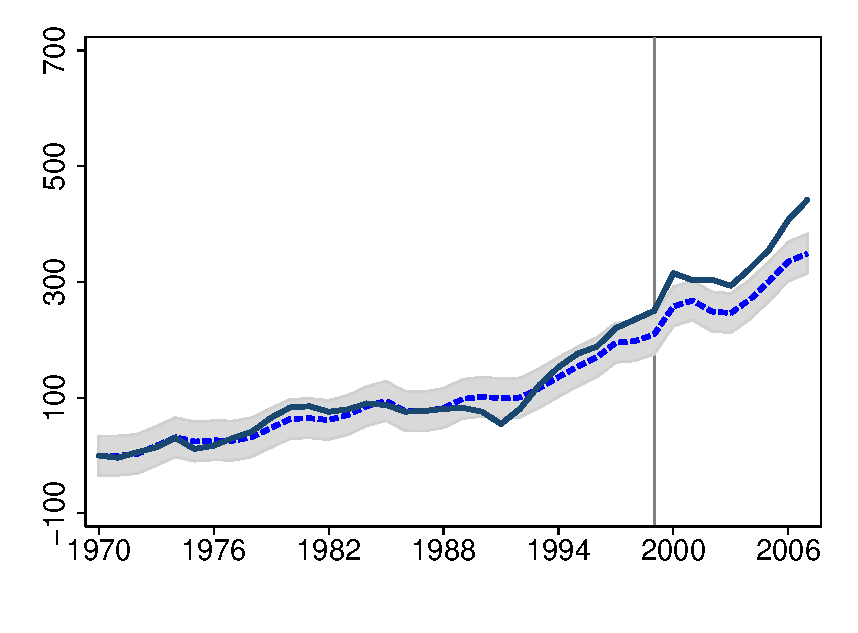
\includegraphics[width=8cm]{Composition/SCM_csh_x_7_Annual.eps}}
    \subfigure[Imports]{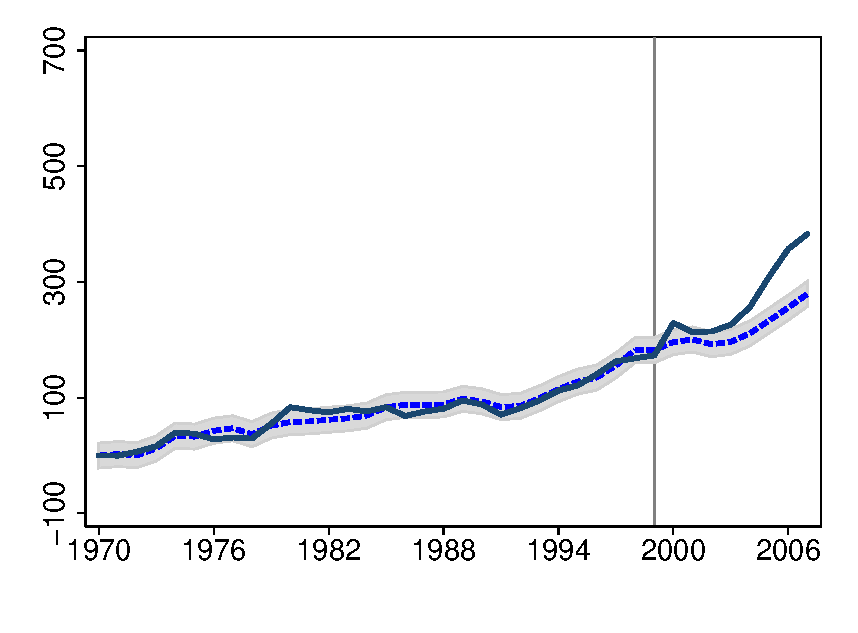
\includegraphics[width=8cm]{Composition/SCM_csh_m_7_Annual.eps}}
    \subfigure[Net Exports]{\includegraphics[width=8cm]{Composition/SCM_csh_nx_7_Annual.eps}}
    \annote{The plots depict, for each GDP component, the deviation in percent from the value of 1970. The blue dashed lines represents the synthetic Belgium computed in section \ref{S_Doppelganger}. The full black lines stand for the actual Finnish series. The shaded area corresponds to two standard deviations of the difference between the treated country and the doppelganger prior to the euro accession. }
\end{figure}

\begin{figure}[h!]
    \centering
    \caption{\label{F_Components_FRA} Components of France's GDP}
    \subfigure[Private Consumption]{\includegraphics[width=8cm]{Composition/SCM_csh_c_8_Annual.eps}}
    \subfigure[Government Consumption]{\includegraphics[width=8cm]{Composition/SCM_csh_g_8_Annual.eps}}
    \subfigure[Investment]{\includegraphics[width=8cm]{Composition/SCM_csh_i_8_Annual.eps}}
    \subfigure[Exports]{\includegraphics[width=8cm]{Composition/SCM_csh_x_8_Annual.eps}}
    \subfigure[Imports]{\includegraphics[width=8cm]{Composition/SCM_csh_m_8_Annual.eps}}
    \subfigure[Net Exports]{\includegraphics[width=8cm]{Composition/SCM_csh_nx_8_Annual.eps}}
    \annote{The plots depict, for each GDP component, the deviation in percent from the value of 1970. The blue dashed lines represents the synthetic France computed in section \ref{S_Doppelganger}. The full black lines stand for the actual French series. The shaded area corresponds to two standard deviations of the difference between the treated country and the doppelganger prior to the euro accession. }
\end{figure}

\begin{figure}[h!]
    \centering
    \caption{\label{F_Components_DEU} Components of Germany's GDP}
    \subfigure[Private Consumption]{\includegraphics[width=8cm]{Composition/SCM_csh_c_9_Annual.eps}}
    \subfigure[Government Consumption]{\includegraphics[width=8cm]{Composition/SCM_csh_g_9_Annual.eps}}
    \subfigure[Investment]{\includegraphics[width=8cm]{Composition/SCM_csh_i_9_Annual.eps}}
    \subfigure[Exports]{\includegraphics[width=8cm]{Composition/SCM_csh_x_9_Annual.eps}}
    \subfigure[Imports]{\includegraphics[width=8cm]{Composition/SCM_csh_m_9_Annual.eps}}
    \subfigure[Net Exports]{\includegraphics[width=8cm]{Composition/SCM_csh_nx_9_Annual.eps}}
    \annote{The plots depict, for each GDP component, the deviation in percent from the value of 1970. The blue dashed lines represents the synthetic Germany computed in section \ref{S_Doppelganger}. The full black lines stand for the actual German series. The shaded area corresponds to two standard deviations of the difference between the treated country and the doppelganger prior to the euro accession. }
\end{figure}

\begin{figure}[h!]
    \centering
    \caption{\label{F_Components_GRC} Components of Greece's GDP}
    \subfigure[Private Consumption]{\includegraphics[width=8cm]{Composition/SCM_csh_c_10_Annual.eps}}
    \subfigure[Government Consumption]{\includegraphics[width=8cm]{Composition/SCM_csh_g_10_Annual.eps}}
    \subfigure[Investment]{\includegraphics[width=8cm]{Composition/SCM_csh_i_10_Annual.eps}}
    \subfigure[Exports]{\includegraphics[width=8cm]{Composition/SCM_csh_x_10_Annual.eps}}
    \subfigure[Imports]{\includegraphics[width=8cm]{Composition/SCM_csh_m_10_Annual.eps}}
    \subfigure[Net Exports]{\includegraphics[width=8cm]{Composition/SCM_csh_nx_10_Annual.eps}}
    \annote{The plots depict, for each GDP component, the deviation in percent from the value of 1970. The blue dashed lines represents the synthetic Greece computed in section \ref{S_Doppelganger}. The full black lines stand for the actual Greek series. The shaded area corresponds to two standard deviations of the difference between the treated country and the doppelganger prior to the euro accession. }
\end{figure}

\begin{figure}[h!]
    \centering
    \caption{\label{F_Components_IRL} Components of Ireland's GDP}
    \subfigure[Private Consumption]{\includegraphics[width=8cm]{Composition/SCM_csh_c_12_Annual.eps}}
    \subfigure[Government Consumption]{\includegraphics[width=8cm]{Composition/SCM_csh_g_12_Annual.eps}}
    \subfigure[Investment]{\includegraphics[width=8cm]{Composition/SCM_csh_i_12_Annual.eps}}
    \subfigure[Exports]{\includegraphics[width=8cm]{Composition/SCM_csh_m_12_Annual.eps}}
    \subfigure[Imports]{\includegraphics[width=8cm]{Composition/SCM_csh_x_12_Annual.eps}}
    \subfigure[Net Exports]{\includegraphics[width=8cm]{Composition/SCM_csh_nx_12_Annual.eps}}
    \annote{The plots depict, for each GDP component, the deviation in percent from the value of 1970. The blue dashed lines represents the synthetic Ireland computed in section \ref{S_Doppelganger}. The full black lines stand for the actual Irish series. The shaded area corresponds to two standard deviations of the difference between the treated country and the doppelganger prior to the euro accession. }
\end{figure}

\begin{figure}[h!]
    \centering
    \caption{\label{F_Components_ITA} Components of Italy's GDP}
    \subfigure[Private Consumption]{\includegraphics[width=8cm]{Composition/SCM_csh_c_14_Annual.eps}}
    \subfigure[Government Consumption]{\includegraphics[width=8cm]{Composition/SCM_csh_g_14_Annual.eps}}
    \subfigure[Investment]{\includegraphics[width=8cm]{Composition/SCM_csh_i_14_Annual.eps}}
    \subfigure[Exports]{\includegraphics[width=8cm]{Composition/SCM_csh_m_14_Annual.eps}}
    \subfigure[Imports]{\includegraphics[width=8cm]{Composition/SCM_csh_x_14_Annual.eps}}
    \subfigure[Net Exports]{\includegraphics[width=8cm]{Composition/SCM_csh_nx_14_Annual.eps}}
    \annote{The plots depict, for each GDP component, the deviation in percent from the value of 1970. The blue dashed lines represents the synthetic Italy computed in section \ref{S_Doppelganger}. The full black lines stand for the actual Italian series. The shaded area corresponds to two standard deviations of the difference between the treated country and the doppelganger prior to the euro accession. }
\end{figure}

\begin{figure}[h!]
    \centering
    \caption{\label{F_Components_LUX} Components of Luxembourg's GDP}
    \subfigure[Private Consumption]{\includegraphics[width=8cm]{Composition/SCM_csh_c_16_Annual.eps}}
    \subfigure[Government Consumption]{\includegraphics[width=8cm]{Composition/SCM_csh_g_16_Annual.eps}}
    \subfigure[Investment]{\includegraphics[width=8cm]{Composition/SCM_csh_i_16_Annual.eps}}
    \subfigure[Exports]{\includegraphics[width=8cm]{Composition/SCM_csh_x_16_Annual.eps}}
    \subfigure[Imports]{\includegraphics[width=8cm]{Composition/SCM_csh_m_16_Annual.eps}}
    \subfigure[Net Exports]{\includegraphics[width=8cm]{Composition/SCM_csh_nx_16_Annual.eps}}
    \annote{The plots depict, for each GDP component, the deviation in percent from the value of 1970. The blue dashed lines represents the synthetic Luxembourg computed in section \ref{S_Doppelganger}. The full black lines stand for the actual Luxembourg's series. The shaded area corresponds to two standard deviations of the difference between the treated country and the doppelganger prior to the euro accession. }
\end{figure}

\begin{figure}[h!]
    \centering
    \caption{\label{F_Components_NLD} Components of The Netherlands's GDP}
    \subfigure[Private Consumption]{\includegraphics[width=8cm]{Composition/SCM_csh_c_18_Annual.eps}}
    \subfigure[Government Consumption]{\includegraphics[width=8cm]{Composition/SCM_csh_g_18_Annual.eps}}
    \subfigure[Investment]{\includegraphics[width=8cm]{Composition/SCM_csh_i_18_Annual.eps}}
    \subfigure[Exports]{\includegraphics[width=8cm]{Composition/SCM_csh_x_18_Annual.eps}}
    \subfigure[Imports]{\includegraphics[width=8cm]{Composition/SCM_csh_m_18_Annual.eps}}
    \subfigure[Net Exports]{\includegraphics[width=8cm]{Composition/SCM_csh_nx_18_Annual.eps}}
    \annote{The plots depict, for each GDP component, the deviation in percent from the value of 1970. The blue dashed lines represents the synthetic Netherlands computed in section \ref{S_Doppelganger}. The full black lines stand for the actual Dutch series. The shaded area corresponds to two standard deviations of the difference between the treated country and the doppelganger prior to the euro accession.}
\end{figure}

\begin{figure}[h!]
    \centering
    \caption{\label{F_Components_PRT} Components of Portugal's GDP}
    \subfigure[Private Consumption]{\includegraphics[width=8cm]{Composition/SCM_csh_c_21_Annual.eps}}
    \subfigure[Government Consumption]{\includegraphics[width=8cm]{Composition/SCM_csh_g_21_Annual.eps}}
    \subfigure[Investment]{\includegraphics[width=8cm]{Composition/SCM_csh_i_21_Annual.eps}}
    \subfigure[Exports]{\includegraphics[width=8cm]{Composition/SCM_csh_x_21_Annual.eps}}
    \subfigure[Imports]{\includegraphics[width=8cm]{Composition/SCM_csh_m_21_Annual.eps}}
    \subfigure[Net Exports]{\includegraphics[width=8cm]{Composition/SCM_csh_nx_21_Annual.eps}}
    \annote{The plots depict, for each GDP component, the deviation in percent from the value of 1970. The blue dashed lines represents the synthetic Portugal computed in section \ref{S_Doppelganger}. The full black lines stand for the actual Portuguese series.  The shaded area corresponds to two standard deviations of the difference between the treated country and the doppelganger prior to the euro accession.}
\end{figure}

\begin{figure}[h!]
    \centering
    \caption{\label{F_Components_ESP} Components of Spain's GDP}
    \subfigure[Private Consumption]{\includegraphics[width=8cm]{Composition/SCM_csh_c_22_Annual.eps}}
    \subfigure[Government Consumption]{\includegraphics[width=8cm]{Composition/SCM_csh_g_22_Annual.eps}}
    \subfigure[Investment]{\includegraphics[width=8cm]{Composition/SCM_csh_i_22_Annual.eps}}
    \subfigure[Exports]{\includegraphics[width=8cm]{Composition/SCM_csh_x_22_Annual.eps}}
    \subfigure[Imports]{\includegraphics[width=8cm]{Composition/SCM_csh_m_22_Annual.eps}}
    \subfigure[Net Exports]{\includegraphics[width=8cm]{Composition/SCM_csh_nx_22_Annual.eps}}
    \annote{The plots depict, for each GDP component, the deviation in percent from the value of 1970. The blue dashed lines represents the synthetic Spain computed in section \ref{S_Doppelganger}. The full black lines stand for the actual Spanish series. The shaded area corresponds to two standard deviations of the difference between the treated country and the doppelganger prior to the euro accession.}
\end{figure}


\begin{landscape}
\begin{table}[htbp]
\scriptsize
\caption{\label{TA_weights_placebo}  Composition of the Doppelgangers: Country Weights (in \%)}\centering\medskip
\begin{tabular}{lcccccccccccc} \toprule
\textit{Donor countries} & Austria  & Belgium  & Finland  & France  & Germany  & Greece  & Ireland  & Italy  & Luxembourg  & Netherlands  & Portugal  & Spain  \\  \midrule
Australia &      $<0.1$ &       $<0.1$ &     $<0.1$ &       27.2 &       $<0.1$ &       $<0.1$ &       $<0.1$ &       13.4 &       $<0.1$ &       $<0.1$ &       $<0.1$ &       $<0.1$ \\  
Canada &       $<0.1$ &       $<0.1$ &      67.7 &     37.4 &      23.0 &       12.8 &       $<0.1$ &      27.4 &       $<0.1$ &       $<0.1$ &       $<0.1$ &       $<0.1$ \\  
Chile &       $<0.1$ &       $<0.1$ &       $<0.1$ &       0.1 &       $<0.1$ &      1.7 &      22.0 &       $<0.1$ &       5.2 &       $<0.1$ &       $<0.1$ &       $<0.1$ \\  
Iceland &       $<0.1$ &       $<0.1$ &      9.6 &       $<0.1$ &       $<0.1$ &       $<0.1$ &       $<0.1$ &       $<0.1$ &       $<0.1$ &       $<0.1$ &       $<0.1$ &       $<0.1$ \\  
Israel &     $<0.1$ &      $<0.1$ &       $<0.1$ &       $<0.1$ &       $<0.1$ &       $<0.1$ &      50.1 &       $<0.1$ &      56.0 &      12.0 &      $<0.1$ &       $<0.1$ \\  
Korea &       $<0.1$ &       $<0.1$ &       $<0.1$ &       $<0.1$ &       $<0.1$ &       $<0.1$ &       $<0.1$ &       $<0.1$ &       $<0.1$ &       $<0.1$ &       4.4 &       $<0.1$ \\  
Mexico &       23.2 &       $<0.1$ &       $<0.1$ &       $<0.1$ &       $<0.1$ &       19.6 &       $<0.1$ &      11.9 &       $<0.1$ &       $<0.1$ &      42.4 &      22.2 \\  
New Zealand &      7.5 &       $<0.1$ &       $<0.1$ &      19.8 &      $<0.1$ &    65.9 &       $<0.1$ &       39.7 &       $<0.1$ &       $<0.1$ &       $<0.1$ &       8.2 \\  
Norway &      25.3 &       41.9 &       $<0.1$ &      $<0.1$ &       $<0.1$ &       $<0.1$ &      27.9 &       $<0.1$ &       $<0.1$ &      22.6 &       $<0.1$ &       $<0.1$ \\  
Switzerland &      44.0 &      58.1 &      22.7 &       $<0.1$ &      43.1 &      $<0.1$ &       $<0.1$ &      $<0.1$ &      44.0 &      65.4 &     31.4 &      19.7 \\  
United States &       $<0.1$ &       $<0.1$ &       $<0.1$ &       15.5 &      33.9 &     $<0.1$ &       $<0.1$ &      7.6 &       $<0.1$ &       $<0.1$ &      21.8 &      49.9 \\
\bottomrule
\end{tabular}
\annote{This table summarizes the weights in percent attributed to each donor country to construct the synthetic treated units. Relative to the baseline analysis, the donor pool now excludes Denmark, Sweden and the United Kingdom.}
\end{table}


\end{landscape}


\subsection{What Explains the Doppelganger Gap?}

\begin{table}[htbp!]
\scriptsize
\caption{\label{T_Decomposition}What Explains the Cumulative Doppelganger Gap?} \centering
\begin{tabular}{l|cccc|cc} 
\toprule
& \textbf{Private}   & \textbf{Government}   & \multirow{2}{*}{\textbf{Investment}}  & \textbf{Net}  & \multicolumn{2}{c}{\multirow{2}{*}{\textbf{Doppelganger Gap}}} \\ 

& \textbf{Consumption}  & \textbf{Consumption}  &  &  \textbf{Exports}  &    & \\

& (\%)   & (\%)   &  (\%)    &  (\%)  & (\%)   & \texteuro \ per capita\\ 
\midrule

\textbf{Austria} &      0.80 &      2.20 &     -1.24 &     -3.98 &     -2.22 &   -682.34 \\
[1em]
\textbf{Belgium} &      0.35 &      6.87 &     -1.36 &     -8.24 &     -2.39 &   -678.66 \\  
[1em]
\textbf{Finland} &      7.10 &      0.50 &      1.52 &     -4.60 &      4.52 &   1,268.80 \\
[1em]
\textbf{France} &     -4.50 &      0.65 &     -2.58 &     -3.20 &     -9.62 &  -2,843.31 \\
[1em]
\textbf{Germany} &    -10.24 &      1.53 &     -6.30 &      0.98 &    -14.02 &  -4,863.67 \\
[1em]
\textbf{Greece} &      3.41 &      3.70 &      3.78 &    -11.62 &     -0.74 &   -153.15 \\
[1em]
\textbf{Ireland} &     15.76 &      6.65 &     17.35 &      0.23 &     40.00 &  10,960.80 \\  
[1em]
\textbf{Italy} &    -15.40 &     -2.53 &     -4.80 &      1.38 &    -21.35 &  -7,350.99 \\
[1em]
\textbf{Luxembourg} &    -17.05 &      4.02 &     -3.06 &     30.07 &     13.97 &   5,157.19 \\  
[1em]
\textbf{Netherlands} &     -4.28 &      6.05 &     -0.27 &     -0.98 &      0.52 &    168.33 \\  
[1em]
\textbf{Portugal} &     -9.21 &     -0.09 &     -1.75 &     -5.67 &    -16.72 &  -3,706.06 \\
[1em]
\textbf{Spain}  &     -3.35 &      2.21 &     12.46 &     -4.46 &      6.85 &   1,538.55 \\ 

\bottomrule
\end{tabular}
\annote{This table summarizes the cumulative doppelganger gaps for each euro member country and presents the channels driving the impact of the accession by decomposing GDP into its components. The doppelganger gap represents the percentage GDP gain or loss in 2007 from adopting the common currency, i.e. for country \textit{c} we define \textit{percent doppelganger gap}$_{2007,c}= (GDP_{2007,c} - GDP_{2007,c}^{dop})/GDP_{2007,c}^{dop}$. Then, the table shows the contribution of each GDP component for the GDP gain or loss. Values are constructed in a way to sum up to the doppelganger gap. The decomposition of net exports into exports and imports is presented in Table \ref{T_Decomposition_NX}.}
\end{table}

\begin{table}[h!]
\scriptsize
\caption{\label{T_Decomposition_NX} Net Exports Decomposition} \centering
\begin{tabular}{l|c|cc} \toprule

        & \textbf{Net Exports}  & \textbf{Exports}  & \textbf{Imports}  \\  \midrule
\textbf{Austria} &     -3.98 &      5.35 &      9.34 \\  
[1em]
\textbf{Belgium} &     -8.24 &     22.62 &     30.86 \\   
[1em]
\textbf{Finland} &     -4.60 &      1.63 &      6.23 \\ 
[1em]
\textbf{France} &     -3.20 &    -12.36 &     -9.17 \\
[1em]
\textbf{Germany} &      0.98 &     -5.71 &     -6.69 \\  
[1em]
\textbf{Greece} &    -11.62 &     -5.60 &      6.02 \\
[1em]
\textbf{Ireland} &      0.23 &     69.65 &     69.42 \\
[1em]
\textbf{Italy} &      1.38 &     -2.75 &     -4.13 \\  
[1em]
\textbf{Luxembourg} &     30.07 &    153.19 &    123.12 \\ 
[1em]
\textbf{Netherlands} &     -0.98 &     15.38 &     16.35 \\   
[1em]
\textbf{Portugal} &     -5.67 &     -3.13 &      2.54 \\  
[1em]
\textbf{Spain} &     -4.46 &      1.64 &      6.10 \\
\bottomrule
\end{tabular}
\annote{This table presents the summary of the net exports decomposition into exports and imports for each treated country. It tells how much the net exports contributed to the doppelganger output gap in percent. }
%For example, the Austrian GDP is 4.96\% smaller than of its doppelganger due to net exports. Even though exports contributed to an increase of 5.56\% of GDP, imports contributed to a decrease of about 10.52\% of GDP.

\end{table}

\end{appendices}


\end{document}
